\documentclass[12pt,a4paper]{report}

\usepackage[dutch]{babel}

\usepackage{geometry}
\geometry{a4paper}

\usepackage{graphicx}
\usepackage{url}

\usepackage{longtable}
\usepackage{rotating}
\usepackage{array}
\usepackage{booktabs}
\usepackage{pdflscape}

\usepackage{hyperref}
\hypersetup{
    colorlinks,
    citecolor=black,
    filecolor=black,
    linkcolor=black,
    urlcolor=black
}

\begin{document}

%  Titelblad

\begin{titlepage}

\fontsize{12pt}{14pt}\selectfont

\begin{center}

\vspace{1cm}

\fontsize{14pt}{17pt}\selectfont
% De Faculteit:
\textsc{P\&O Computerwetenschappen - Verslag \\Team Platinum}
\fontsize{12pt}{14pt}\selectfont
\vspace{0.3cm}

\vspace{1.2cm}

%Het academiejaar: aanpassen!
Academiejaar 2011--2012

\vspace{2.8cm}

\fontsize{17.28pt}{21pt}\selectfont

% De titel van de thesis:
{\textsc{Pac-Man in de echte wereld,\\ met behulp van Lego Mindstorms}}

\fontseries{m}
\fontsize{12pt}{14pt}\selectfont

\vspace{2cm}


\includegraphics[height=10cm]{resources/Logo-Kul}

\end{center}
\end{titlepage}

\thispagestyle{empty}

\tableofcontents

\begin{abstract}
Tijdens de uitwerking van dit jaar-overschrijdend groepswerk, bouwen wij een autonome robot met behulp van Lego Mindstorms. Voor de programmatie wordt beroep gedaan op Lejos, een Open Bron project dat een minimale JAVA virtuele machine heeft gemaakt die de plaats kan innemen van de standaard programmatie omgeving van Lego.

Naast de doelstelling om kennis te maken met het ontwikkelen van een autonome robot, willen we in dit project ook ervaring opdoen i.v.m.\ het werken in teamverband aan een middelgroot softwareproject. Hierbij zijn organisatie van werk, planning, analyse, architectuur,... belangrijke begrippen.

In het tweede semester wordt hier nog eens de nood tot samenwerking met de andere teams aan toegevoegd. Het traject van de autonome robot blijft behouden, maar de verschillende robots zullen nu moeten samenwerken om een gemeenschappelijk doel te bereiken. Om deze samenwerking in goede banen te leiden werd een scheidsrechtercommissie in het leven geroepen om beslissingen te nemen die voor alle teams van belang zijn. Het doel van dit semester is het insluiten van een Pac-Manrobot bestuurd door het didactisch team met behulp van vier autonome \emph{ghosts}.

In het eerste semester werkten we reeds in een parallel traject aan een simulatieomgeving. Aan de hand van deze omgeving waren we in staat om met meerdere teamleden in parallel software voor de robot te ontwikkelen en te testen zonder nood aan een effectieve fysieke robot. Nu is het ontwikkelen van deze simulator deel geworden van de opdracht en dienen we dus de nodige aanpassingen te doen om het Pac-Manspel in de computer te simuleren. Het gebruik van een simulator is evident, aangezien we niet kunnen verwachten alle fysieke testen uit te voeren met de 4 teams tegelijk.
\end{abstract}

\chapter{Inleiding}

Het project wordt zoals in het eerste semester begeleid door het gebruik van tussentijdse demo's. Het doel is om zo optimaal mogelijk samen te werken met vier teams om de Pac-Man in te sluiten, hoewel we te allen tijden autonoom beslissingen nemen.

Het doel van de eerste demo is een vereenvoudigde vorm van het einddoel waarbij we een stilstaande Pac-Man zoeken binnen het doolhof. De simulator dient  reeds beschikbaar te zijn en moet drie virtuele robots de fysieke laten bijstaan. Voor de tweede demo mag de commissie beslissen welke doelstellingen passen in het verdere proces richting het einddoel.

Tijdens het eerste semester zijn we er in geslaagd om zeer herbruikbare code te produceren: de architecturale concepten, zoals \emph{Robot}, \emph{Navigator} en Model, zijn duidelijk binnen het team en de verdere uitwerking van deze concepten in het tweede semester werd ervaren als een natuurlijke evolutie. Aangezien we te maken hebben met een grote diversiteit aan kleine taken, gebeurt het grootste deel van de taakverdeling week op week.

Het verslag is anders opgebouwd ten opzichte van het vorige semester: er werd gekozen voor een onderverdeling in subsecties per demo binnen een context van hoofdstukken. De opbouw van deze hoofdstukken is erg gelijkend hoewel natuurlijk de inhoud veranderd is t.o.v.\ het eerste semester. Nieuw zijn de stukken over de strategie i.v.m.\ de opgegeven spelomgeving, over de samenwerking en over de finale analyse van het jaarproject.

\chapter{Probleemstelling}

De doelstellingen van de demo's worden hier achtereenvolgens beschreven. Zij volgen stapsgewijs een ontwerpproces dat tracht een autonome robot op te leveren die, samen met drie andere \emph{ghosts}, probeert de Pac-Man in te sluiten.

\section{Demo 1}

Het probleem dat we eerst aanpakken is het zo effici\"ent mogelijk in kaart brengen van een onbekende omgeving met behulp van de vier \emph{ghosts}. Belangrijk hierbij is natuurlijk dat de gedetecteerde wereld overeenkomt met de realiteit. Tijdens de demo gebruiken we een zgn. hybride simulator: onze eigen robot bestaat in de fysieke wereld, de andere drie zijn virtueel en worden vertegenwoordigd door drie virtuele \emph{ghosts} die in de simulator \emph{leven}.

De \emph{ghosts} hebben geen enkele informatie over het doolhof waarin ze zich bevinden, ze kennen wel hun eigen globale positie, maar dan weer niet hun ori\"entatie. Verder staat de Pac-Man stil in het parcours en dient hij enkel gevonden te worden. We dienen ook aan te tonen dat het door de commissie afgesproken communicatieprotocol ge\"implementeerd is.

Elk team wordt tijdens de demo afzonderlijk beoordeeld.
 
\section{Demo 2}
 
De doelstellingen voor demo 2 werden vastgelegd met de resultaten van de eerste demo in het achterhoofd. Deze waren voor sommige teams niet zo goed. Om de kern van de opdracht niet op de lange baan te schuiven wordt in demo 2 toch getracht een stap in de goede richting te nemen. Om de doelstellingen voor demo 2 haalbaar te houden, werd beslist om de Pac-Man nog steeds stil te laten staan. De tweede demo draait daarom volledig rond het samenwerken met de andere teams. Dit is duidelijk een van de essenti\"ele aspecten voor de uiteindelijke demo dat niet uit het oog mag verloren worden.

We volgen de raad op om op voorhand samen te zitten met de andere drie groepen. Het behalen van de doelstellingen is een inspanning van de vier teams samen. Om onverwachte resultaten te voorkomen is samen testen dan ook een noodzaak.

Het doel van deze demo ligt dus in het samen verkennen van het doolhof en het samen insluiten van een stilstaande Pac-Man. We doen dit zowel met de virtuele versie van de simulator als met de gedistribueerde. Initieel krijgt ook elk team de kans om eerst nogmaals zijn hybride simulator te tonen en de vooruitgang ten opzichte van de eerste demo aan te duiden.

\section{Demo 3}

\subsection{Verkenning}

De robots rijden in een onbekend doolhof. Alle info die verzameld wordt door de vier ghosts draagt bij tot het cre\"eren van een individuele map die mogelijk inconsistenties bevat. Alle juiste info over het doolhof zal direct bijdragen tot het hoofddoel, namelijk het vangen van de Pac-Man. Elke robot communiceert zijn gevonden informatie en probeert zo veel mogelijk informatie te verzamelen over de voor hem onbekende wereld. Elke fout van \'e\'en van de robots kan reeds fataal zijn voor het kunnen opbouwen van een beeld van de omgeving. We proberen dus een zo robuust mogelijke robot te maken die zo effici\"ent mogelijk zijn eigen info verzamelt en met de nodige voorzichtigheid andere informatie hierin verwerkt.

\subsection{Pac-Man}

Het Pac-Man spel zelf kunnen we winnen door alle vluchtwegen van de Pac-Man af te sluiten. Dit houdt in dat alle omliggende sectoren door een \emph{ghost} bezet of door een muur afgeschermd worden. Men wint enkel als alle robots die meewerken aan de insluiting ook effectief aangeven dat ze gewonnen hebben via hun grafische interface. De probleemstelling vereist dus een afdoende samenwerking, waarbij een consensus moet bereikt worden over de verzamelde informatie en de te volgen strategie.

\chapter{Scheidsrechtercommissie}

Deze commissie staat in voor het nemen van beslissingen die betrekking hebben op afspraken tussen de verschillende teams en het didactische team. Hierbij kunnen we deze beslissingen groeperen in:

\begin{itemize}
	\item De verdere regels waarmee de spelomgeving beperkt wordt.
	\item Afspraken die noodzakelijk zijn voor de samenwerking van de teams.
\end{itemize}

\section{Spelregels}

\subsection{Spelwereld}

De spelwereld bestaat uit aangepaste panelen uit het eerste semester. Er is een raster van witte lijnen ge\"introduceerd waar muren kunnen staan. Dit komt neer op een mogelijke herschaling van de panelen met een factor vier. Deze nieuwe minimumeenheid aan oppervlakte noemen we sectoren. Deze sectoren zijn belangrijk voor de plaatsbepaling. Het doolhof is volledig ommuurd en de absolute afmetingen worden op voorhand opgegeven.

\subsection{Pac-Man}

De Pac-Man wordt zichtbaar gemaakt door een infrarood-beacon dat kan opgemerkt worden met behulp van de voorziene IR-sensor. Het didactisch team kiest waar deze vertrekt en bestuurt hem tijdens de demo's. Hij mag enkel bewegen op sectoren waar zich geen \emph{ghosts} bevinden.

De beweging van Pac-Man is beperkt tot het rechtdoor oversteken van de witte lijnen die de sectoren scheiden.

Insluiting van Pac-Man is gedefinieerd als het niet meer kunnen bewegen van de Pac-Man of het ingesloten zijn in een doodlopend pad.

\subsection{Ghosts}

De ghosts vertrekken op de vier hoekpunten van het doolhof, zodat de verkenning van het doolhof zo snel mogelijk van start kan gaan. De ori\"entatie van de robot is onbekend hoewel de hoek t.o.v.\ het assenstelsel wel een veelvoud is van 90 graden.


\section{Communicatieprotocol}

We verwijzen naar de offici\"ele documentatie van het \emph{Ghost Protocol}. Ten tijde van het schrijven van dit verslag was versie 1.0 beschikbaar. Het \emph{Ghost Protocol} is het resultaat van een werkgroep die aangesteld werd door de scheidsrechtercommissie. In dit deel van het verslag belichten we de positieve en de negatieve punten van het voorgestelde protocol en bespreken de voor- en nadelen ervan m.b.t.\ onze eigen ontwikkeling.

\subsection{Voordelen}

Het collaborative diffusion algoritme waarop onze implementatie gebaseerd is, heeft zeer weinig informatie nodig van de andere robots. Het algoritme werkt zelfs met enkel omgeving-gerelateerde informatie en de positie van de andere robots in het doolhof. De minimale subset van commando's die in het protocol moeten aanwezig zijn voor onze implementatie zijn:

\begin{itemize}
	\item{ [naam] position [p:coord]}
	\item{ [naam] discover [p:coord] [w:int]}
	\item{ [naam] pacman [p:coord] [a:angle]}
	\item{ [naam] barcode [p:coord] }
	\item{ [naam] captured }
\end{itemize}

Deze functionaliteit is aanwezig in het huidige protocol, dus is het compatibel met onze verkozen implementatie.

\subsection{Nadelen}

In het algemeen ondervinden we geen nadelen van de beslissingen die genomen zijn. Aangezien we voldoende informatie kunnen verzamelen met een subset, zal het volledige protocol slechts een marginale implementatie-meerkost met zich meebrengen. Volgens ons kan het protocol wel sterk vereenvoudigd worden. Aangezien die slechts vervelend is en niet als nadeel beschouwd kan worden, voegen we onze opmerkingen toe in de vorm van een analyse.

\subsection{Analyse van het GhostProtocol}

De \emph{JOIN} procedure lijkt overbodig. Wanneer een spook laattijdig \emph{JOIN't}, zal hij gewoon de volgende berichten horen en zijn wereldbeeld beginnen opbouwen. Eventueel kan een commando toegevoegd worden om reeds gestuurde informatie opnieuw te sturen. In een latere versie van het protocol werd het \emph{SHOWMAP} commando toegevoegd, wat deze functie gedeeltelijk vervult. Dit overlapt gedeeltelijk met het \emph{JOIN} principe. Bovendien eist de procedure dat er exact 4 spoken zijn. Indien een spook uitvalt, of een extra spook op het kanaal komt, zorgt dit voor problemen. Hiervoor werd een 'override' commando toegevoegd, om toch te starten indien er een spook geen \emph{JOIN} stuurt. Het protocol voorziet een beperking van 4 spoken is volgens ons volledig onnodig, net als de \emph{JOIN} procedure. 

In plaats van dynamisch namen uit te wisselen kunnen evengoed vaste namen afgesproken worden, dit zou het protocol eenvoudiger maken. Er zijn tal van mogelijkheden: alle teams hebben een naam of de echte namen van de vier spoken kunnen gehanteerd worden. Een conventie lijkt ons hier ver boven een configuratie te verkiezen.

Voor het \emph{DISCOVER} commando lijkt het beter om een \emph{bitfield} te gebruiken voor de aanduiding van de muren. Omdat er zeer veel discover commando's gestuurd kunnen worden, kan dit de overhead op de communicatie verkleinen en zelfs het parsen vereenvoudigen. Met eenvoudige bit-wise shift operaties kan getest worden of een tegel een muur heeft of niet. Dit geldt tevens ook voor de commando's zelf. Ook deze waren beter vervangen door getallen, zodat alle informatie louter numeriek was en optimaler verstuurd zou kunnen worden.

Het \emph{PLAN} commando is naar onze mening onvolledig. Het doorsturen van een pad is pas nuttig indien er ook een \emph{election}-procedure voorzien zou zijn. Verder is zonder een tijdsynchronisatie en informatie over hoe snel de robot zijn pad aflegt al deze informatie nutteloos.

Voor ons algoritme is dit commando tevens volledig overbodig. Onze robot rijdt op enkel informatie van het doolhof, de positie van de andere robots en Pac-Man. De pad informatie zal initieel niet gebruikt worden in onze implementatie.

Nog een algemene opmerking is dat het protocol moeilijk te parsen is door combinatie van strings en numerieke waardes, inconsistenties in de structuur van de commando's, gebruik van verschillende soorten scheidingstekens, enz.

Oorspronkelijk was het idee dat het \emph{Ghost Protocol} letterlijk gebruikt zou worden in het Maze Protocol - het Maze Protocol is een doorslag van het \emph{Ghost Protocol} en wordt gebruikt om doolhoven te beschrijven, bvb. voor de simulator. Op deze manier zou de implementatie van het \emph{Ghost Protocol} kunnen hergebruikt worden. Spijtig genoeg zijn er enkele aanpassingen doorgevoerd waardoor het nu niet meer 100\% compatibel is met het \emph{Ghost Protocol}. Deze aanpassingen waren naar onze mening beter doorgevoerd geweest op het \emph{Ghost Protocol} zelf.

\subsection{Aanpassingen Demo 2}

Het \emph{BARCODE} commando wordt vervangen door een \emph{BARCODEAT} commando, dit is een vooruitgang aangezien er nu geen logica meer voorzien moet worden om de barcodes aan een positie te linken. 

Er werd eveneens een \emph{UNDOBARCODE} toegevoegd om teams toe te laten eerdere transmissies omtrent barcodes ongedaan te maken.

\subsection{Aanpassingen Demo 3}

De besproken versie betreft versie 2.2. De belangrijkste aanpassingen voor de laatste demo zijn deze met betrekking tot een \emph{reconnect}-procedure.

Ten eerste werd het scenario uitgewerkt met betrekking op het ontvangen van een \emph{JOIN} commando, indien we al bezig zijn. Door middel van het \emph{RENAME} commando worden de oude robots onderscheiden van de robot die na falen opnieuw verbindt met de message queue en zich (opnieuw) aanmeldt met een \emph{JOIN} commando. Deze robot zal uit de \emph{RENAME} antwoorden kunnen opmaken dat hij een bestaande sessie vervoegt. Zelf gebruikt hij wel het \emph{NAME} commando.

Ten tweede werd een commando in het leven geroepen waarmee robots informatie van elkaar kunnen vragen. De robots kunnen, bijvoorbeeld wanneer ze uitvallen, een \emph{SHOWMAP} commando gebruiken, nadat ze terug toegelaten zijn tot het spel. Dit heeft als doel het uitzenden van een grote hoeveelheid informatie na herstarten. Initieel werd voorgesteld om de bestaande commando's te hergebruiken. Dit zorgde blijkbaar voor problemen, waardoor ze voorzien werden van een \emph{RE-} prefix. Tevens gaat het niet over het delen van de informatie die men als bekend beschouwd, maar om het heruitzenden van een log van alle reeds uitgezonden commando's. Echter deze definitie wordt verder gespecificeerd en het samenballen van informatie, bijvoorbeeld over \'e\'en zelfde sector, wordt tevens toegestaan.

\subsection{Finale evaluatie}

Doorheen dit semester worstelde ons team vaak met vragen, opmerkingen of gaten in dit protocol. Tot op het laatste moment werden zaken toegevoegd die tegenstrijdig, onlogisch of ondoordacht waren.
Alleen al het ontbreken van een \emph{time-to-live} maakt sommige commando's inherent onbruikbaar. Verder denken we vooral dat er te veel manieren zijn tot interpretatie en dat dit de kans op mislukking vergroot, iets wat de commissie juist moest voorkomen. Gelukkig zal het merendeel van de functionaliteit tijdens de korte tijdspanne dat de demo in beslag neemt niet gebruikt moeten worden, waardoor alle mogelijke problemen zich waarschijnlijk niet zullen voordoen. We vinden het alleen een gemiste kans om te leren hoe een degelijk protocol had kunnen opgesteld worden.

\chapter{Robot}

\section{Demo 1}

\subsection{Fysiek ontwerp}

Door de gewijzigde specificaties van de fysieke omgeving en de extra infrarood sensor, moesten enkele wijzigingen gemaakt worden aan de fysieke robot. Zo zijn de druksensoren verwijderd om een sensorpoort vrij te maken voor de infraroodsensor. Bovendien is het in dit project noodzakelijk om zo precies mogelijk door het midden van de sectoren te rijden - touch-sensoren zijn minder van toepassing in deze strategie. Aangezien het doolhof minder breed is (sectoren zijn 40 centimeter in plaats van 80) zijn de extra wielen weggehaald om het geheel iets slanker te maken.

Verder is ook de motor, die de sonar laat draaien, iets naar onder en naar het midden verplaatst. Hierdoor hebben we de tandwielen tussen de motor en de sensor kunnen elimineren waardoor de sensor rechtstreeks op de motor zit. Om eenvoudiger de uitvoer op het scherm van de robot te kunnen lezen, is de \emph{NXT Brick} omgedraaid, zodat het scherm zich nu aan de onderzijde van de robot bevindt. Hiermee kunnen we de robot gemakkelijker besturen en connecteren met de computer.

\subsection{IR-sensor}

De infraroodsensor werd vooraan in het midden van de robot aangebracht, net boven de lichtsensor. Het uitlezen van deze sensor zorgde voor een aantal problemen. De maximale gemeten afstand kwam niet overeen met de specificatie van de IR-bal en -sensor. Het bleek dat de Lejos implementatie verouderd was en niet alle mogelijkheden van de sensor ondersteunde. Met behulp van de broncode van Lejos versie 9.0 en enkele aanpassingen, is ons team er in geslaagd de verschillende modi van de sensor te activeren.

Uit testen bleek dat er voor de bal verschillende AC modi en \'e\'en DC modus is. De sensor heeft \'e\'en AC-modus en \'e\'en DC-modus. De AC-modus van de bal die speciaal voor de sensor ontwikkeld was, werkte uiteindelijk het beste. De sensor had dan een reikwijdte van 5 meter in tegenstelling tot ongeveer 80 cm bij andere modi.

In figuur \ref{fig:plotIR} kan men zien dat de gemeten lichtsterkte exponentieel afneemt ten opzichte van de afstand tot de lichtbron.
Hieruit zou men een schatting kunnen maken van de afstand tot de bron. In grafiek \ref{fig:boxplotIR} kan men de variatie van de IR-sensor zien voor verschillende afstanden. We zien dat de varianties zeer klein zijn in vergelijking met de lichtsterkte. Een afstandsschatting lijkt dus goed mogelijk.

\begin{figure}[htbp]
  \centering
  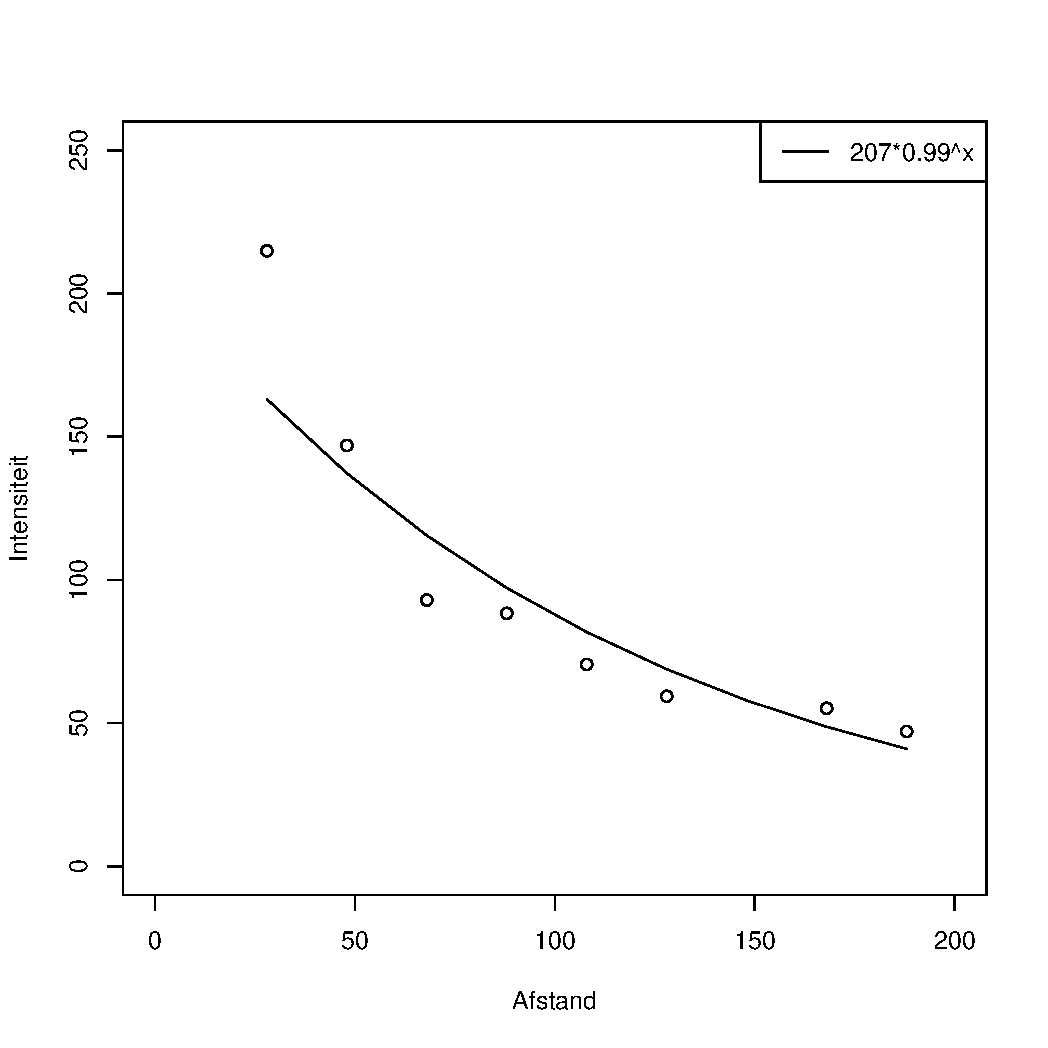
\includegraphics[width=85mm]{resources/plotIR.pdf}
  \caption{De meetwaarden van de IR-sensor volgens een bepaalde afstand}
  \label{fig:plotIR}
\end{figure}

\begin{figure}
\begin{center}
 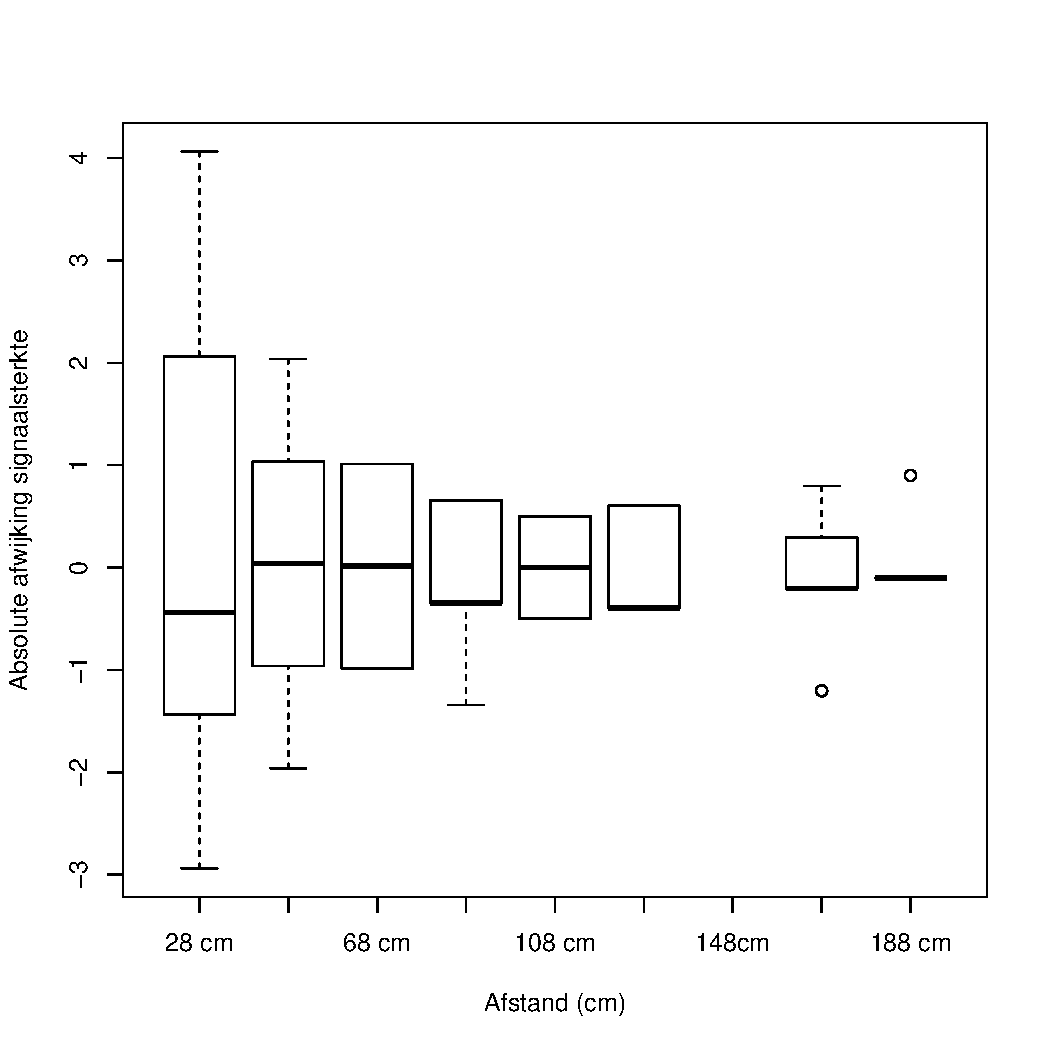
\includegraphics[width=85mm]{./resources/bloxplotIR.pdf}
 \caption{Sensorwaarden van de IR-sensor bij verschillende afstanden}
 \label{fig:boxplotIR}
\end{center}
\end{figure}

Uit testen blijkt dat een significante hoeveelheid van het IR licht via weerkaatsingen door de infraroodsensor gedetecteerd wordt.
De sterkte is bij weerkaatsing herkenbaar lager dan bij een rechtstreekse detectie (zie grafiek \ref{fig:boxplotSpiegeling}).  Men kan dus eventueel ook aan de hand van de signaalsterkte herkennen of de Pac-Man zich bvb. achter een hoek bevindt. In dit geval kan deze meting zelfs best genegeerd worden. Het reconstrueren van een weerkaatsingpatroon is een zeer moeilijke opgave.

\begin{figure}
\begin{center}
 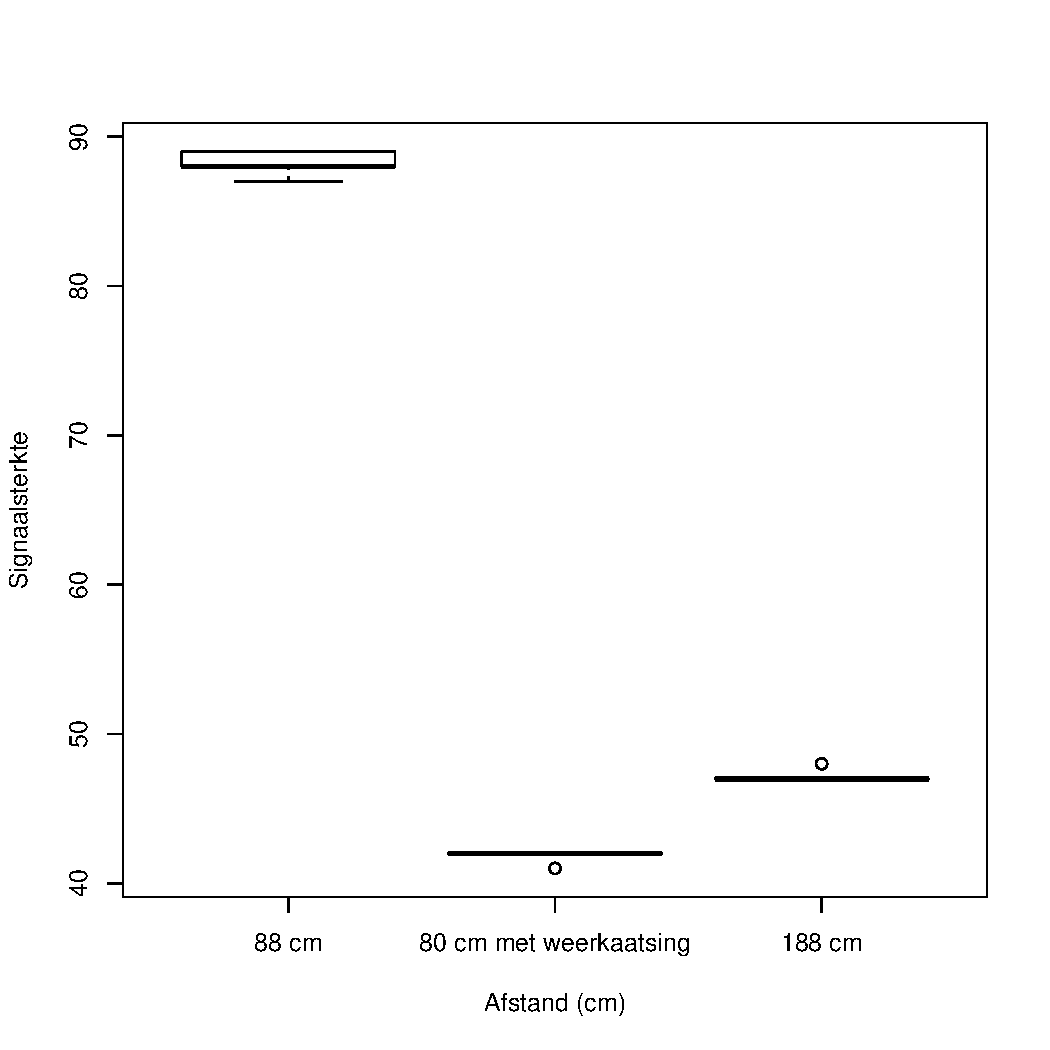
\includegraphics[width=85mm]{./resources/boxplotSpiegeling.pdf}
 \caption{Sensorwaarden van de IR-sensor bij weerkaatsing en verschillende afstanden}
 \label{fig:boxplotSpiegeling}
\end{center}
\end{figure}

Een nadeel van zo'n filtering is dat deze de afstand waarop geschat kan worden inperkt. Zoals men kan zien op de grafiek \ref{fig:boxplotSpiegeling}, kunnen we geen afstanden van meer dan 160 cm (4 sectoren) onderscheiden van weerkaatsingen. Voor demo 2 en 3 zal moeten afgewogen worden wat de beste oplossing is: een grotere gemeten afstand maar misschien niet nauwkeurig, of een grotere zekerheid garanderen. Hier zal ook rekening gehouden moeten worden met de andere teams. 

\section{Demo 2}

Aangezien in demo 1 bleek dat de lichtsensor niet goed functioneerde, zullen we naar demo 2 toe de lichtsensor opnieuw van dichterbij bekijken. Het is moeilijk om de exacte condities van de demo na te bootsen, maar we kunnen wel de in de databank opgeslagen gegevens analyseren. Tevens zullen andere pistes bewandeld worden, op zoek naar een stabieler resultaat. Een eerste test zal opnieuw het plaatsten van een \emph{kapje} zijn, zoals in het eerste semester getest werd. Deze aanpak werd toen niet gebruikt vanwege de hoogteverschillen in het parcours. 

\section{Demo 3}

Aangezien afgesproken werd in de commissie om de robots te voorzien van een vlaggetje waarop hun kleur bekend gemaakt wordt, werd dit aan de onze robot bevestigd. Verder werden er geen aanpassingen meer doorgevoerd, aangezien de lichtsensor bij demo 2 werkte naar verwachting.

\chapter{Strategie}

Aangezien wij ons slechts sinds enkele maanden begeven op het terrein van autonome robots en artifici\"ele intelligentie, zou het dom zijn te veronderstellen dat er ons nog niemand is voor gegaan. We hebben daarom een literatuurstudie rond de concepten van Pac-Man en autonome \emph{ghosts} gedaan.

We vonden een paper omtrent \emph{Collaborate Diffusion} \cite{Repenning06}. Hierin wordt voorgesteld om een vorm van \emph{Hill Climbing} toe te passen om zo verschillende autonome \emph{ghosts} toe te laten samen te werken om een Pac-Man te achtervolgen. Hierbij hebben zij geen nood aan bijkomende onderlinge communicatie naast de informatie over de omgeving.

Ondanks het feit dat we geen overeenstemming met de andere teams konden bereiken om allen dit algoritme te implementeren, blijft het een zeer interessant algoritme om toe te passen voor het bepalen van ons eigen pad.

\section{Achtervolgstrategie}

Wanneer de Pac-Man gezien wordt, stuurt deze een \emph{geur} uit. Deze plant zich langs gekende sectoren voort. Dit wordt gedaan door het gemiddelde van de 4 omliggende sectoren te berekenen, indien er een muur staat is de waarde 0. Zo ontstaat er een \emph{hoogte-kaart} met aan de top een Pac-Man. De \emph{ghosts} kunnen nu aan de hand van een eenvoudig \emph{Hill Climbing} algoritme een optimale weg volgen naar de Pac-Man.

Wanneer een \emph{ghost} de Pac-Man opmerkt, kan deze positie op de kaart een zeer hoge waarde gegeven worden. Deze kaart wordt vaak herberekend en de geur van een Pac-Man zal dus snel verdwijnen. En dit is zoals het in de realiteit ook zal zijn. De Pac-Man beweegt zich doorheen het doolhof en zal niet op \'e\'en plek blijven wachten. Als een Pac-Man meerdere keren gezien wordt, zal zijn positie ook een constantere \emph{geur} verspreiden, waardoor de \emph{ghosts} van alle kanten op hem kunnen naderen. 

Een handige manier om de geur van een Pac-Man te visualiseren is door middel van een kleurenpallet. We hebben hierbij gekozen voor het kleurenpallet zoals dit in de natuur voorkomt. Figuur \ref{fig:colormap} toont dit kleurenpallet met een aanduiding van de overeenkomstige interne numerieke waarde die aan een sector toegekend wordt om de intensiteit van de \emph{geur} voor te stellen.

\begin{figure}[htbp]
  \centering
  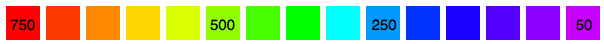
\includegraphics[width=150mm]{resources/colormap.png}
  \caption{Kleuren en voorgestelde interne \emph{geur}-waarden}
  \label{fig:colormap}
\end{figure}

Figuur \ref{fig:hillclimbing1} toont een uitgangssituatie met een Pac-Man die een een uitdijende \emph{geur} verspreidt.

\begin{figure}[htbp]
  \centering
  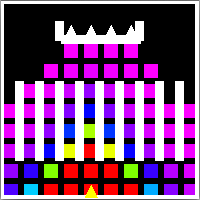
\includegraphics[width=50mm]{resources/hillclimbing1.png}
  \caption{Hill Climbing}
  \label{fig:hillclimbing1}
\end{figure}

Om te voorkomen dat \emph{ghosts} allemaal dezelfde weg volgen en enkel achter Pac-Man lopen slorpt iedere \emph{ghost} de geur op door de waarde van zijn huidige sector op 0 te zetten. Hierdoor ontstaat er een dal rond iedere \emph{ghost} en zullen de anderen een omweg zoeken. Dit zorgt er ook voor dat de \emph{ghosts} elkaar van nature uit ontwijken en niet zullen botsen. Figuur \ref{fig:hillclimbing2} illustreert dat, eens een \emph{ghost} een bepaalde \emph{beste} route naar de Pac-Man heeft ingeslagen, het pad achter hem minder interessant wordt voor de overige achtervolgers. In de voorstelling ontstaat er een \emph{deuk} in de \emph{geur} achter de \emph{ghost}. Andere \emph{ghosts} zullen daarom eerder andere paden, parallel aan het reeds ingeslagen pad, kiezen.

\begin{figure}[htbp]
  \centering
  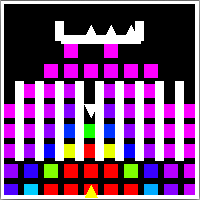
\includegraphics[width=50mm]{resources/hillclimbing2.png}
  \caption{Hill Climbing met afsluiting van pad}
  \label{fig:hillclimbing2}
\end{figure}

\section{Verkenstrategie}

De verkenstrategie is gebaseerd op hetzelfde principe. Hier is er niet \'e\'en bron die een geur uitstuurt, maar iedere onbekende sector stuurt een geur uit. De robot zal hierdoor altijd naar het dichtstbijzijnde en het meest onverkende stuk van het doolhof willen gaan. Daarnaast zorgt dit principe er ook voor dat een robot zal terugkeren op zijn stappen en automatisch terugkeert naar achtergelaten onbekende sectoren. We kunnen stellen dat het algoritme impliciet \emph{Depth-First-Search} implementeert. Figuur \ref{fig:dfs} toont een robot die een onbekend doolhof aan het verkennen is. De felgroene sectoren zijn onbekende sectoren en hebben een hogere waarde dan de reeds bezochte sectoren.

\begin{figure}[htbp]
  \centering
  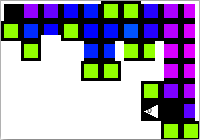
\includegraphics[width=50mm]{resources/dfs.png}
  \caption{Hill Climbing met impliciet \emph{Depth-First-Search} zoekgedrag}
  \label{fig:dfs}
\end{figure}

Het toepassen van hetzelfde algoritme voor beide deelproblemen, levert ons in essentie een enkelvoudige implementatie van beide. Door het toekennen van goed gekozen waarden aan onbekende sectoren en aan sectoren waar Pac-Man werd gezien, stelt het algoritme ons in staat om steeds het optimale doel te kiezen. Wanneer er zich geen pad bevindt naar de Pac-Man zal een \emph{ghost} onbekende sectoren trachten te verkennen. Wanneer er een pad bestaat naar de Pac-Man zal zijn \emph{geur} dit pad nog extra versterken en zal een \emph{ghost} automatisch hierdoor aangetrokken worden.

\section{Samenwerking en onzekerheid}

De informatie die van de verschillende robots verzameld wordt is zeker niet perfect. We moeten hiermee rekening houden, zonder parano\"ide te worden en alle informatie te weigeren. We hanteren in de encodering van de informatie over het doolhof een gelaagd principe: enerzijds houden we bij of we ergens een muur hebben waargenomen of niet. Maar daarnaast houden we ook bij of we iets weten over die muur of niet. Zo ontstaan er drie mogelijk statussen waarin een muur zich kan bevinden: \emph{onbekend}, \emph{geen muur} en \emph{wel een muur}.

Aan de hand van deze statussen kunnen we nu overgangen gaan defini\"eren die we aanvaardbaar vinden. Een \emph{onbekende} muur kan zonder problemen omgezet worden in \emph{geen muur} of \emph{wel een muur}. Wanneer we echter over informatie beschikken over een muur en we krijgen informatie die tegenstrijdig is, dan zullen we de status van de muur terug naar \emph{onbekend} brengen.

De gevolgen voor het \emph{Collaborate Diffusion} algoritme kunnen inhouden dat een sector die volledig gekend was en die dus geen \emph{geur} meer uitstraalde, plots opnieuw een waarde krijgt die zich door het doolhof zal verspreiden. Hierdoor zal de robot geneigd zijn om deze opnieuw te gaan verkennen.

\section{Effectiviteit}

Het \emph{Collaborate Diffusion} algoritme werkt optimaal indien alle achtervolgende robots dezelfde implementatie en parameters gebruiken. Ofschoon dit niet het geval is in onze situatie kan het toch zijn nut bewijzen voor onze robot op zich. Zo is de mogelijkheid om simultaan zowel sectoren te verkennen, als het achtervolgen van Pac-Man, een groot pluspunt voor de robuustheid van de robot.

Het \emph{collaboratie diffusion} algoritme is in essentie een implementatie van het \emph{Hill Climbing II} algoritme. Dit zorgt ervoor dat de robot ten alle tijde volgens het meest optimale pad naar de Pac-Man tracht te rijden. Mits kennis van dit algoritme is het voor de bestuurder van de Pac-Man zeker mogelijk om hiermee rekening te houden en er voordeel uit te halen. Het algoritme zal bijvoorbeeld nooit een minder optimale weg kiezen om de Pac-Man via een andere weg klem te rijden.

Dit concept is wel inherent ingebouwd indien een andere robot het meest optimale pad kiest en zo de verspreiding van de \emph{geur} tegen gaat. Op dit moment lijkt het alsof de robot een minder optimaal pad zal volgen, doch het is een pad waarlangs de \emph{geur} hem wel bereikt.

Met de mini-simulator hebben we verschillende scenario's uitgetest. Hierbij werd ook gebruik gemaakt van een bewegende Pac-Man. Buiten enkele exotische opstellingen, werd de Pac-Man toch altijd in een redelijke tijdspanne gevangen.

\chapter{Softwaredesign}

In het eerste semester hadden we reeds een redelijk uitgebreid raamwerk opgebouwd om robots samen te stellen uit componenten. Dankzij dit werk kunnen we in het tweede semester hier op verder bouwen door de bestaande concepten verder te verfijnen en uit te breiden.

Echter, vooraleer de definitieve beslissing genomen werd om ver te bouwen op de bestaande architectuur, werden enkele andere opties bekeken. Enerzijds werd de bestaande \emph{Pilot} klasse van de Lejos software bekeken en anderzijds werd in literatuur gezocht naar andere mogelijke opstellingen.

De bestaande \emph{Pilot} klasse van Lejos volgt geen radicaal verschillende aanpak. Wel hebben we het \emph{behaviour} idee ge\"incorporeerd in ons eigen ontwerp. Bij onze zoektocht in de literatuur moesten we tot het besluit komen dat er waarschijnlijk evenveel mogelijke ontwerpen zijn als er robots zijn. Veel van de bekeken oplossingen begeven zich deels op het vlak van Lejos of belichten een veel hoger niveau. Een concrete, de facto, alternatieve architectuur voor het aansturen van een robot werd niet gevonden. Wel hebben we veel idee\"en opgedaan die verwerkt werden tijdens de verschillende bijwerkingen van de software.

De architectuur van het eerste semester heeft zich bewezen. De structuur en concepten zijn gekend, alsook de problemen en tekortkomingen. Alles in beschouwing genomen werd unaniem besloten om verder te werken op het bestaande design en elementen uit de studie van andere oplossingen op te nemen waar nuttig.

\section{Robot}

Het klasse diagram op figuur \ref{uml:design-semester1} toont de belangrijkste bouwstenen van ons robot-raamwerk, zoals dit tijdens het eerste semester werd ontworpen: een \emph{Robot}-entiteit beschikt over een \emph{RobotAPI} om met de fysieke robot informatie uit te wisselen. Deze informatie heeft betrekking op de gemeten waarden van de verschillende sensoren als ook het instellen van de motoren. De \emph{RobotAPI} stelt ons in staat om door het vervangen van \'e\'en enkele klasse, identiek dezelfde \emph{Robot}-entiteit te gebruiken in een echte fysieke robot, alsook in een gesimuleerde wereld.

\begin{figure}[htbp]
  \centering
  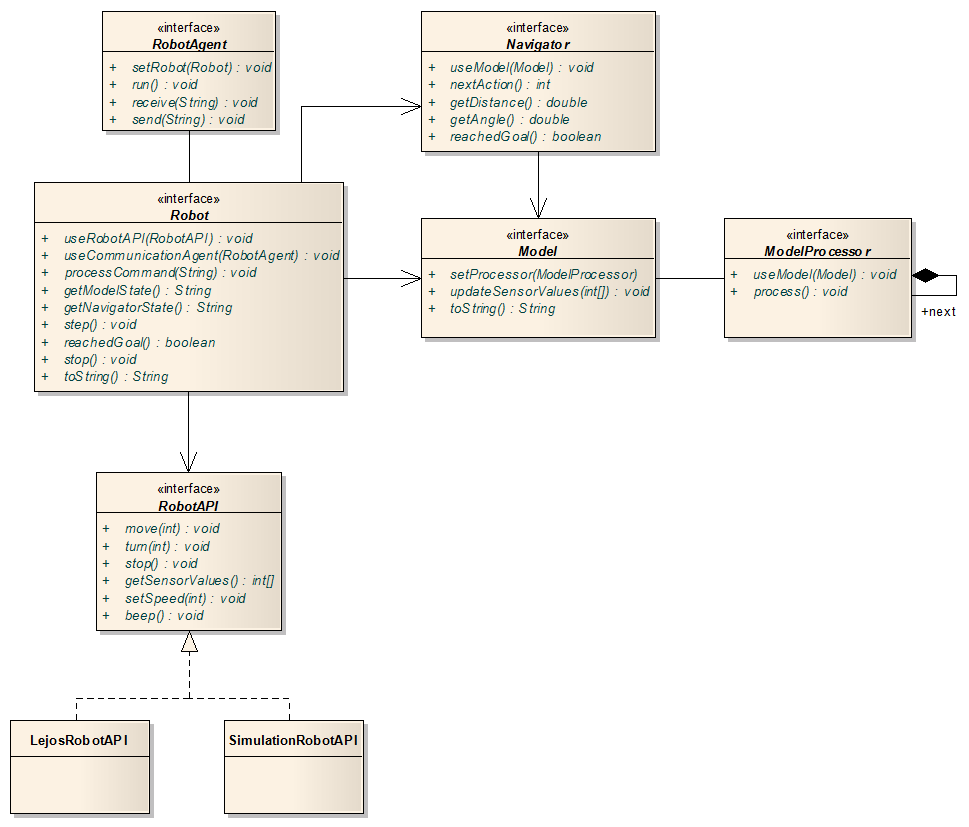
\includegraphics[width=110mm]{resources/design-semester1.png}
  \caption{Design $1^e$ semester}
  \label{uml:design-semester1}
\end{figure}

De \emph{Robot} beschikt verder over een \emph{Model} waarin alle informatie uit de wereld wordt samengebracht. Dit \emph{Model} kan verrijkt of bijgewerkt worden door zgn. \emph{ModelProcessors}. Deze onderzoeken bepaalde delen van het \emph{Model} en trachten hieruit informatie van een hoger niveau te distilleren. Voorbeelden hiervan zijn processors die op basis van metingen door de sonar-sensor bepalen waar er zich muren bevinden.

Tot slot heeft de \emph{Robot} ook een \emph{Navigator} die op basis van de informatie in het \emph{Model} bepaalt waarheen de \emph{Robot} dient te rijden. De navigator geeft zeer basische instructies aan de \emph{Robot}, in de vorm van \emph{beweeg voor- of achterwaarts} en \emph{draai zoveel graden}.

Om met de \emph{Robot} te kunnen communiceren is een \emph{RobotAgent} voorzien, waarlangs berichten kunnen verzonden en ontvangen worden.

Het is duidelijk dat dit raamwerk een sterk herbruikbare basis biedt om verschillende robots te bouwen. Dit heeft al tijdens het eerste semester zijn nut bewezen, maar komt nog sterker naar voor bij aanvang van het tweede semester. Door het maken van een nieuwe specifieke \emph{Navigator} en bijhorend \emph{Model} met \emph{Modelprocessors}, kunnen we opnieuw een robot samenstellen, waarbij we maximaal gebruik maken van de bestaande software.

\subsection{Driver}

Ofschoon we een nieuwe \emph{Navigator} zouden kunnen maken die perfect zou passen, werd snel duidelijk dat er een verfijning van het raamwerk mogelijk was: daar waar tijdens het eerste semester de robot geen resolutie had bij het rijden, is dit in het tweede semester wel het geval. Door het introduceren van het concept van sectoren is er een duidelijk onderscheid tussen het operationele en strategische aspect van het besturen van de robot. Operationeel dient de robot optimaal van sector naar sector te rijden, zodat op strategisch niveau kan geredeneerd worden in termen van deze sectoren.

De functionaliteit om van sector naar sector te rijden zou typisch terecht gekomen zijn in een \emph{Navigator}-implementatie. Deze wordt in het verfijnde raamwerk ondergebracht in een zgn. \emph{Driver}. Het klasse diagram op figuur \ref{uml:design-semster2} toont dat de introductie van de Driver letterlijk een uitbreiding is van het bestaande raamwerk. Voor het tweede semester is er tevens een eerste implementatie van de Driver gemaakt in de vorm van een \emph{ManhattanDriver}.\footnote{Zo genoemd naar analogie met Manhattan Distance en de Taxicab geometrie.} 

\begin{figure}[htbp]
  \centering
  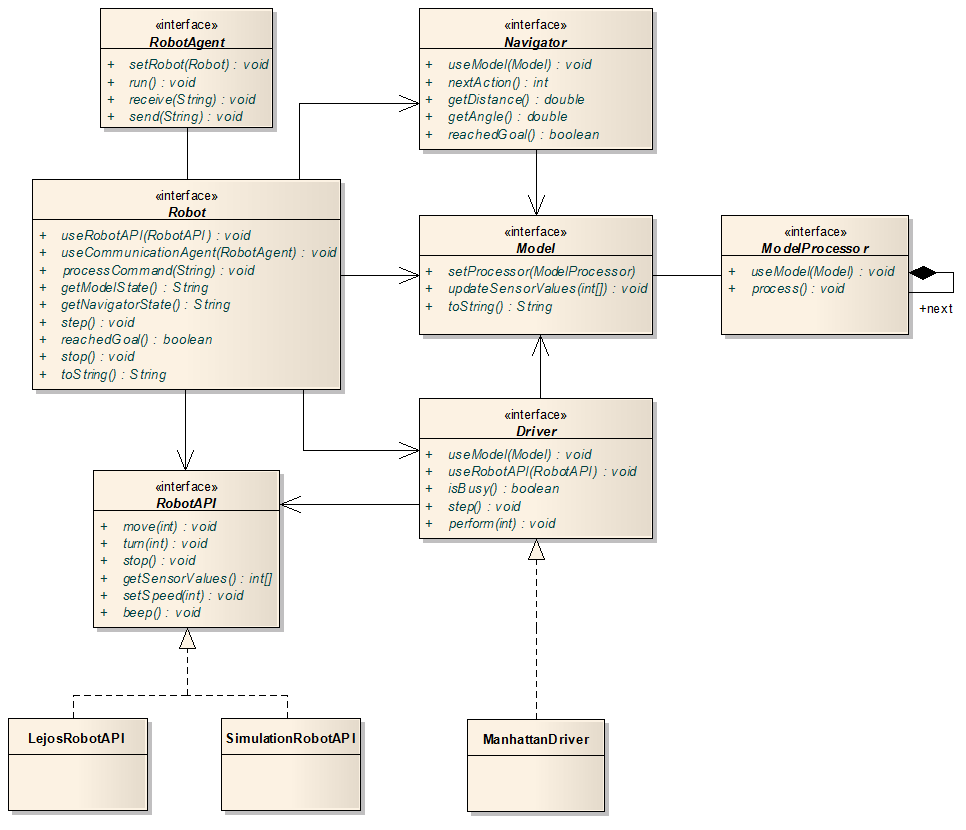
\includegraphics[width=110mm]{resources/design-semester2.png}
  \caption{Design $2^e$ semester}
  \label{uml:design-semster2}
\end{figure}

\subsection{Grids en Sectoren}

De \emph{Navigator} kan zich nu specifiek toeleggen op het bepalen van de volgende \emph{Sector}, waarheen de Driver moet rijden. Om deze taak te ondersteunen werden de concepten \emph{Grid}, \emph{Sector} en Agent in het leven geroepen. Het klasse diagram op figuur \ref{uml:grids-sectoren} geeft een overzicht van hun samenhang en van de effectieve implementaties die samen de zgn. \emph{GhostRobot} opbouwen.

\begin{figure}[htbp]
  \centering
  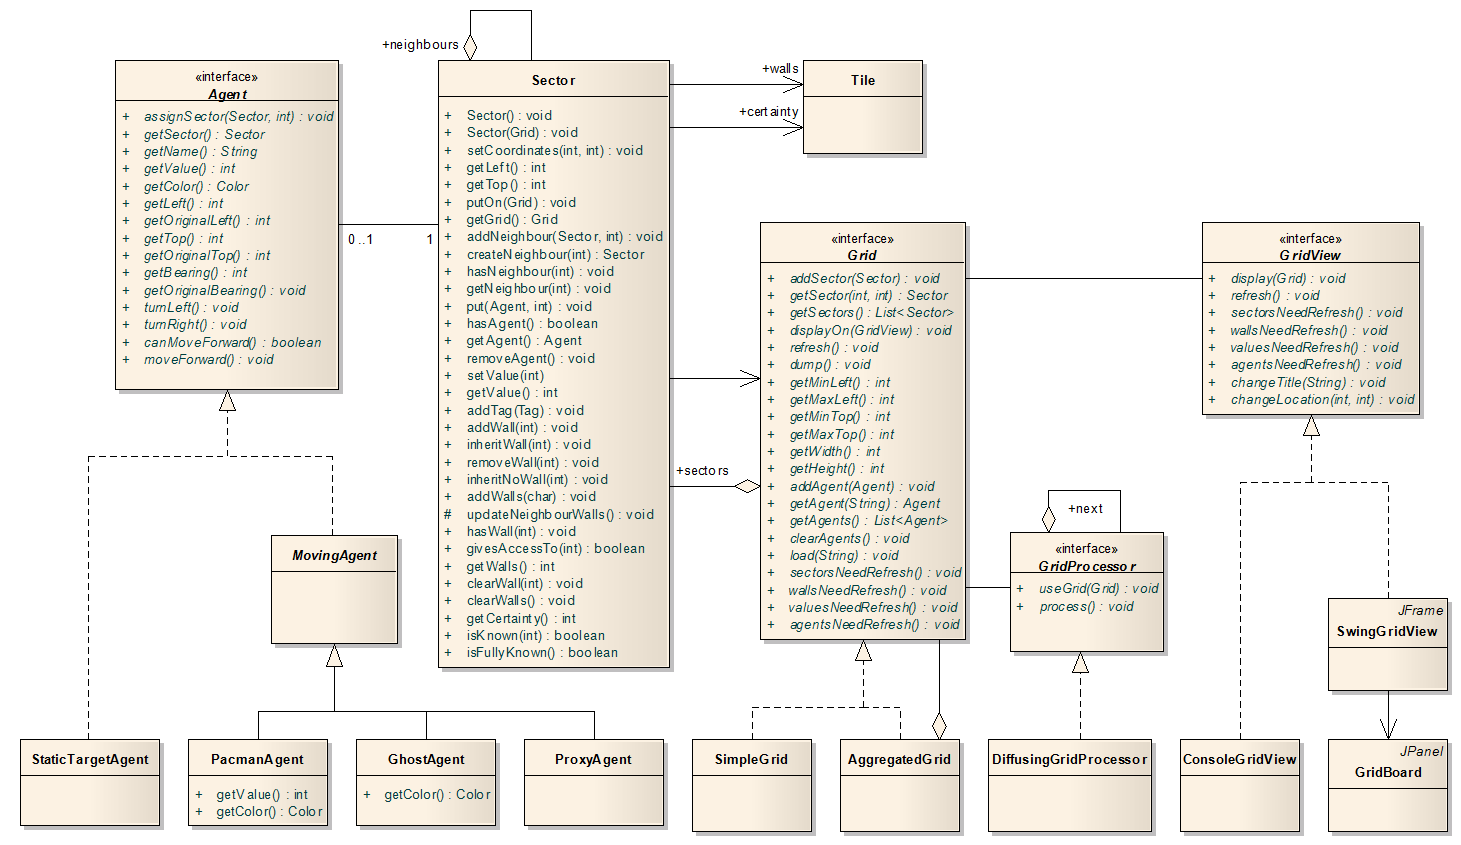
\includegraphics[width=200mm, angle=90]{resources/grids-sectors.png}
  \caption{Design Grids en Sectoren}
  \label{uml:grids-sectoren}
\end{figure}

Centraal staat het concept van de \emph{Sector} in een \emph{Grid}. Een \emph{Sector} heeft een co\"ordinaat relatief t.o.v.\ de \emph{Grid} waarop het zich bevindt, heeft potentieel 4 muren, elk al dan niet gekend, heeft een waarde en kan bezet worden door een Agent. De waarde van een \emph{Sector} zal gebruikt worden om de hoogte of de intensiteit van de geur weer te geven. Een Agent kan zich doorheen de \emph{Grid} bewegen langs de sectoren. De meeste functionaliteit van een Agent is ge\"implementeerd in een abstract basis klasse, MovingAgent. Mits kleine configuratieaanpassingen, implementeren de \emph{PacmanAgent} en \emph{GhostAgent} zo de agents die op de \emph{Grid} voorkomen. Een \emph{ProxyAgent} werd gebruikt om in een simulator een echte \emph{Agent} voor te stellen die de volledige \emph{Grid} nog niet kent en de \emph{StaticTargetAgent} werd speciaal voorzien voor de voorbereiding van de eerste demo.

Optioneel kan aan een \emph{Grid} ook een \emph{GridView} gegeven worden. Deze voorziet een visualisatie van de \emph{Grid} en kan op verschillende manieren ingevuld worden. Voor dit project hebben we twee implementaties gemaakt: enerzijds een \emph{ConsoleGridView} die gedetailleerde informatie over de sectoren weergeeft en een \emph{SwingGridView} die een grafische voorstelling geeft van de \emph{Grid}. Deze laatste wordt gebruikt voor de visualisatie in o.a. de simulator.

Een \emph{Grid} beschikt ook over een \emph{GridProcessor}. Net zoals de \emph{ModelProcessor} kan dit een geschakelde lijst van processoren zijn die de \emph{Grid} kunnen ondervragen en bijwerken. Zo hebben we een \emph{DiffusionGridProcessor} ge\"implementeerd die de waarde van de sectoren zal bijwerken volgens het eerder beschreven algoritme.

De nieuwe robot zal ook informatie van andere robots ontvangen. Deze worden allemaal opgeslagen in een zelfde \emph{Grid}. Een tweede implementatie van het \emph{Grid} concept, de zgn. \emph{AggregatedGrid}, is in staat om een aantal verschillende grids samen in beschouwing te nemen en de \emph{som} van deze als een geaggregeerd beeld aan te bieden.

\subsection{GhostRobot}

Het klasse diagram op figuur \ref{uml:ghostrobot} geeft tot slot de volledige compositie van de nieuwe \emph{GhostRobot} weer. De \emph{GhostRobot} beschikt over een \emph{GhostModel}, \emph{GhostNavigator} en \emph{GhostDriver}.

\begin{figure}[htbp]
  \centering
  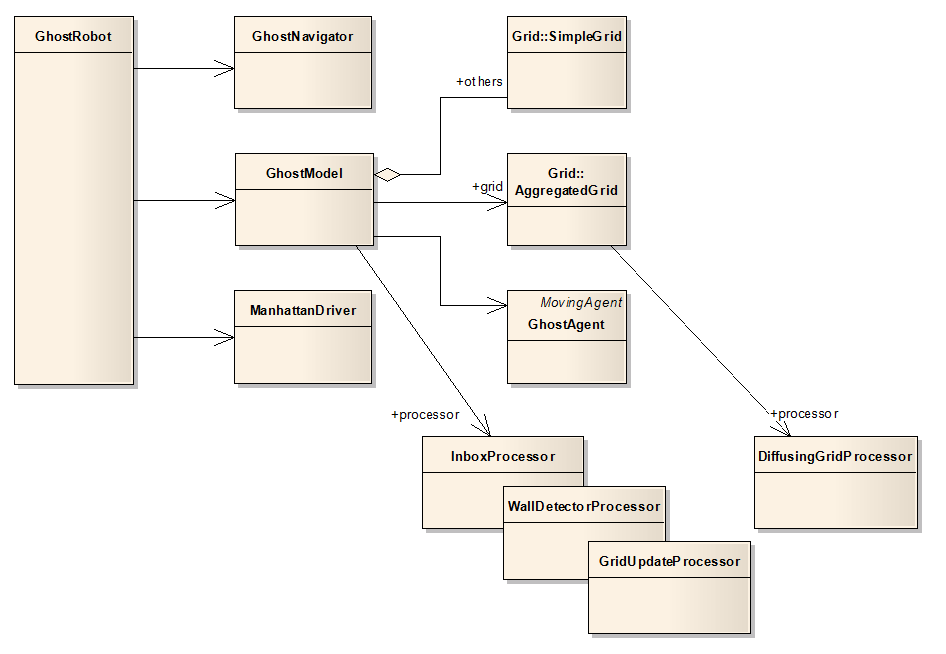
\includegraphics[width=110mm]{resources/ghostrobot.png}
  \caption{Compositie GhostRobot}
  \label{uml:ghostrobot}
\end{figure}

Het \emph{GhostModel} bevat \emph{Grids} voor elk van de andere robots alsook een \emph{AggregatedGrid} voor de eigen Agent. Zolang er geen gemeenschappelijk referentiepunt\footnote{Referentiepunten worden op het parcours voorgesteld door geori\"enteerde barcodes.} is gevonden zijn de verschillende \emph{Grids} niet met elkaar in verband te brengen. Wanneer er echter een gemeenschappelijk referentiepunt gevonden is, kan de corresponderende \emph{Grid} van de andere robot toegevoegd worden aan de eigen \emph{AggregatedGrid}, waardoor de informatie van beide \emph{Grids} gecombineerd wordt en een ruimer wereldbeeld beschikbaar wordt.

De eigen \emph{AggregatedGrid} beschikt ook over een \emph{DiffusingGridProcessor} die het algoritme voor het bepalen van de waarde van een \emph{Sector} zal toepassen op de \emph{AggregatedGrid}, waardoor de \emph{GhostNavigator} een redelijk eenvoudige beslissing kan nemen op basis van de waarden van de vier aangrenzende sectoren.

Het \emph{GhostModel} is verder voorzien van een aantal \emph{ModelProcessoren} die de inkomende informatie verwerken tot informatie waarmee de \emph{GhostNavigator} beslissingen kan nemen. Enerzijds is er een InboxProcessor die de binnenkomende berichten van de andere robots omzet in aanpassingen aan de verschillende \emph{Grids} in het \emph{GhostModel}. Anderzijds is er de \emph{WallDetectorProcessor} die op basis van de gemeten waarden door de sonar-sensor een beeld zal samenstellen van de huidige \emph{Sector}. Tot slot is er de \emph{GridUpdateProcessor} die de nieuwe muurinformatie zal verwerken in de eigen \emph{Grid} en eventueel nieuwe sectoren zal toevoegen.\footnote{Naast deze drie \emph{ModelProcessoren} zijn er nog andere actief. Het betreft hier bvb. de \emph{LineModelProcessor} of de \emph{WallDetectionModelProcessor}. Deze zorgen voor informatie die door de \emph{Driver} zal gebruikt worden om optimaal naar de volgende sector te rijden. Veel van deze \emph{ModelProcessoren} maakten reeds deel uit van de robots uit het eerste semester.}

\subsection{Performantie}
\label{sect:performance}

Met de expliciete keuze om alle software op de robot zelf te implementeren, zijn we natuurlijk gebonden aan de beperkingen van de robot. Enerzijds heeft deze geen processor die te vergelijken is met de processors van hedendaagse computers. Dit is echter voor onze architectuur en gekozen zoekstrategie geen probleem. Door gebruik te maken van een zeer eenvoudig \emph{local Hill Climbing} algoritme, gebaseerd op het principe van \emph{Collaborate Diffusion}, vragen we zeer weinig van de processor. We slagen er in om een \emph{frame rate} te bekomen die rond de 80 FPS \footnote{Frames Per Second is een term die uit de grafische sector komt en weergeeft hoeveel beelden per seconde gemaakt worden, maar wordt ook gebruikt in andere contexten. Een \emph{frame} is dan het geheel van taken. Voor onze robot bestaat \'e\'en frame uit het opvragen van de sensorwaarden, het bijwerken van het \emph{Model}, het kiezen van een volgende actie en het initi\"eren van de uitvoering.} ligt, wat betekent dat de frequentie waarmee de robot al zijn taken uitvoert meer dan hoog genoeg is voor de taken die moeten uitgevoerd worden. Proefondervindelijk hebben we vastgesteld dat een frame rate van 60 FPS een minimum is om de verschillende taken naar behoren uit te voeren.

\subsubsection{Geheugengebruik}

Het aspect geheugen is dan weer wel een sterk beperkende factor. De robot beschikt slechts over een werkgeheugen van 64KB waarvan een deel reeds wordt ingenomen door het geladen programma. Tijdens het eerste semester was de hoeveelheid informatie die opgeslagen werd in het \emph{Model} nagenoeg constant, of had ten minste een gekende bovengrens. In het tweede semester moeten we echter informatie bijhouden over het speelveld waarop we ons bewegen. Aangezien we op voorhand niet weten hoe groot dit speelveld is kunnen we niet op voorhand een bovengrens bepalen voor het geheugen nodig om deze informatie op te slagen. Daarbij komt dat we dit speelveld niet alleen moeten bijhouden voor onze eigen robot, maar ook voor de drie andere robots.

Intern stellen we het speelveld of \emph{Map} voor als een verzameling sectoren, die verbonden zijn met elkaar door bi-directionele verwijzingen. Telkens een robot een nieuwe sector \emph{ontdekt} wordt er intern ook een nieuw \emph{Sector} object aangemaakt. De grootte van zo'n \emph{Sector} object is dus bepalend voor de hoeveelheid sectoren we maximaal kunnen bijhouden in het geheugen van de robot.

Vlak voor demo 1, was een \emph{Sector} ongeveer 370 bytes groot en konden we ongeveer 145 sectoren opslaan in ons geheugen. In een worst-case scenario betekent dit dat we per robot 36 sectoren konden opslaan, wat overeenkomt met een speelveld van 6 bij 6. We hebben vervolgens twee pistes gestart om dit probleem aan te pakken. Enerzijds hebben we het geheugengebruik van de \emph{Sector} klasse aangepakt en gereduceerd tot 280 bytes. Anderzijds hebben we besloten om binnenkomende informatie van andere robots slechts te bewaren totdat deze informatie op basis van een barcode kon ge\"importeerd worden in de \emph{Map} van de eigen robot. Op dat ogenblik gooien we de Map van de andere robot weg en voegen de nog volgende binnenkomende informatie rechtstreeks toe aan onze eigen \emph{Map}.

Op deze manier zal er een trapsgewijs verval zijn van het totale aantal sectoren die moeten bijgehouden worden. Immers wanneer alle robots een gemeenschappelijke barcode hebben gevonden, zal er slechts \'e\'en \emph{Map} overblijven, nl. die van de eigen robot.

Met deze aanpassingen konden we voor demo 1 een maximaal aantal van 200 sectoren opslaan, ofwel 50 per robot, wat overeenkomt met een speelveld van 7 bij 7. Rekening houdend dat deze situatie zich niet kan voordoen, omdat de robots nooit allemaal afzonderlijk het hele speelveld moeten ontdekken en sowieso gemeenschappelijke barcodes zullen tegenkomen, ligt de bovengrens voor de dimensies van het speelveld in realiteit hoger. Simulaties wezen uit dat we met 200 sectoren in staat waren om een (realistisch) speelveld van 10 bij 10 zonder problemen te kunnen verkennen met vier robots.

We hebben deze simulaties gedaan aan de hand van de mini-simulator (zie sectie \ref{sect:mini-simulator}). Wanneer 4 robots een speelveld van 10 bij 10 verkennen, zonder gebruik te maken van barcodes om informatie uit te wisselen, dan zal het totaal aantal sectoren in het geheugen van onze robot oplopen tot 400. Figuur \ref{chart:sectors-no-merge} toont een grafiek die het verloop van zo'n sessie weergeeft.

\begin{figure}[htbp]
  \centering
  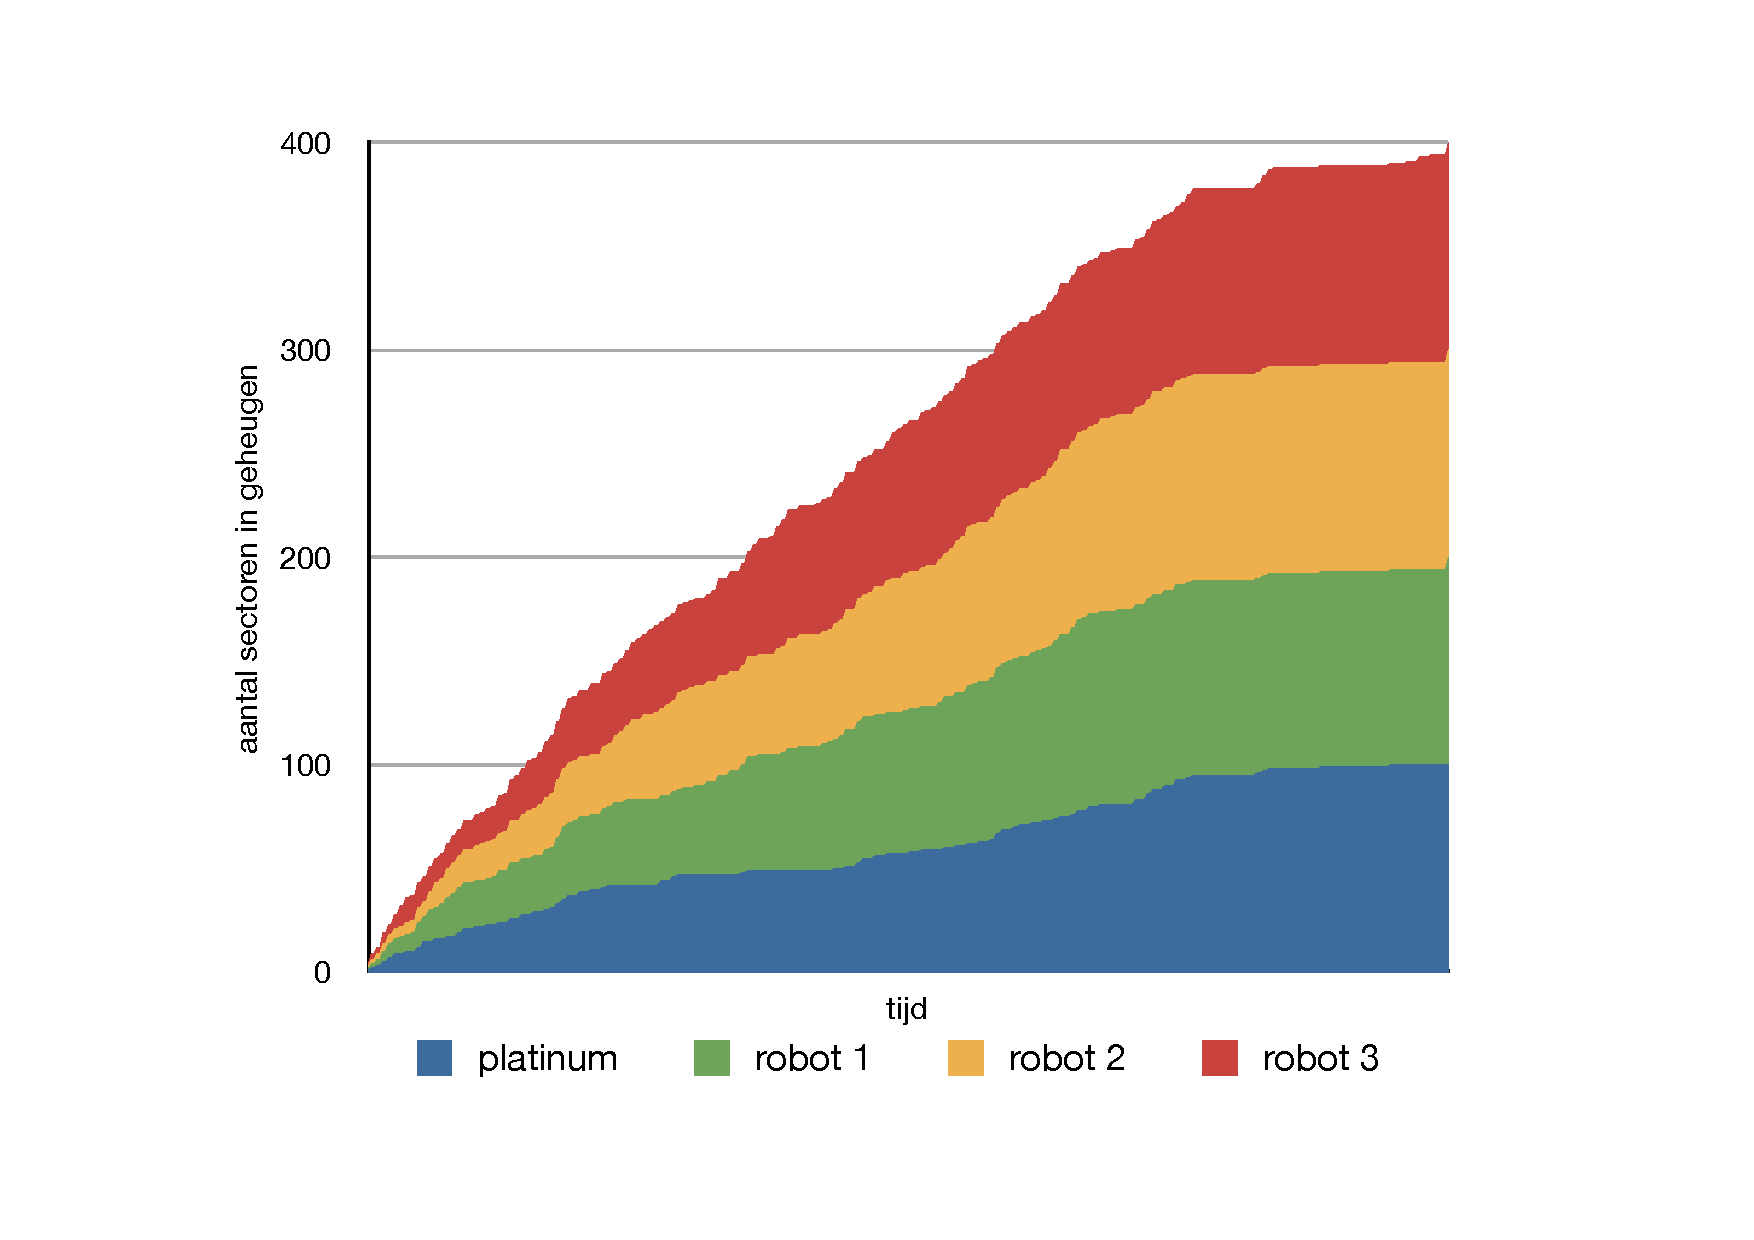
\includegraphics[width=100mm]{resources/sectors-no-merge.pdf}
  \caption{Verloop van het aantal sectoren zonder uitwisseling van informatie.}
  \label{chart:sectors-no-merge}
\end{figure}

Figuur \ref{chart:sectors-with-merge} toont vervolgens het resultaat van dezelfde simulatie, echter nu zal onze robot de door andere robots verkende sectoren importeren in zijn eigen map, de \emph{Map} van de andere robot uit zijn geheugen verwijderen en alle volgende nieuwe informatie rechtstreeks toepassen op zijn eigen \emph{Map}.

\begin{figure}[htbp]
  \centering
  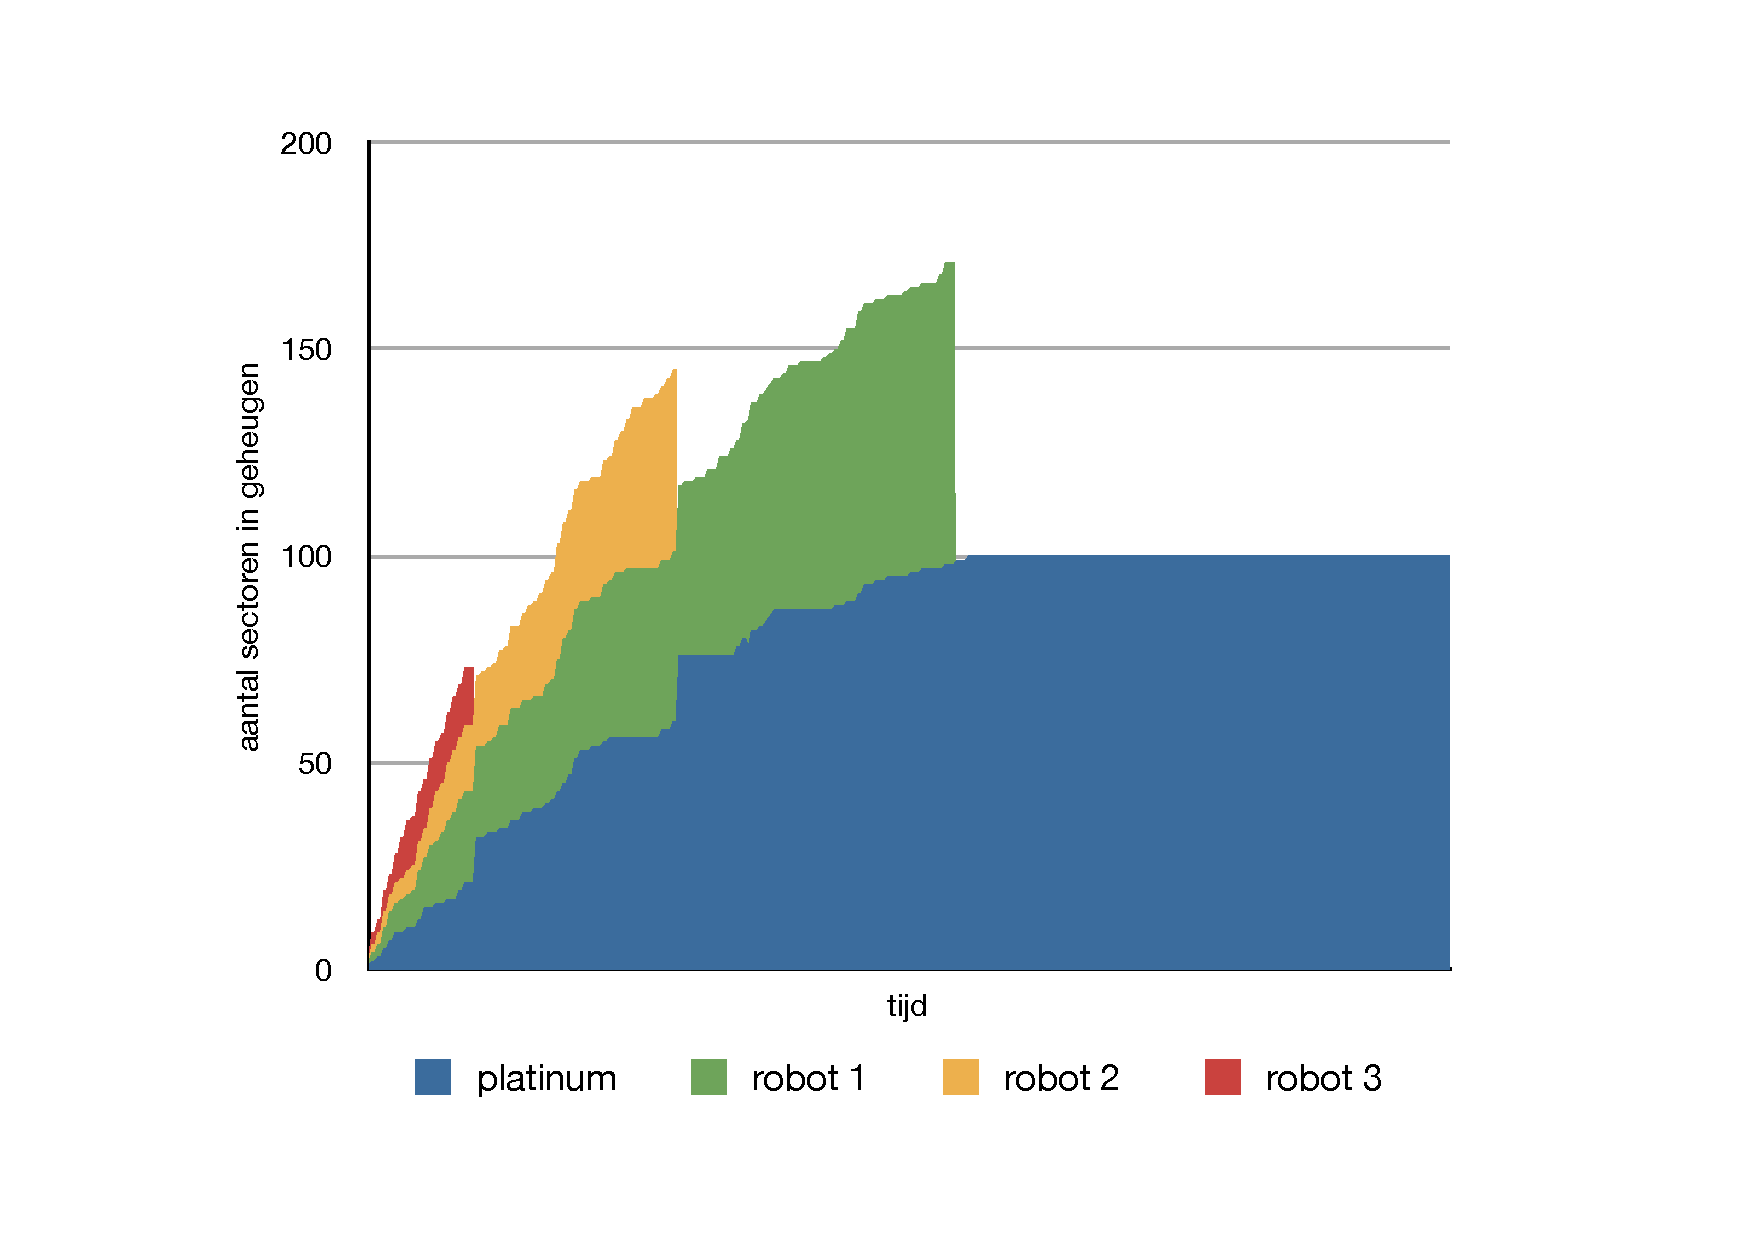
\includegraphics[width=100mm]{resources/sectors-with-merge.pdf}
  \caption{Verloop van het aantal sectoren met uitwisseling van informatie.}
  \label{chart:sectors-with-merge}
\end{figure}

We zien hier duidelijk twee zaken naar voor komen: enerzijds beschikt de robot veel sneller over informatie van het hele speelveld en anderzijds wordt het totale geheugengebruik ook drastisch beperkt.

Deze aanpak heeft natuurlijk een groot nadeel. Eens de gegevens van een andere robot ge\"importeerd zijn, is het niet mogelijk om deze terug te verwijderen. De architectuur voorziet een \emph{AggregatedGrid} die de gegevens van de echte \emph{Grids} dynamisch aggregeert. Hierbij moeten de \emph{Grids}  van de verschillende robots echter wel in het geheugen bewaard blijven.

Met het oog op demo 2 en 3 willen we nog verdere optimalisaties doorvoeren op het vlak van het geheugengebruik van een \emph{Sector}. Anderzijds onderzoeken we een oplossing waarbij er sectoren uit de verschillende mappen van andere robots verwijderd worden in functie van het nog beschikbare geheugen.

\section{PC}

Op het vlak van de PC kunnen we opnieuw verder bouwen op onze bestaande \emph{ServiceAgent}. Naast het logging-kanaal, zal deze nu ook een tweede Bluetooth kanaal volgen, langs het welke de boodschappen van het \emph{Ghost Protocol} kunnen uitgewisseld worden met de \emph{exchange-queue} op de RabbitMQ server.

Ook het \emph{Dashboard} wordt uitgebreid met meer informatie over de werking van het zoek-algoritme en de map-verkenning. Hiervoor moet louter bijkomende informatie vanuit het \emph{Model} en de \emph{Navigator} doorgestuurd worden, kunnen we \emph{Log4J} eenvoudig aanpassen in configuratie en voorzien we de databank van bijkomende kolommen om de nieuwe gegevens op te slaan.

Het Dashboard zelf wordt voorzien van de nodige visualisaties voor deze nieuwe informatie. Figuur \ref{fig:dashboard} toont de nieuwe samenstelling.

\begin{figure}[htbp]
  \centering
  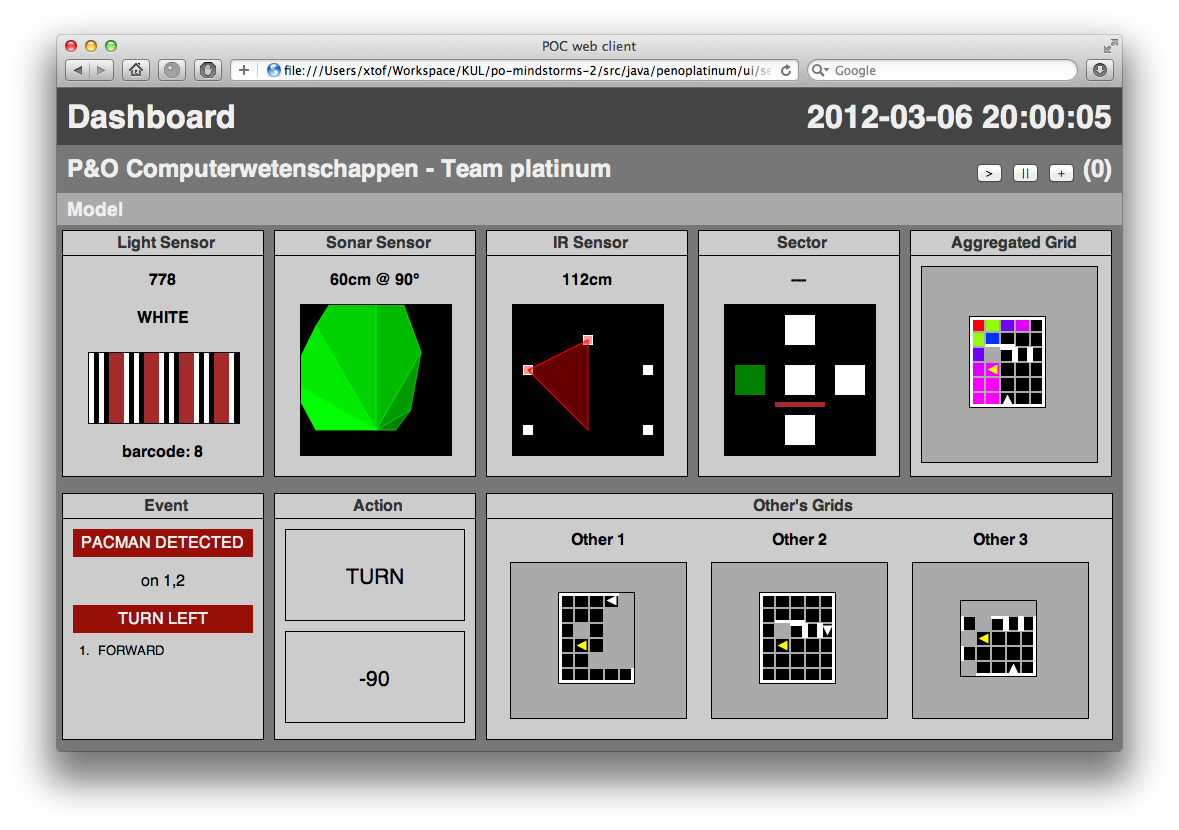
\includegraphics[width=155mm]{resources/dashboard.png}
  \caption{Nieuw Dashboard}
  \label{fig:dashboard}
\end{figure}

\subsection{Externe componenten}

We trachten bij de ontwikkeling van de software zo veel mogelijk bestaande componenten te gebruiken. Zo worden alle op de PC uitgevoerde applicaties voorzien van opties die kunnen meegegeven worden op de command line. Hierdoor worden de applicaties flexibel en kan veel van de configuratie langs deze weg dynamisch voorzien worden.

Anderzijds trachten we ook het wiel niet opnieuw uit te vinden. Het inzetten van \emph{Log4J} begon als een klassieke keuze voor een industri\"ele standaard, maar groeide gaandeweg uit tot een centrale component. Via de configuratie van \emph{Log4J} zijn we niet alleen in staat om de informatie die van de robot naar de \emph{Gateway} wordt gezonden, op te slaan in een simpele log file of in de databank. Ook de detail uitsplitsing van deze informatie naar verschillende tabellen kan ondertussen op dit niveau gebeuren. Ook werd een eigen \emph{LogAppender} gemaakt die de informatie in een bestand opslaat. Dit bestand kan vervolgens gebruikt worden door een \emph{Dashboard} zonder dat een connectie naar een server nodig is.

Zonder enige uitbreiding van de code zijn we zelfs in staat om deze informatie te posten naar bijvoorbeeld Twitter, waardoor onze robot zonder twijfel de eerste \emph{twitterende} robot is geworden. Er bestaat immers een Log4J Appender die dit voor ons doet\footnote{\url{http://code.google.com/p/twitter-log4j/}}. We moeten louter een sectie toevoegen aan de configuratie en onze robot kan gevolgd worden op Twitter: \url{https://twitter.com/\#!/RobotPlatinum}. Dus \emph{follow @RobotPlatinum}.

Een laatste belangrijke externe component is zonder twijfel \emph{Mockito}\footnote{\url{http://code.google.com/p/mockito/}}. Dit \emph{mocking framework} is de hoeksteen van een goed uitgevoerde suite aan unit testen. Van oorsprong was \emph{Mockito} echter een \emph{spying framework}, maar omdat de lijn tussen de twee verantwoordelijkheden zo dun begon te worden en meer en meer mensen gebruik wensten te maken van \emph{Mockito} is de nodige functionaliteit toegevoegd en is het op dit ogenblik \'e\'en van de beste \emph{mocking frameworks} dat beschikbaar is. De belangrijkste eigenschap van \emph{Mockito} is de laagdrempeligheid. Dit was binnen het team een belangrijke factor, omdat er weinig tot geen ervaring was hieromtrent bij de meeste van de teamleden. Dankzij deze laagdrempeligheid en de snelle \emph{return on investment} werden alle teamleden snel grote fans van dit framework.

\section{Refactoring}

Een groot deel van de tijd tussen demo 1 en 2 werd besteed aan het refactoren van de code. Aan de hand van een grondige analyse zijn verschillende historisch gegroeide pijnpunten aangeduid. Tot op dit moment was er veelal rond deze problemen gewerkt onder druk van de verschillende demo's. Met een functioneel volledig uitgewerkte oplossing, kunnen we nu zorgen dat de kwaliteit van de hele repository in lijn was met het niveau van de functionaliteit.

De belangrijkste streefdoelen waren het wegwerken van redundantie in de code, het correct benoemen van de verschillende klassen en namespaces, het toevoegen van duidelijke startpunten en het toevoegen van vele kleine extra's die het geheel tot een flexibel en gepolijst resultaat omtoveren.

Een van de grootste acties bestond er in om het sterk uitgegroeide Model op te splitsen in functionele deelmodellen en het verplaatsen van functionaliteit uit deze gegevensdragers naar de ModelProcessors. Figuur \ref{uml:refactoring} illustreert deze aanpassing.

\begin{figure}[htbp]
  \centering
  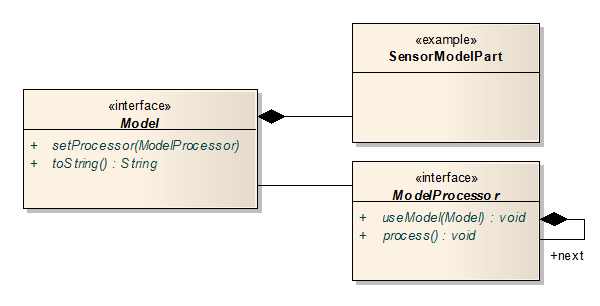
\includegraphics[width=110mm]{resources/refactoring-model.png}
  \caption{Refactoring van Model}
  \label{uml:refactoring}
\end{figure}

Samen met deze refactoring werd ook de redundante code die ontstond bij de introductie van de mini-simulator maximaal weggewerkt. Beide simulatoren gebruiken nu zo veel mogelijk dezelfde code.

Daarnaast wordt er ook bij elke verbetering rekening gehouden met het geheugengebruik. Waar mogelijk worden zo klein mogelijke datastructuren gebruikt om het onnodig reserveren van geheugenruimte te beperken. Dit geldt natuurlijk alleen voor klassen die effectief op de robot gebruikt worden.

\subsection{Van pure refactoring naar test coverage}

Tijdens het refactoren tussen demo 1 en 2 kwamen veel verdoken problemen naar boven en het refactoren zelf verliep zeer moeizaam. De code voelde aan als een groot \emph{Mikadospel}. Wanneer we aan \'e\'en kant iets aanpasten, viel aan de andere kant een groot deel van het project in duigen. Het was duidelijk dat we een structurele ingreep moesten doen om te voorkomen dat dit probleem verder zou escaleren.

We besloten om het refactoren verder door te drijven en de code sequentieel te doorlopen, alles in orde te brengen en vooral volledig te voorzien van unit testen. Met een Paasvakantie voor de boeg leek ons dit een opportuun moment om de kwaliteit van de code structureel aan te pakken.
In sectie \ref{unittesten} bespreken we het unit testen in groter detail in het kader van de procesbeschrijving.

\chapter{Simulator}

De simulator is zoals reeds vermeld een verplichte component van het tweede semester en bedoeld als belangrijk hulpmiddel voor de ontwikkeling van de ghosts. Aangezien we tijdens het vorige semester reeds een werkende simulator ontwikkeld hadden, zal deze beschrijving zich vooral focussen op de delen die toegevoegd en/of veranderd werden in functie van de nieuwe opdracht.

Als eerste werd de bestaande code verder afgewerkt, waarna we de nodige uitbreidingen hebben toegevoegd ter ondersteuning van de nieuwe functionaliteit. Hierbij werd er voor gezorgd dat alle bestaande code kon behouden blijven.

\section{Demo 1}

\subsection{Aanpassingen}

Aangezien de kleinste eenheid van een parcours veranderd is van een paneel naar een sector, hebben we met behulp van refactoring de simulator aangepast zodat een parcours zowel met panelen als met sectoren kan worden voorgesteld. Hierdoor is het mogelijk zowel het project van het eerste semester als het tweede semester uit te voeren. Deze techniek werd verder toegepast op de rest van het herstructureringsproces. 

Naast het aanpassen van de schaal veranderden we ook de wijze waarop de verschillende sensoren voorgesteld werden. Op het einde van de vorige iteratie waren sensoren eigenlijk functies die elke stap werden opgeroepen om de sensor-waarden in het model te updaten. Deze voorstelling is niet ideaal om uit te breiden. Er werd gekozen voor een Sensor interface en voor elke sensor een klasse die deze interface implementeert. Naast een makkelijkere uitbreidbaarheid, heeft dit design ook het voordeel dat men voor elke entiteit zijn eigen sensoren kan aanmaken en dus een custom mapping kan hebben.

\subsection{Nieuwe Functionaliteit}

Voor het simuleren van meerdere robots, zowel lokaal als op afstand, moest de robot afgescheiden worden van de simulator. Tegelijk werd ook de GUI-component van de robot afgescheiden en geabstraheerd zodat er meerdere types robots kunnen bestaan. Door deze abstractie is het mogelijk om verschillende simulatoren te laten samenwerken elk met hun eigen robot. Deze simulatoren communiceren met een speciaal protocol op een eigen RabbitMQ kanaal.

Voor het testen van de verschillende algoritmes, specifiek het herori\"entatie algoritme, is er al de mogelijkheid om op sommige plaatsen meet- en stuurafwijkingen in te voegen in de simulator. De afwijkingen op de gesimuleerde motoren kan men in de API van de robot aanpassen. Er kan zowel een variatie als een gemiddelde fout ingesteld worden, onafhankelijk van het vooruitrijden en het draaien.

\subsection{Simulatormodi}

De simulator van het eerste semester was een hulpmiddel om met meerdere team-leden in parallel te kunnen werken zonder te moeten strijden om tijd met de echte fysieke robot. In het tweede semester is de simulator een wezenlijk deel geworden van de opdracht en ook de manier waarop de simulator moet kunnen werken is sterk verschillend van onze eigen doelstellingen in het eerste semester.

In het tweede semester moet de simulator op niet minder dan 3 verschillende manieren functioneren:

\begin{itemize}
\item Meerdere (virtuele) robots moeten tegelijkertijd binnen dezelfde simulator aangestuurd kunnen worden.
\item Meerdere instanties van de simulator moeten robots kunnen laten communiceren met elkaar via het \emph{Ghost Protocol} langs de MQ server.
\item Naast onderlinge communicatie tussen de robots in de simulatoren moeten ook fysieke robots kunnen deelnemen, in een zgn. hybride modus.
\end{itemize}

Figuur \ref{fig:simulator-modi} geeft een overzicht van de verschillende mogelijkheden en hoe deze uitgewerkt zullen worden binnen onze oplossing. De groene pijlen tonen hoe berichten tussen de verschillende robots worden uitgewisseld via het \emph{Ghost Protocol} en de MQ-server. De blauwe pijlen geven aan hoe de informatie over de werking van de robot via de ServiceAgent en het \emph{Log4J} logging framework opgeslagen worden in de databank, waarna ze consulteerbaar zijn via de webclient.

\begin{figure}[htbp]
  \centering
  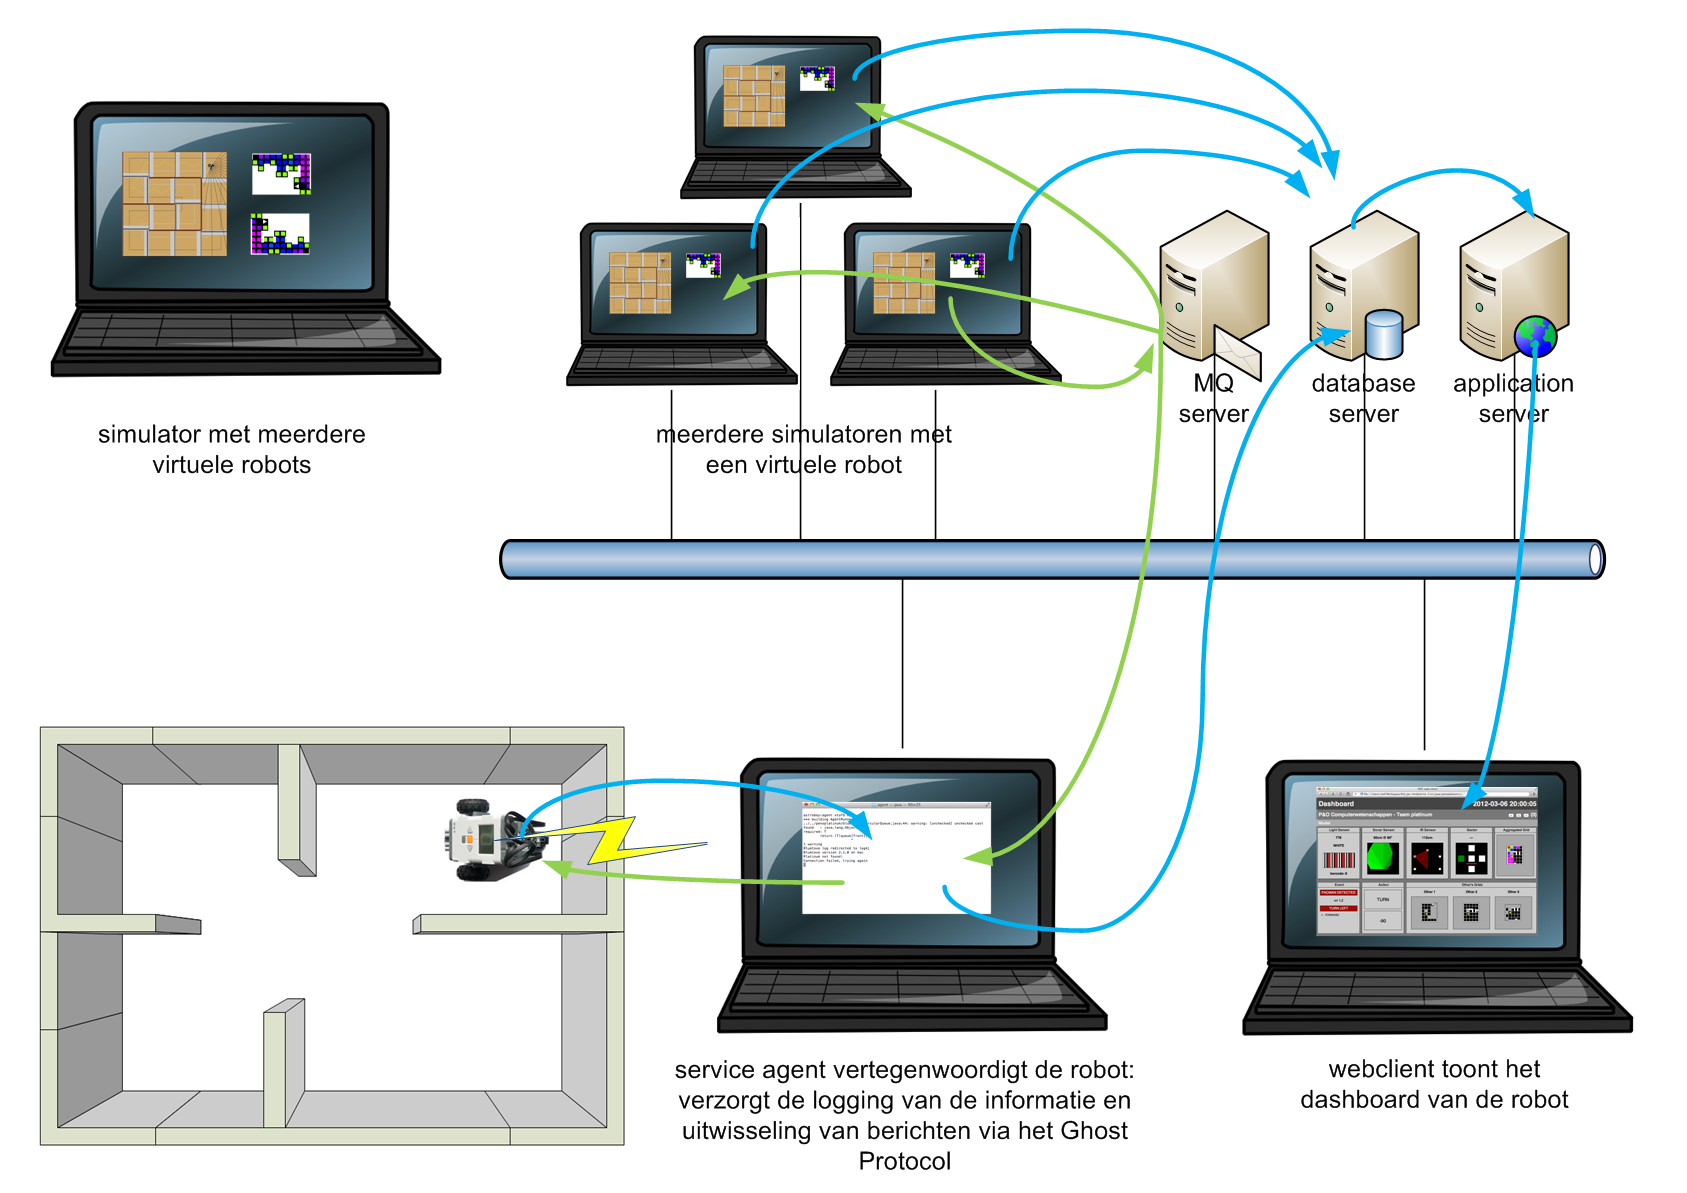
\includegraphics[width=200mm, angle=90]{resources/simulator-modi.png}
  \caption{Werking van de simulator in verschillende opstellingen.}
  \label{fig:simulator-modi}
\end{figure}

\subsection{Mini-Simulator}
\label{sect:mini-simulator}
Om het onderzoek naar het algoritme onafhankelijk te laten verlopen van de echte simulator en tevens niet te belasten met details van deze laatste, werd een mini-simulator gemaakt. Deze maakt een abstractie van de wereld en kent alleen een resolutie op niveau van sectoren zoals dit het geval is in de simulator. Figuur \ref{fig:mini-simulator} toont de mini-simulator in actie met vier gesimuleerde robots, elk vertrokken op een andere positie en met een andere ori\"entatie.

\begin{figure}[htbp]
  \centering
  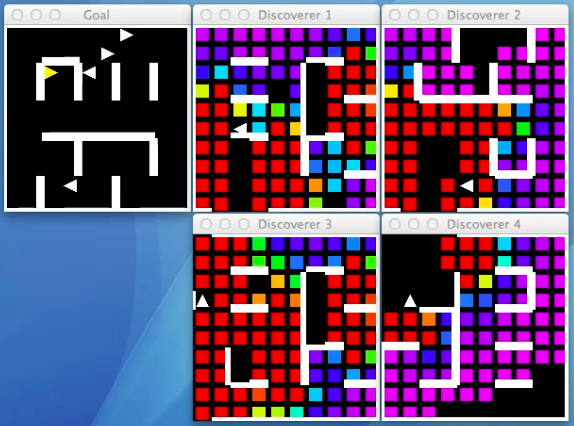
\includegraphics[width=120mm]{resources/mini-simulator.png}
  \caption{Mini-simulator in actie}
  \label{fig:mini-simulator}
\end{figure}

Door de introductie van de \emph{Driver} naast de \emph{Navigator} is er een duidelijke opdeling tussen het effectieve rijden van sector naar sector en de keuze van de volgende sector waarheen gereden moet worden. Deze abstractie is doorgetrokken in de mini-simulator die zich louter met het \emph{Navigator} niveau bezighoudt, waar de (volledige) simulator ook het niveau van de \emph{Driver} in beschouwing neemt.

Zo wordt de mini-simulator ook gebruikt om onderzoek te doen naar het geheugengebruik, nodig om al de navigator-informatie bij te houden. Net zoals bij de (volledige) simulator, is het ook mogelijk om zonder visualisatie te werken, waardoor veel scenario's kunnen getest worden.

\section{Demo 2}

De huidige simulator is zeer geschikt om visuele simulaties uit te voeren met de robot. We willen nu echter ook unit testen uitvoeren. Hiervoor hebben we besloten om visuele representatie optioneel te maken. Dit zorgt ervoor dat we in deze eenvoudigere modus niet langer gebonden zijn aan de ingebouwde vertragingen, die impliciet verbonden zijn met de visualisatie.
Dit stelt ons in staat om snel uitgebreide tests uit voeren en data te verzamelen voor analyse.
Deze functionaliteit zit al gedeeltelijk in onze simulator. De enige functionaliteit die we moeten toevoegen zijn functies om onze gesimuleerde robots te ondervragen, zoals hun positie, richting en sensorwaarden.

Overigens werden andere doelstellingen voor demo 2 met betrekking tot de simulator reeds gehaald. De simulator werkte immers al op een continu niveau en ook onzekerheden waren reeds ge\"implementeerd.

\section{Demo 3}

Functioneel werden tijdens de voorbereiding van deze demo geen aanpassingen gedaan aan de simulator. Wel werd hij, net zoals alle belangrijke componenten, onderworpen aan een grondige opkuisactie en werd de logica ingebed in een set van unit tests.

\section{Simulatie versus realiteit}

De simulator is gebouwd volgens een principe van continu\"iteit. Zo worden alle aspecten berekend volgens de fysische grootheden uit de realiteit. Alle sensoren zijn virtueel ge\"mplementeerd en berekenen op basis van de fysische eigenschappen van de echte robot de juiste verschillen tussen twee opeenvolgende stappen. Zo worden bijvoorbeeld de motoren gesimuleerd volgens het juist aantal rotaties per seconde, wat een effect heeft op de afstand die afgelegd is in relatie tot de echte omtrek van de wielen en de afstand tussen deze wielen.

Op deze manier gedraagt de robot in de simulator zich nagenoeg identiek aan zijn fysieke tegenhanger. In combinatie met het gebruiken van exact dezelfde software op de fysieke robot als in de simulator zorgt voor een zeer realiteitsgetrouw effect.

\chapter{Conclusies}

\section{Demo 1}

In appendix A werden de verschillende relevante beoordelingsdocumenten toegevoegd.

\subsection{Feedback}

De robot reed consistent en robuust. Zelfs wanneer de robot fouten maakte werden deze hersteld. In het begin las de lichtsensor foute waarden en reed de robot heen en weer. De introductie van het nieuwe algoritme om deze sensor automatisch te kalibreren lag hier aan de oorsprong. Na enige tijd was de kalibratie duidelijk beter en begon de robot alsnog het speelveld verder te verkennen. Hierbij viel op hoe robuust de implementatie van de Driver is.

De feedback van het didactische team was overwegend positief. Er werd duidelijk goed nagedacht over de softwarearchitectuur, zowel op niveau van robuustheid, uitbreidbaarheid als structuur. De gebruikte strategie i.v.m.\ Collaborative diffusion is goed gevonden en werkt duidelijk goed door zijn eenvoud. Het dashboard werd positief vermeld en de inhoud en opmaak van het verslag waren in lijn met de overige kwaliteit.

Naast opmerkingen over opmaak en verduidelijking, waren er ook tips met zicht op verbetering van de presentatie en het rijgedrag van de robot.

Als directe antwoord op deze opmerkingen kozen we voor het implementeren van een configuratie-klasse om de opstartsnelheid te verhogen, ook het presenteren zelf wordt vanaf nu beter voorbereid. Het rijgedrag wordt vooral geoptimaliseerd door het verwijderen van redundantie.

\subsection{Reflectie}

Hoewel we allemaal zeer tevreden waren met de prestatie die we leverden op de demo, zijn we nog niet tevreden over het niveau dat we willen bereiken met dit project.

We beslisten daarom om een week uit te trekken om een code review te doen. Op basis van de resultaten van die review beslissen we vervolgens wie wat zal doen en hoe grotere delen zullen aangepakt worden. Hieruit volgt dan een planning die de doelstellingen voor de overige demo's definieert. Meer uitleg over dit proces is te vinden in hoofdstuk \ref{ch:process}.

In het algemeen hebben we beslist om te blijven bij een volledig autonome robot, hoewel dit beperkingen inhoudt ten gevolge van het beperkte geheugen van de robot. Naast een doorgedreven optimalisatie van het geheugengebruik, hebben we dit ook cijfermatig onderzocht en is dit een van de parameters waar we rekening mee houden tijdens de uitvoering van de logica op de robot. Sectie \ref{sect:performance} gaat dieper in om dit aspect.

De simulator werkte niet zoals verwacht. Barcodes werden niet goed gelezen en dus hebben de robots geen gemeenschappelijke barcodes gevonden. Ook verdween de Pac-Man te snel en werden de robots terug door de nog niet verkende sector waar de Pac-Man op stond aangetrokken. Zo werd de rest van het veld niet meer verkend.

\section{Demo 2}


\subsection{Feedback}

De feedback kwam deze keer van een ander team, namelijk team zilver. Het grootste deel van deze feedback kwam neer op stijlopmerkingen i.v.m.\ het verslag. Het verslag zelf werd inhoudelijk overzichtelijk en gestructureerd bevonden. Het presentatiegedeelte kreeg echter welverdiende negatieve feedback. Zowel de virtuele simulator als de fysieke simulator faalde immers in hun uitvoering.

Ook merkten zij op dat tijdens de presentatie \'e\'en van de gesimuleerde robots een fout had gemaakt bij het importeren van gegevens van een andere robot en dat wij dit niet pro-actief zelf aangekaart hadden. 

\subsection{Reflectie}

Het rijgedrag van de robot bleef consistent met de vorige demo. De nieuwe lichtsensor implementatie bleek wel beter te werken dan de vorige keer.

De virtuele simulator bleek geen rekening te houden met het gebruik van een intern assenstel dat afwijkt van het gebruikte assenstel door de andere teams. Een spijtig voorval dat zijn oorsprong vindt in onze voorsprong uit het eerste semester. Dit werd snel opgelost en getest met de andere teams. Enkele andere interpretatieverschillen met betrekking tot het protocol werden eveneens reeds weggewerkt.

De uitvoering van de strategie was duidelijk niet geslaagd, de implementatie van de grids was dan ook niet vervolledigd, bijgevolg werd de informatie van de teams nog niet correct gecombineerd.
De doelstellingen opgesteld na demo 1 werden dus niet gehaald en daarom is het ook logisch dat de demo sterk tegenviel. We slaagden er wel in om het geheugengebruik te reduceren tot een werkbaar niveau, zonder functionaliteit te verwijderen.

\section{Demo 3}

Dit deel wordt later toegevoegd.

\chapter{Procesbeschrijving}
\label{ch:process}

\section{Demo 1}

Onze werkwijze tijdens het eerste semester heeft zijn vruchten afgeworpen. We willen deze aanpak ook in het tweede semester verder zetten. Zo volgen we opnieuw twee paden naar ons doel: enerzijds wordt er verder gewerkt aan de simulator en wordt de robot verder verbeterd. Anderzijds starten we ook een traject op dat zich focust op het einddoel.

Omdat de scope van de eerste demo in essentie zo sterkt aanleunt bij het uiteindelijke doel en omdat we met de ontwikkeling van de simulator tijdens het eerste semester een voorsprong hebben t.o.v.\ de overige teams willen we de scope van de finale demo reeds als doelstelling nemen voor de eerste demo.

Dit gaat hand in hand met de tijd die we ter beschikking hebben tijdens de eerste weken van het semester, wanneer oefenzittingen voor andere vakken nog niet begonnen zijn. We kiezen dus voor een \emph{blitzkrieg} waarbij we trachten om de totale scope in een korte tijd te realiseren, waarna we tijdens de resterende weken dan verder kunnen verfijnen.

De taken van co\"ordinator (Michiel) en secretaris (Christophe) werden opnieuw verdeeld. Ruben is de nieuwe co\"ordinator. Voor de rol van secretaris werd niet \'e\'en teamlid aangesteld, maar werd besloten om dit een gedeelde verantwoordelijkheid te maken.

Ten gevolge van overlappingen in het uurrooster en in samenspraak met het didactische team, zal Christophe gedurende twee van de vijf uren die standaard ingepland staan op maandag het team niet vervoegen. Deze uren worden enerzijds vlak voor, alsook 's avonds na deze vaste uren gepresteerd.

\section{Demo 2}

Aangezien we tijdens de demo 1 voorbereiding ons vooral gefocust hebben op de functionele scope, gebruiken we de tijd voor demo 2 om verfijning aan ons model en onze code aan te brengen. Hierbij denken we vooral aan bugfixes, het opkuisen van de code tree en het opkuisen van de klassen zelf.

Om te weten aan wat en hoe we extra aandacht moeten geven aan onze architectuur en code, evenals om iedereen in detail vertrouwd te maken met alle code, besloten we om in de eerste week na demo 1 tijd te nemen om alle code te overlopen. Tijdens dit proces hielden we een gedeeld Google docs bestand bij waarin we opmerkingen, fouten en/of vragen m.b.t.\ de code konden plaatsen. Hierop konden alle groepsleden commentaar geven of verduidelijkingen toevoegen. Deze lijst werd als basis gebruikt om dan het werk te verdelen over de groepsleden.

Naast deze aanpak gaan we ook proberen om het concept \emph{pair programming} toe te passen. Zo is het de bedoeling dat we met twee paren en \'e\'en losse speler die overal bijspringt werken. Dit gebeurt zowel tijdens als naast de zittingen op maandag.

\section{Demo 3}

Na de grote teleurstelling in demo 2 beslisten we onze aandacht op de architectuur en de code vol te houden. Onze refactoring aanpak werd wel aangevuld met het cre\"eren van een uitgebreid unit test suite. Waarbij op het moment van schrijven een dekking van meer dan zestig procent van de totale codebase is bereikt. Een dekking van honderd percent is enerzijds niet realistisch, maar is tevens ook niet nodig. Logischerwijze wensen we een dekking voor de relevante klassen. Bij de creatie van deze suite werd in parallel alle code nagekeken. Zo werd er veel ongebruikte code verwijderd en losten we een heel reeks bugs op. Aangezien we reeds tijdens de voorbereiding van de eerste demo getracht hadden de volledige scope te bereiken, waren we nu tevens in staat om functioneel alles tot in dewe  details uit werken zonder onbekende delen.

Zo werd o.a.\ de volledige interne voorstelling van de sectoren aangepakt. Met de ervaring die we opgedaan hadden tijdens de voorbereiding van demo 2, waren we nu in staat om deze implementatie sterk te verbeteren met het oog op geheugengebruik en inzetbaarheid.

Verder valt er nog op te merken dat we bij dit proces eerst bepaalde interfaces opnieuw gedefineerd hebben, zodat we allen konden werken aan afgeronde gehelen. Dit gaf natuurlijk het nadeel dat de volledige source code onbruikbaar was tot al deze gehelen opnieuw ge\"integreerd waren. We geloven er sterk in dat dit proces onze code veel stabieler heeft gemaakt en onze robot hier dus baat bij heeft.

\section{Unit testen}
\label{unittesten}

Na de eerste demo van het tweede semester werden we geconfronteerd met de gevolgen van het negeren van \'e\'en van de belangrijkste geboden van software ontwikkeling: \emph{Gij zult uw code testbaar maken en testen.} Bijna elke aanpassing aan \'e\'en deel van de code zorgde voor verschrikkelijke gevolgen aan een ander deel. Elke kleinste wijziging brak andere delen van de oplossing.

Gegeven de manier waarop de software ontwikkeld was tot dan toe, was dit niet geheel onbegrijpelijk. We hadden twee opties: verder gaan op de manier die we gehanteerd hadden en elk probleempje proberen te \emph{fixen} of structureel een ingrijpende verandering doorvoeren in de manier waarop we met de code omgingen.

Aangezien \'e\'en van de doelen van P\&O Computerwetenschappen net is om te leren in praktijk hoe een middelgroot softwareproject dient uitgebaat te worden, hebben we deze kans aangegrepen om een stap verder te gaan en zelf aan den lijve te ondervinden of en hoe een andere aanpak effectief meer stabiliteit kan brengen. We begonnen met het invoeren van structurele unit testen voor zoveel mogelijk code.

Aangezien de functionaliteit compleet was, konden we de volledige scope overzien. De architectuur die we gekozen hadden bleek een goed antwoord voor de meeste van de uitdagingen die in de opdracht vervat zaten. Vertrekkende van deze twee pijlers konden we dus sequentieel door de volledige code gaan en elke klasse op zich perfect vormgeven en voorzien van testen.

Met een codebase van ongeveer 17.000 lijnen code is dit echter geen sinecure en ging dit veel tijd vragen. Het alternatief was nog veel onzekerder: verder gaan met een onstabiele codebase zou mogelijk een onbetrouwbare oplossing met zich meebrengen en de wetenschap hieromtrent zou net een falen zijn in \'e\'en van de belangrijkste aspecten van de opdracht.

Met nog vier weken voor de finale deadline begonnen we aan een grote onderneming. Week na week groeide het volume aan testen en begon de \emph{coverage} stilaan nuttige vormen aan te nemen. Toen uitspraken als \emph{God zij dank dat we de unit testen hebben.} bij alle teamleden begonnen te rijzen, wisten we dat we op de goede weg zaten. Figuur \ref{fig:sloc} toont de evolutie van de volledige codebase en het aantal lijnen code (SLOC). Hier is duidelijk te zien dat vanaf begin april er een sterke en gestage toename is van het aantal lijnen code te wijten aan het structureel invoeren van unit testen. Ook toont deze grafiek zeer duidelijk dat ook de groei van de functionele code gestopt is en dat er zelfs een lichte daling is op te tekenen.

\begin{figure}[htbp]
  \centering
  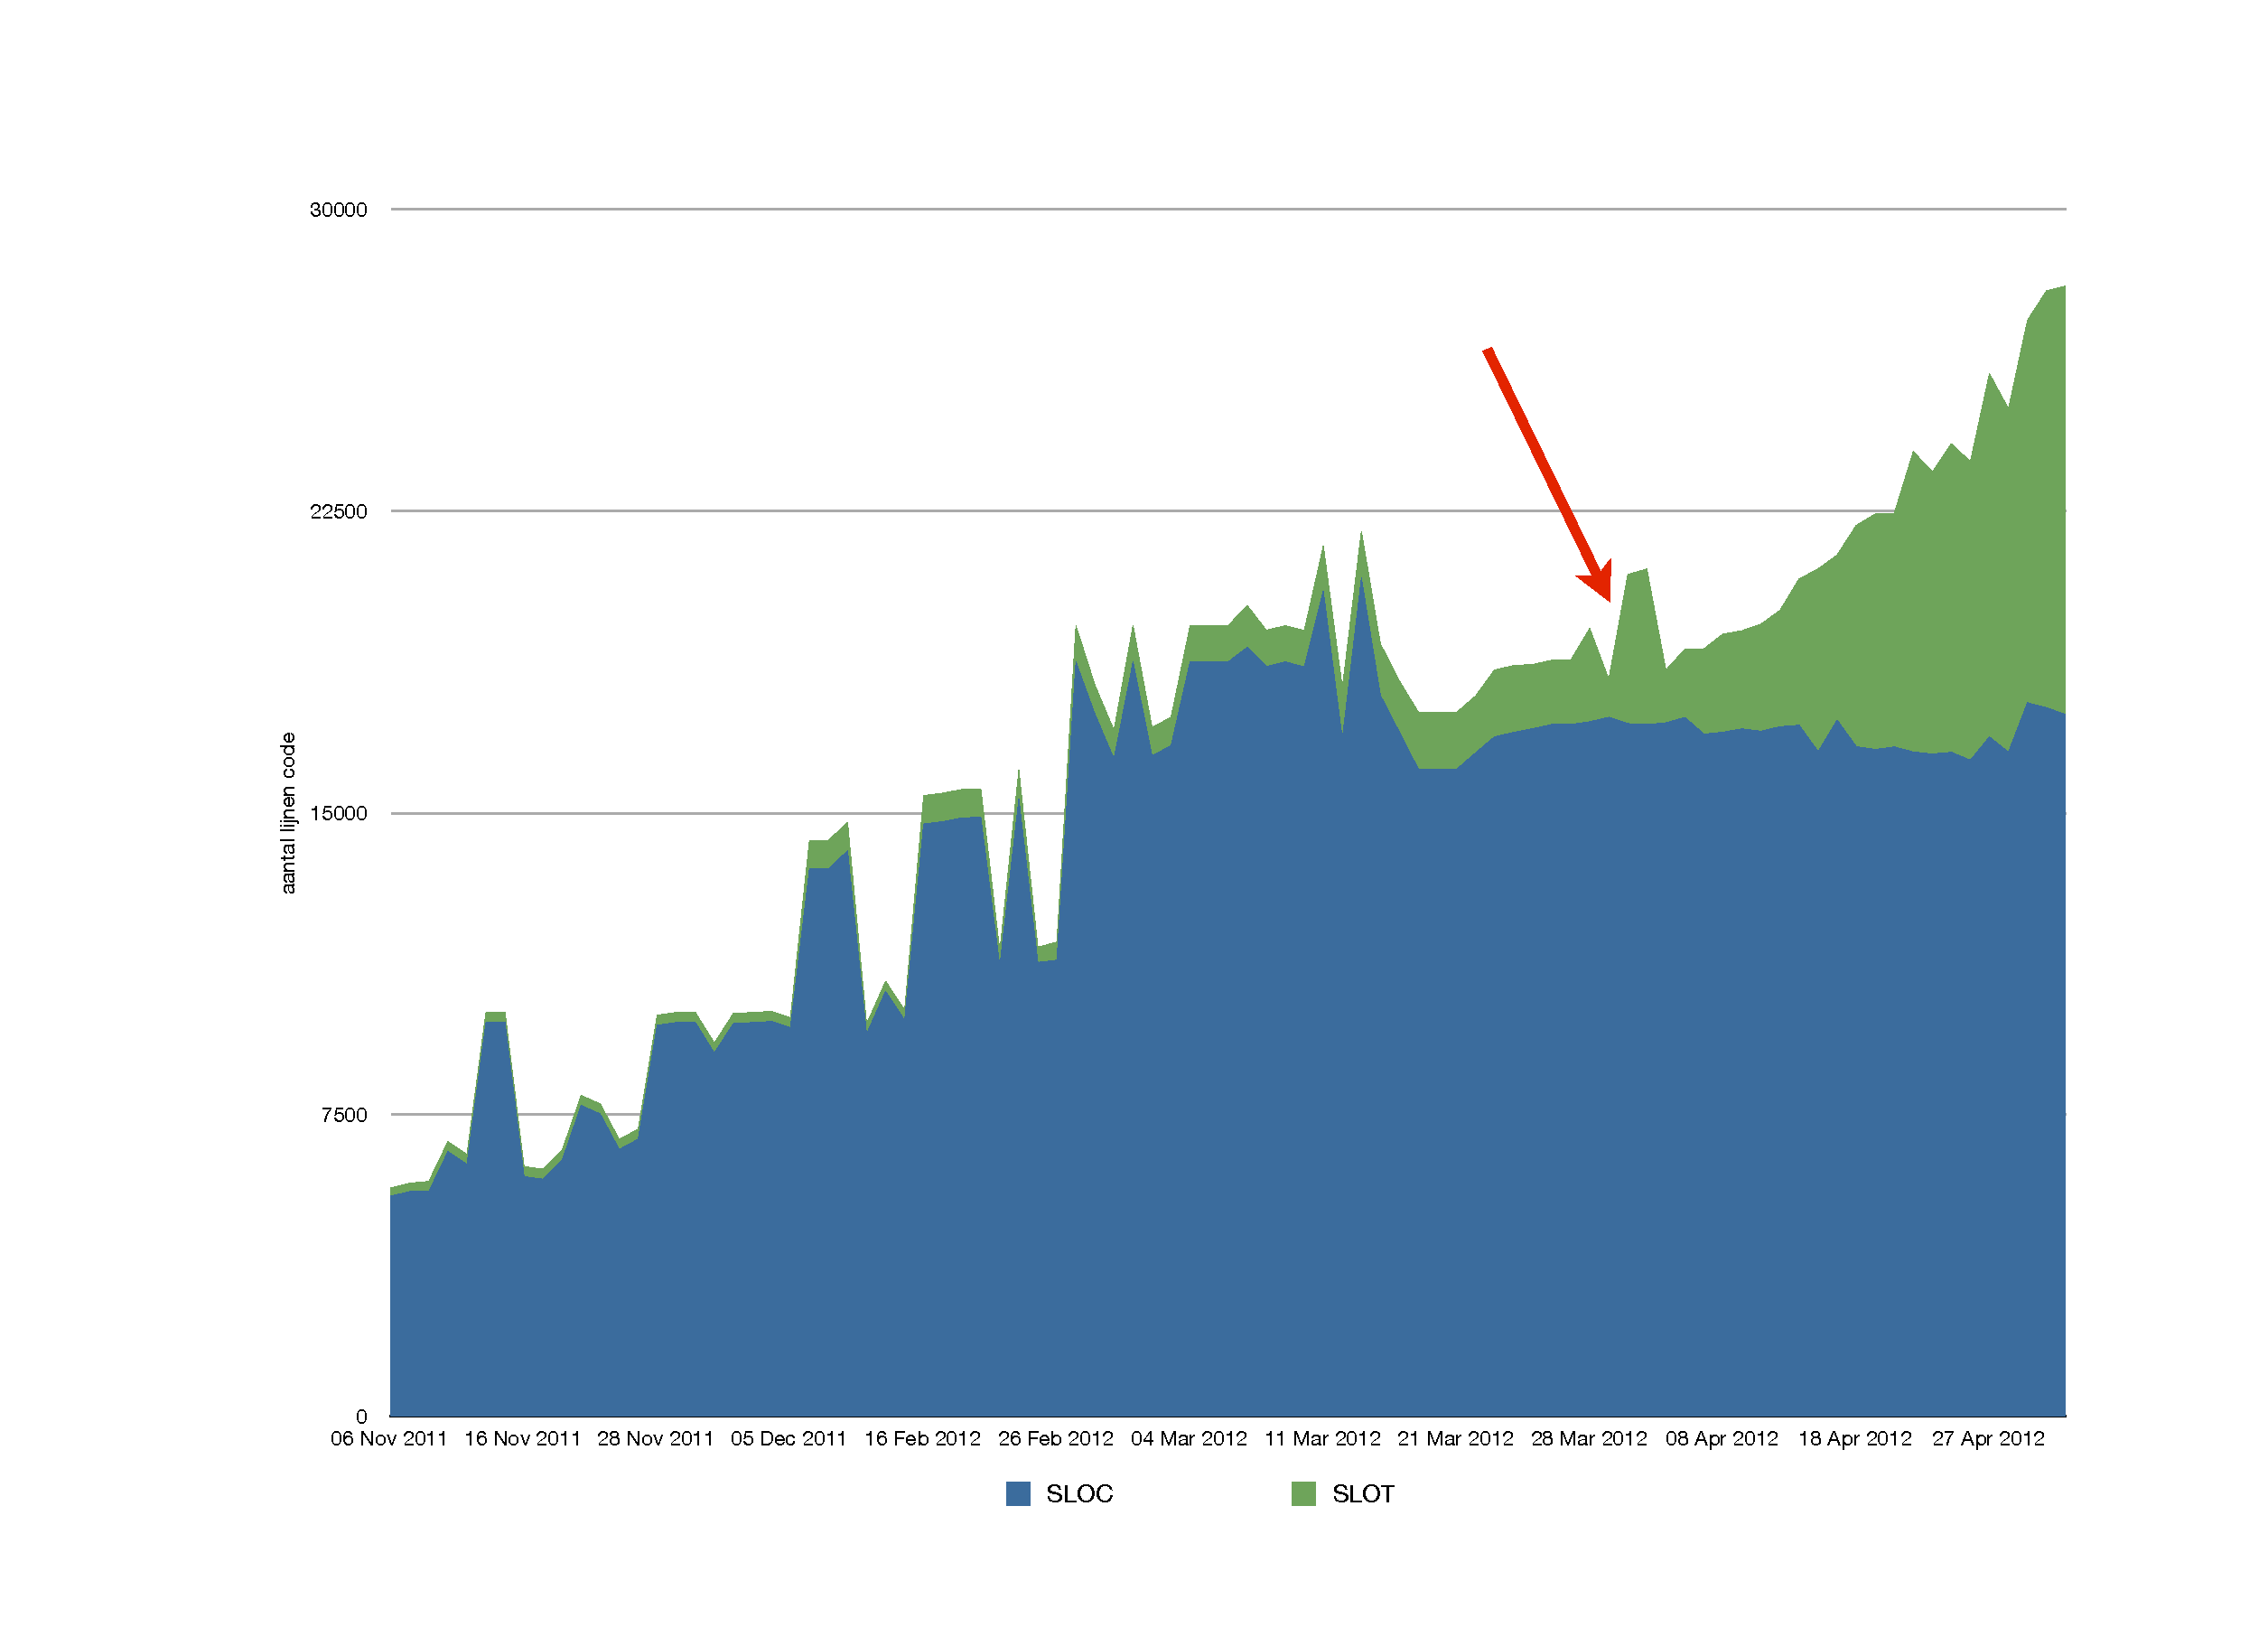
\includegraphics[width=125mm]{resources/sloc.pdf}
  \caption{Evolutie van het totale aantal SLOC en het aandeel van de unit testen}
  \label{fig:sloc}
\end{figure}

Figuur \ref{fig:coverage} toont dan weer het aantal klassen in het project samen met de \emph{coverage} van de unit test klassen. De evolutie is natuurlijk gelijklopend, maar beide grafieken bieden een ander inzicht in de evolutie. Op amper vier weken bereikten we reeds een \emph{class coverage} van meer dan 60\%.

\begin{figure}[htbp]
  \centering
  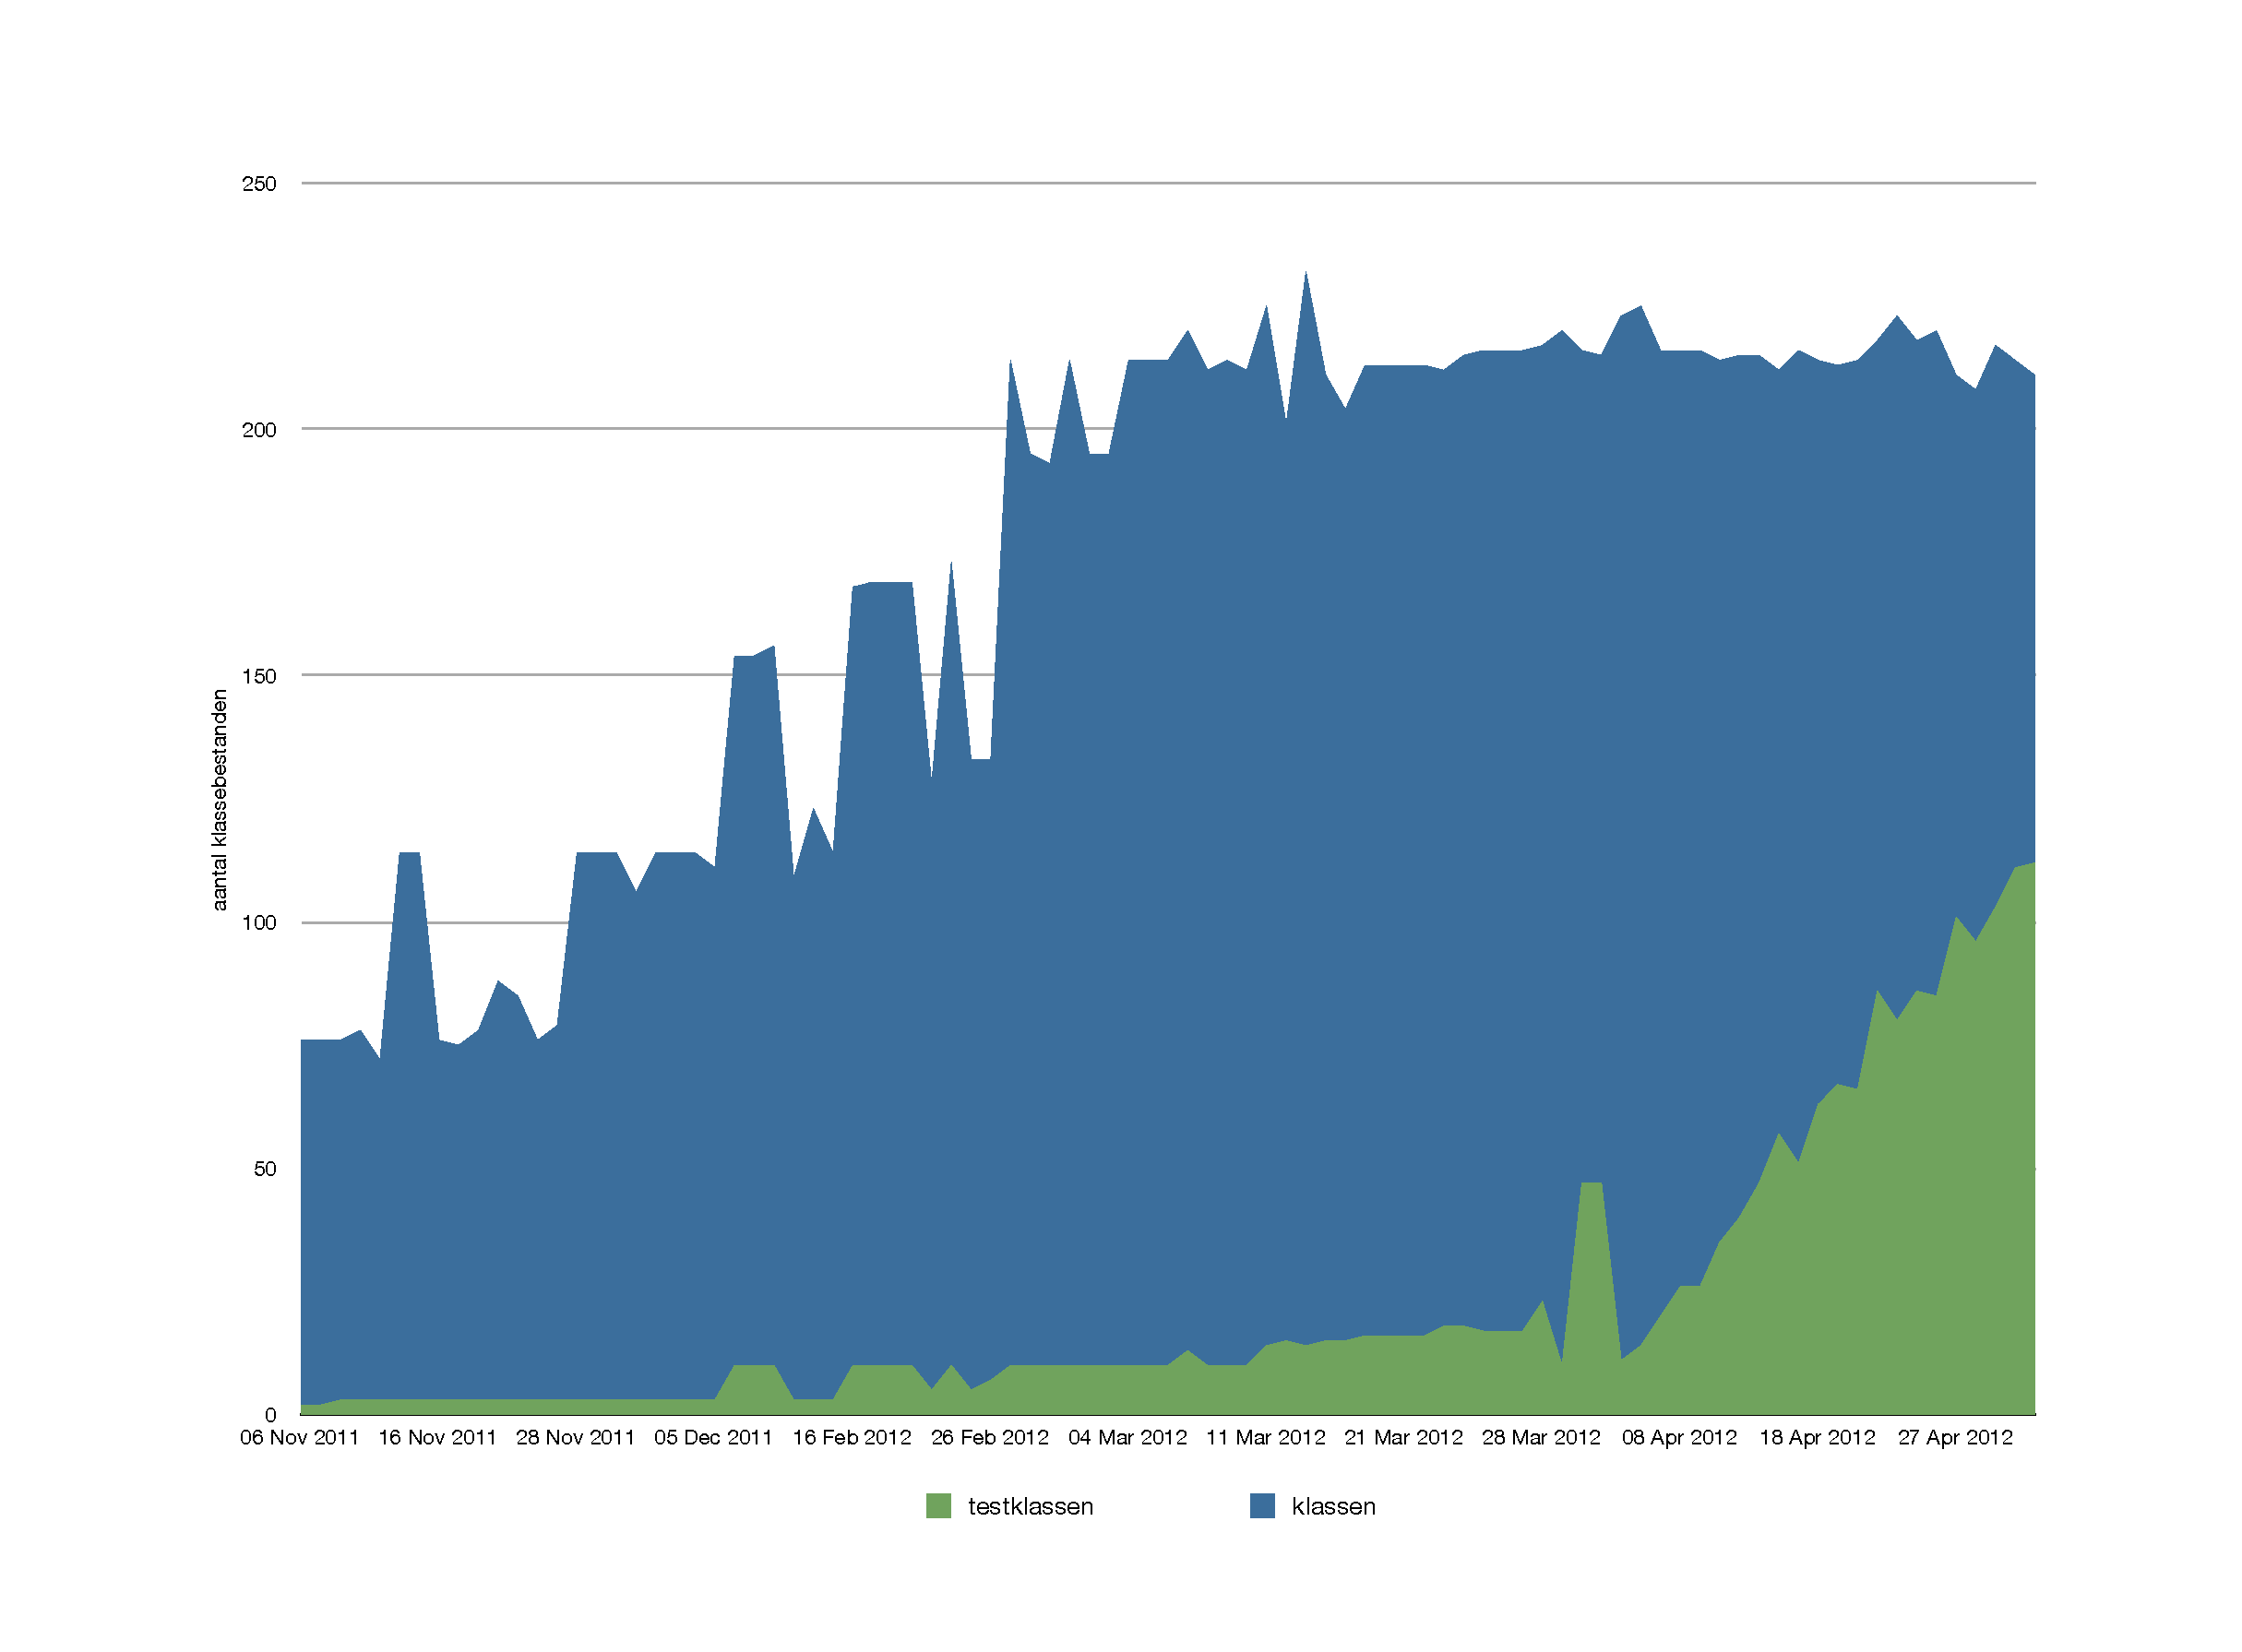
\includegraphics[width=120mm]{resources/coverage.pdf}
  \caption{Evolutie van het aantal klassen en de coverage van de unit test klassen}
  \label{fig:coverage}
\end{figure}

Alle voordelen van een codebase met een goede \emph{coverage} begonnen zich op te werpen: bij elke commit kon een \emph{RunAllTests} test suite doorlopen worden en bracht een succesvolle uitvoering een gegronde zekerheid dat een aanpassing geen problemen had teweeggebracht in andere delen van de oplossing. Figuur \ref{fig:runalltests} toont deze uitvoer en bevestiging.

\begin{figure}[htbp]
  \centering
  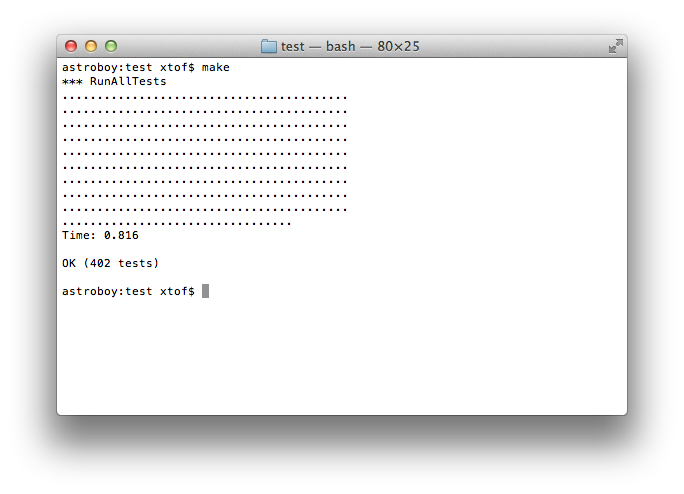
\includegraphics[width=100mm]{resources/runalltests.png}
  \caption{De RunAllTests test suite in actie.}
  \label{fig:runalltests}
\end{figure}

Deze aanpak heeft natuurlijk \'e\'en groot nadeel. Sequentieel door de volledige codebase lopen, alle code opschonen en elke klasse op zich van de nodige unit testen te voorzien, betekent dat de codebase als een geheel niet langer functioneel is. Dit was een risico dat we moesten nemen om zelf te kunnen ondervinden of deze piste inderdaad een onderbouwde zekerheid kan bieden.

Dit deel wordt nog verder aangevuld nadat de effectieve resultaten van deze onderneming bereikt zijn.

\chapter{Werkverdeling}

Dit deel wordt later toegevoegd.

\chapter{Kritische analyse}

%(a) Maak een analyse van de sterke en zwakke punten van het project. Welke punten zijn
%vatbaar voor verbetering. Wat zou je, met je huidige kennis, anders aangepakt hebben?

Dit deel wordt later toegevoegd.

\appendix

\chapter{Beoordelingen}

\section{Demo 1}
\begin{center}
Team Platinum
\end{center}

\subsection{ Verslag} 
     
     \subsubsection{1.a Grote problemen}

\begin{itemize}
	\item   in sectie 1: 
	''iedereen is ondertussen vertrouwd geraakt met de volledige architectuur''

 gevaarlijke opmerking 
\end{itemize}

   \subsubsection{1.b Kleinere opmerkingen}

 
\begin{itemize}
 \item Figuur 5.1, 5.2 dienen beter uitgelegd te zijn. Wat is wat? Legende van kleuren ontbreekt. 
 \item Figuur 4.1: fit een lijn door de punten om de bewering van exponenti\"ele lijn te ondersteunen 
 \item Referentie naar een wetenschappelijk paper kan beter in Referenties sectie (via bibtex).
 \item Sectie 4.1.1: wat is het nut van laatste zin? (wat als de robot rijdt??)
 \item Referenties naar Wikipedia zijn niet nodig, indien nodig beter verwijzen naar een boek
 \item mini simulator? welk doel heeft dit? is het niet gewoon een weergave van een simulatie?
\end{itemize}

   \subsubsection{1.c stilistische opmerkingen}

\begin{itemize}
	\item typo's: ivm $\rightarrow$ i.v.m., jlasse $\rightarrow$ klasse
\end{itemize}

\subsection{Presentatie}

	\subsubsection{2.a Presentatie zelf}
\begin{itemize}
 \item presentatie was niet voorbereid, langzame start
 \item wel een van de betere demo's
 \item denk nog eens na over optimaliseren van rijgedrag (robuustheid versus snelheid)
\end{itemize}

     \subsubsection{2.b antwoorden op vragen}
\begin{itemize}
	\item     Geen.
 
\end{itemize}
\subsection{ Positieve punten}

\begin{itemize}
 \item software zit goed in elkaar
 \item zeer aangename compacte schrijfstijl
 \item analyse van ghost protocol is zeer goed
 \item Collaborative diffusion is knap gevonden
 \item dashboard gui is duidelijk
\end{itemize}

\section{Demo 2}
\begin{center}
Team Platinum
\end{center}

\subsection{ Verslag} 
     
     \subsubsection{1.a Grote problemen}

\begin{itemize}
	\item    Opgelegde structuur niet nageleefd: strategie en softwareontwerp omgewisseld;
 beoordelingen in appendix A in plaats van in conclusie.
\item Sectie 6: Sequentiediagramma toevoegen van bijvoorbeeld sensorwaardeaanroep. Hoe snel wordt er bemonsterd?
\end{itemize}

   \subsubsection{1.b Kleinere opmerkingen}

 
\begin{itemize}
 \item Namen van de teamleden niet vermeld op voorblad.
 \item Sectie 2.1: De ghosts, meer bepaald de gesimuleerde robots, hebben w\'el kennis van het parcours nodig (volledige
kaart gegeven voor elke demo), weliswaar niet rechtstreeks. Nuancering hierover nodig in het verslag.
 \item Sectie 4.1.1: Op welke manier kan de robot gemakkelijker bestuurd worden door de NXT Brick om te keren?
 \item Sectie 4.1.1: Foto's van de robot kunnen helpen de beschrijving te ondersteunen.
 \item Sectie 6: Is er overwogen om gebruik te maken van een PC i.p.v.\ de robot alles te laten bijhouden en zelf te
laten beslissen? Hierdoor zou immers het geheugenprobleem verhoplen kunnen worden.
 \item Sectie 6.1.4: Waarom is een minimum van 60 FPS noodzakelijk? Na ongeveer 17 ms (=1000/60) zijn (waar-
schijnlijk) nog niet alle gemeten waarden van de sensoren veranderd. Is dit bijgevolg niet redundant?
\item Sectie 6.1.4, deel geheugengebruik: `mini-simulator': er wordt verwezen naar een verdere sectie in het verslag;
dit is ongebruikelijk.
\item Meermaals vermeld dat er in het eerste semester reeds een simulator gemaakt is (samenvatting, sectie 7 pag. 26
en 27).
\end{itemize}

   \subsubsection{1.c stilistische opmerkingen}

\begin{itemize}
	\item Subjectief taalgebruik, onder meer:
	\begin{itemize}
	\item ''Spijtig genoeg...'', pag. 6;
	\item ''... zou het dom zijn te veronderstellen dat...'', pag. 12.
	\end{itemize}
	\item Inconsistentie, onder meer:
\begin{itemize}
	\item Pac-Man, de Pac-Man, Pac-Man-robot;
	\item robot, ghost, spook;
	\item IR, infrarood (en samenstellingen).
\end{itemize}
	\item Schrijf-/taal-/tikfouten:
	
\begin{itemize}
	\item Samenvatting: jaaroverschrijdend $\rightarrow$ jaaroverschrijdend, Pac-Man-spel$\rightarrow$ Pac-Manspel, Open Bron project $\rightarrow$ Open Sourceproject;
	\item Sectie 2.1: ''staat (...) stil op het parcours'': in $\rightarrow$ op;
	\item Sectie 2.3.2: Pac-Man spel $\rightarrow$ Pac-Manspel;
	\item Sectie 3.2: ''(...) en bespreken we de voor- en nadelen ervan''; mbt. $\rightarrow$ m.b.t.;
	\item Sectie 4.1.2: ''(\ldots) IR-bal en -sensor.''$\rightarrow$  '' (\ldots) IR-bal en -sensor.'', AC modus ! AC-modus (ook van
toepassing op analoge situaties);
	\item Sectie 6.1.1: Leesteken vergeten na laatste zin;
	\item Sectie 6.1.2: configuratie aanpassingen $\rightarrow$ configuratieaanpassingen;
	\item Sectie 6.1.3: muur-informatie $\rightarrow$ muurinformatie;
	\item Sectie 7.1.3: Simulator Modi $\rightarrow$ Simulatormodi, MQ-server $\rightarrow$ MQ-server;
	\item Sectie 9.2: Laatste `zin' van deze sectie heeft geen werkwoord;
	\item Sectie 10: team lid $\rightarrow$ teamlid.
\end{itemize}
	\item Vreemd taalgebruik:
  \begin{itemize}
	\item Samenvatting: programmatie, ''effectieve fysieke robot'';
	\item \textit{Map} veelvuldig gebruikt i.p.v.\ \textit{kaart}, o.m. op pag. 3.
\end{itemize}
	\item Andere opmerkingen:
\begin{itemize}
	\item bij voorkeur enkele aanhalingstekens gebruiken i.p.v.\ dubbele, in het bijzonder bij het benadrukken van \'e\'en
woord; nog beter is gebruik maken van cursivering i.p.v.\ aanhalingstekens, dit is minder storend bij het
lezen;
	\item zo weinig mogelijk woorden benadrukken om leesbaarheid te bevorderen, bv. sectie 5.1: ''In de voorstelling ontstaat er een ''deuk'' in de ''geur'' achter de ''ghost''.'';
	\item veel passieve zinnen (wordt, worden, werden,...);
	\item gebruik van het woord \textit{men} bij voorkeur te vermijden;
	\item \LaTeX afkortingen zoals i.v.m.\ en t.o.v.\ laten eindigen met backslash, zodat een 'normale' spatie gebruikt
wordt i.p.v.\ een grotere zoals op het einde van een zin gebruikelijk is;
	\item bij voorkeur gebruik maken van \textit{sections} i.p.v.\ chapter in de \LaTeX-broncode; hoofdstukken zijn eerder gebruikelijk bij boeken en cursussen.
\end{itemize}
\end{itemize}

\subsection{Presentatie}

	\subsubsection{2.a Presentatie zelf}
\begin{itemize}
 \item Paar minuten demostratietijd verloren door te laat aanwezig op demo. Hierdoor is bijvoorbeeld niet gedemonstreerd of de fysieke robot Pac-Man kan signaleren en/of insluiten.
 \item Niet zelf gezegd op de demo dat de kaarten foutief zijn samengevoegd.
\end{itemize}

     \subsubsection{2.b antwoorden op vragen}
\begin{itemize}
	\item    Geen duidelijk antwoord op de vraag waarom de kaarten verkeerd toegevoegd zijn.
 
\end{itemize}
\subsection{ Positieve punten}

\begin{itemize}
 \item Algemene indruk van het verslag is positief:
 
\begin{itemize}
	\item vlotte schrijfstijl, hoewel soms informeel en indruisend tegen de regels van een wetenschappelijk verslag;
	\item sectie 6.1.4 in het bijzonder is erg goed geschreven: aangenaam om te lezen en wetenschappelijk onderbouwd.
\end{itemize}
 \item Algemene indruk van de presentatie is positief:
\begin{itemize}
	\item de presentatie was kort en bondig, hoofdzaken kwamen aan bod, details zijn achterwege gelaten;
	\item correct taalgebruik tijdens de presentatie.
\end{itemize}
\end{itemize}

\section{Demo 2: Beoordeling Team Rood}
\begin{center}
Team Rood
\end{center}

\subsection{ Verslag} 
     
\paragraph{Vorige Beoordeling toegepast?}

Algemeen gezien is er nog steeds een grote overlap tussen de verschillende hoofdstukken en houdt men zich niet goed aan de onderverdeling.
\par Voetnoten zouden een verbetering zijn, want deze verbergen details en kunnnen bijvoorbeeld verwijzen naar een verder hoofstuk als iets nog moet uitgelegd worden (bvb \textit{NearestIncompleteSectorFinder}). Dit geldt niet enkel voor voetnoten, maar ook in het algemeen. Men zou minder moeten herhalen in het verslag en ook moeten vermelden als er iets verder in de tekst wordt uitgelegd.
\subsubsection{1.a Grote problemen}

\begin{itemize}
	\item Waarom wordt er geen geaggregeerde voorstelling van de info gemaakt i.p.v.\ de info te negeren? Een voorstelling van de huidige wereld met behulp van info komende van alle robots zou logischer zijn, er is immers geen geheugengebrek. Mogelijks is dit voor later gehouden.
	\item Waarom wordt alles op de PC gedaan? Misschien kan men informatie toevoegen i.v.m.\ onderzoek naar de bluetoothverbinding? Alles stond in het eerste semester op de robot dus dient er toch uitgelegd te worden waarom men deze overschakeling doet?
	\item Er werd volgens ons te weinig aandacht besteed aan het protocol. Wat waren de voor- en nadelen op het vlak van implementatie voor team rood? Wat hadden ze achteraf gezien anders gedaan, wat hebben ze niet nodig, wat willen ze er nog aan toevoegen, etc ?
\end{itemize}

   \subsubsection{1.b Kleinere opmerkingen}

 
\begin{itemize}
	\item sectie 2.1.1: De boodschappen worden in plain text verstuurd en zijn ook begrijpbaar voor mensen, wat debugging en implementatie eenvoudiger maakt.(Dit maakt implementatie net minder eenvoudig)
	\item sectie 2.1.2: \ldots bijzonder sterk is, kan Pac-Man door de muren gezien worden.(men bedoelt waarschijnlijk dat er reflecties zijn, slecht verwoord)
	\item sectie 2.2.2:\ldots er geen botsingen tussen de ghosts\ldots(wel botsingen?)
	\item sectie 4.1.3: De eerste sector van dit pad wordt uitgestuurd naar de robot via DataSender.(de robot krijgt enkel richtingen toegestuurd?)
	\item sectie 4.1.4: \ldots de binnenkomende informatie genegeerd.(Is dit enkel na mergen? Waarom zelfs niet daarna iets doen met deze info? Als meerdere remotes dezelfde info bevestigen, wordt deze toch geloofwaardig.)
		\item sectie 4.2.3: Waarom staat de BarcodeScanner op de robot en niet op de computer? Dit is toch logica. Wordt de bluetoothcommunicatie dan overbelast met lichtsensor waarden? 
	\item sectie 5.1.2: Een alternatieve, na\"ieve\ldots(Dit is een overbodige zin.)
\end{itemize}

   \subsubsection{1.c stilistische opmerkingen}


\begin{itemize}
	\item sectie 1.1  : Belangrijk is dat\ldots (zinsconstructie)
	\item sectie 2.1.1: zodra i.p.v van zodra (meermaals in tekst), beide i.p.v beiden,
	\item sectie 3.1.2: (hardware) is een overbodige vermelding  
	\item sectie 3.2.2: veel voorkomend (veelvoorkomend)
	\item sectie 4.1.1: geupdateted (ge\"updatet), data is een meervoud
	\item sectie 4.1.3: receiver- en sendervelden (streepje en velden aan sender, vaak geen streepjes)
	\item sectie 4.2.2: de zien is  (  te zien is ), achtereenvolgens( s i.p.v d)
	\item sectie 4.4.1: Er zijn enkele enkele(dubbel)
	\item sectie 5.1.2: Dit om te vermijden dat (i.p.v.\ dit om in de te vermijden \ldots)
	\item sectie 5.2.1: Een stuk doolhof dat niet verkend kan worden(\ldots)wordt niet verkend. overbodig(meermaals overbodige constructies)
	\item sectie 6.1.2: dat de robot(tweemaal achtereen)
	\item sectie 7.1.1: een keer in de mist gegaan(de mist ingegaan)
	\item sectie 8.1  : Er was geen tijd om te testen \ldots (in deze zin missen enkele leestekens)
	\item overige     : overbodige komma's ; zinnen zonder werkwoord (bvb sectie 3.1.2: zoals bijvoorbeeld het wit\ldots); samenstellingen schrijven met spatie ertussen is fout; tussen persoonsvormen komma gebruiken;  soms enkelvoud gebruikt i.p.v.\ meervoud bij werkwoorden; foutief gebruik van koppeltekens bij samenstellingen
	\item consistentie: IRSeeker en IR-Seeker; cursiveren van de klassenamen, methoden,enz. ; RabbitMQ-protocol; Integerwaarde(aan elkaar soms af elkaar)
\end{itemize}

\subsection{Presentatie}

	\subsubsection{2.a Presentatie zelf}
\begin{itemize}
	\item De inleiding was niet zo spontaan als gewenst, er werd van een papier afgelezen.
	\item Er werd benadrukt dat de correcties op het rijden waren verwijderd om de snelheid op te hogen, dit kwam de robuustheid van de robot duidelijk niet ten goede aangezien er drie maal manueel gecorrigeerd moest worden. Nochtans werd er op voorhand vermeldt dat aan het rijgedrag van de robot hard gewerkt is.
	\item sectie 4.2.2: Het is de verantwoordelijkheid van de computer om ervoor te zorgen dat de robot niet tegen een muur rijdt. Lagen hier de fouten misschien aan, zijn er tests over de vertraging van de communicatie?
\end{itemize}
     \subsubsection{2.b antwoorden op vragen}
\subsection{ Positieve punten}
\begin{itemize}
	\item Robot redesign werd zeer goed onderbouwd.
	\item De scenario analyses zijn zeer goed voor de strategie, gevaar is natuurlijk wel dat als dit te veel gedaan wordt dat het verslag zijn bondigheid uit het oog verliest. Deze scenario's kunnen ook de indruk wekken dat er enkel gedachtenexperimenten werden opgezet omtrent zeer specifieke situaties, i.p.v.\ de algemene strategie uitgebreid te testen. Het blijft wel een zeer aangename manier om de denkstrategie toe te lichten.
\end{itemize}
 
\chapter{Grafische User Interface}

Het project voorziet verschillende gebruikers interfaces: Zo is er een dashboard dat informatie geeft over verschillende parameters van de werking van een robot. Daarnaast geeft een simulator een beeld van de gesimuleerde wereld en van de manier waarop de gesimuleerde robot de wereld ervaart. Tot slot is er een administratie \emph{shell} om een robot van op afstand commando's door te sturen.

\section{Dashboard}

Het \emph{Dashboard} is een web toepassing die informatie ontvangt uit de databank waarin de \emph{Gateway} de ontvangen feedback van een robot opslaat. De web toepassing ontvangt deze informatie via een \emph{JSONP}\footnote{JSONP wordt typisch opgebouwd met een lang-lopende connectie waarover de server constant nieuwe Javascript commando's verstuurd. Deze worden op de client uitgevoerd, waardoor updates van bijvoorbeeld data kunnen verwerkt worden. Zie ook \url{http://en.wikipedia.org/wiki/JSONP}} connectie. Op deze manier kan de web toepassing toch in real-time een informatiestroom van de robot ontvangen.

Figuur \ref{fig:dashboard_overview} toont het \emph{Dashboard} met al zijn samenstellende delen. Het principe van het \emph{Dashboard} bestaat uit een reeks van onafhankelijke panelen die elk een conceptueel deel van de informatie waarover de robot beschikt voorstellen. Zo zijn er typisch panelen voor elk van de sensoren. Een paneel voor een sensor toont enerzijds de laatst gelezen waarde, maar tracht ook een nuttige histogram van de informatie aan te bieden. Zo is er bijvoorbeeld voor de lichtsensor een voortschrijdende balk waarop barcodes visueel ook kunnen herkend worden. De sonar wordt weergegeven zoals een klassieke sonar, enz. Daarnaast worden de verschillende \emph{Grids} gevisualiseerd. Tot slot zijn er nog panelen die informatie geven over de gebeurtenissen waarop de robot reageert en de acties dat hij hierdoor onderneemt.

Dankzij de uitwerking aan de hand van HTML en Javascript kunnen we het \emph{Dashboard} zeer eenvoudig aanpassen en panelen bijmaken of verwijderen.

\begin{figure}[htbp]
  \centering
  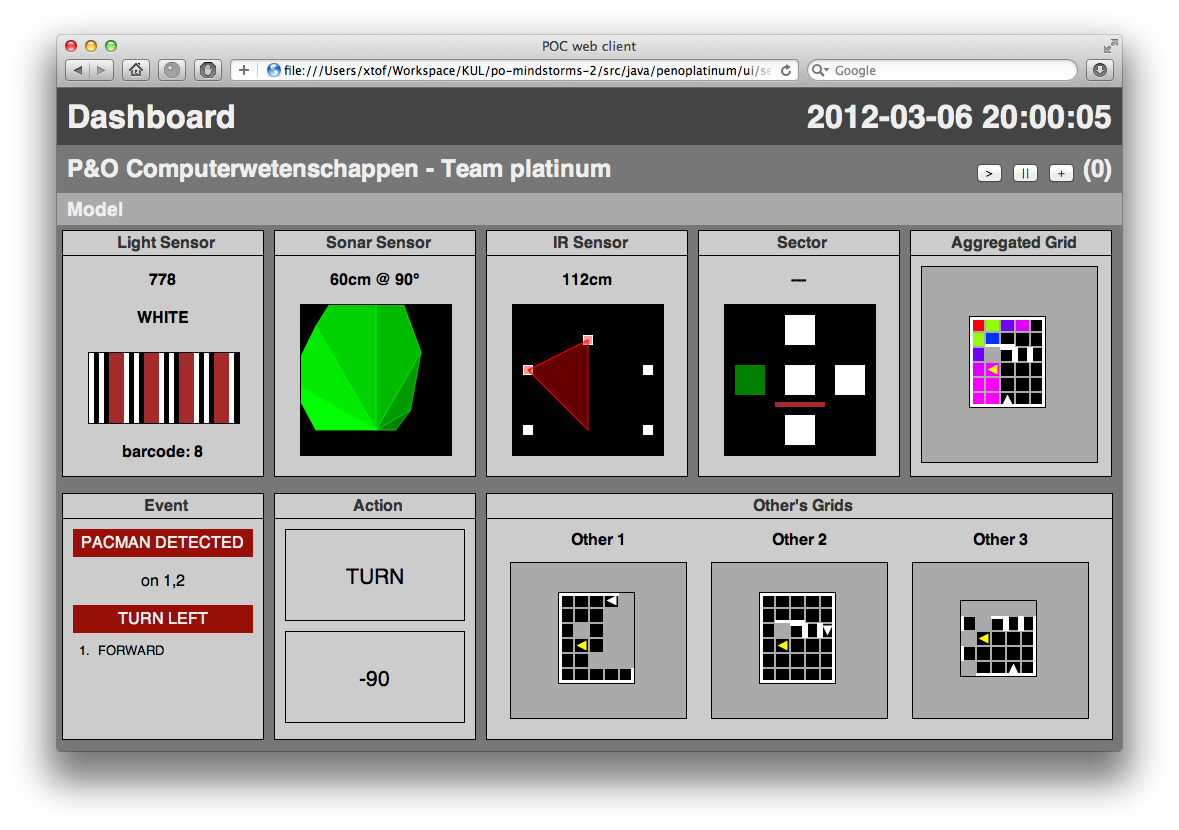
\includegraphics[width=150mm]{resources/dashboard.png}
  \caption{Overzicht van de functionaliteit van het Dashboard}
  \label{fig:dashboard_overview}
\end{figure}

\section{Simulator}

De simulator, weergegeven in figuur \ref{fig:simulator2}, bestaat uit twee grote delen: \'e\'en overzichtsscherm en maximaal vier kleinere deelschermen voor de visualisatie van de \emph{Grid} van elk van de gesimuleerde robots. Deze visualisatie van de \emph{Grid} wordt voorzien door de \emph{GridView}, een optionele component die verbonden kan worden met de effectieve \emph{Grid} van een robot.

\begin{figure}[htbp]
  \centering
  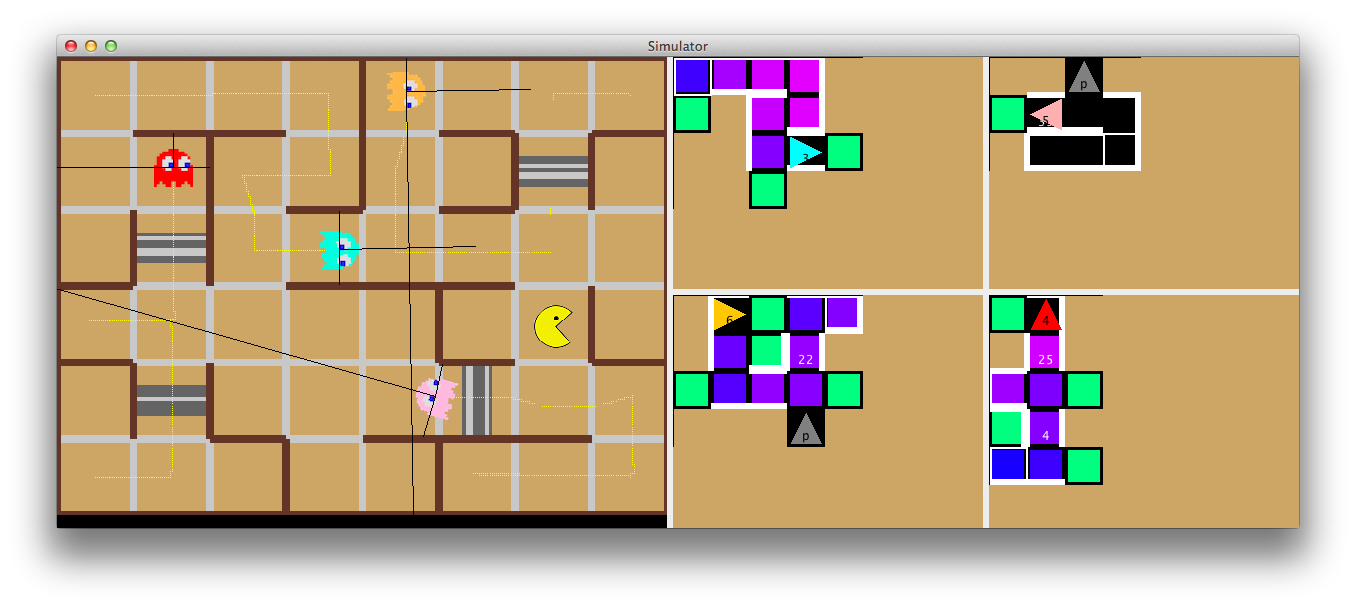
\includegraphics[width=150mm]{resources/simulator2.png}
  \caption{De Simulator simuleert vier robots.}
  \label{fig:simulator2}
\end{figure}

De simulator wordt opgestart aan de hand van de \emph{SimulationRunner}. Deze applicatie biedt tal van mogelijkheden om de simulator op te starten. Zo kan elke mogelijke \emph{Driver}, \emph{Navigator}, ... opgegeven worden op de command line, waardoor het een uiterst flexibele tool wordt. Figuur \ref{fig:simulationrunner} toont het help scherm met alle opties.

\begin{figure}[htbp]
  \centering
  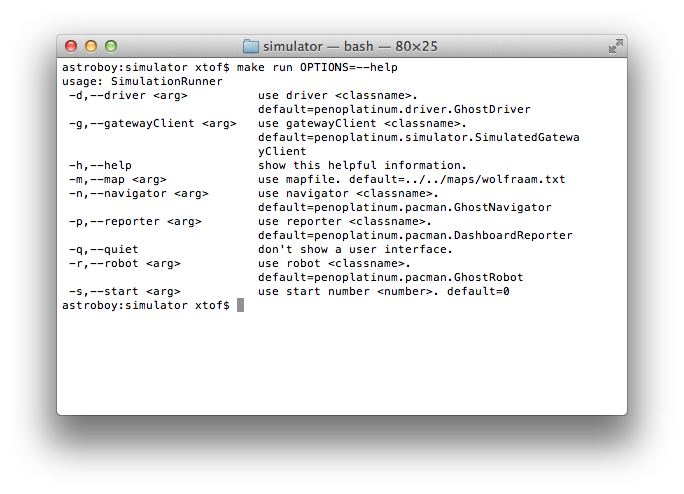
\includegraphics[width=110mm]{resources/simulationrunner.png}
  \caption{Opties om de simulator op te starten.}
  \label{fig:simulationrunner}
\end{figure}

\section{RASH - Robot Administratie Shell}

De \emph{Robot Administratie Shell}, kortweg \emph{rash}, werd in het leven geroepen om commando's door te sturen naar de robot. De nood voor een dergelijke tool ontstond uit de noodzaak om bijvoorbeeld een robot te verplichten om het gewone verloop van de start-procedure, zoals gedefinieerd in het \emph{GhostProtocol}, te doorbreken en de robot te verplichten om toch te starten.

Aangezien er in het protocol impliciet ruimte is gelaten om eigen commando's te specificeren, door het verplichten van het negeren van onbekende commando's, en deze via de message queue te sturen, kozen we om een generiek eigen \emph{custom} commando te gebruiken:

\begin{center}
{\tt <name> PENOPLATINUM\_CMD <signature> <counter> <command>}
\end{center}

Hierin is \emph{name} de naam van onze robot, \emph{signature} een MD5 hash die dient om het \emph{PENOPLATINUM\_CMD} te beveiligen, \emph{counter} een teller om te zorgen dat elk bericht uniek is en niet meerdere malen zou geaccepteerd worden en \emph{command} een commando met eventueel eigen argumenten. Door deze opbouw is het makkelijk om meer eigen commando's toe te voegen. Voorlopig is een \emph{FORCESTART} commando op deze manier ge\"implementeerd. Figuur \ref{fig:rash_help} toont \emph{rash} opgestart met het \emph{help} argument, waardoor een overzicht wordt getoond van de mogelijke command line argumenten. 

\begin{figure}[htbp]
  \centering
  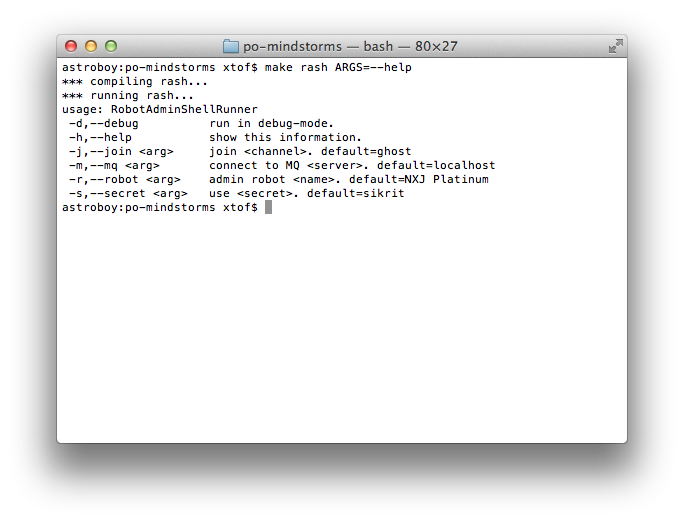
\includegraphics[width=110mm]{resources/rash_help.png}
  \caption{Het help overzicht van rash.}
  \label{fig:rash_help}
\end{figure}

Figuur \ref{fig:rash_forcestart} toont \emph{rash} in actie\footnote{\emph{rash} voorziet een \emph{debug} mode waarbij de boodschappen die naar de MQ server wordt verstuurd op de console getoond worden.}, waarbij het \emph{FORCESTART} commando uitgevoerd wordt.

\begin{figure}[htbp]
  \centering
  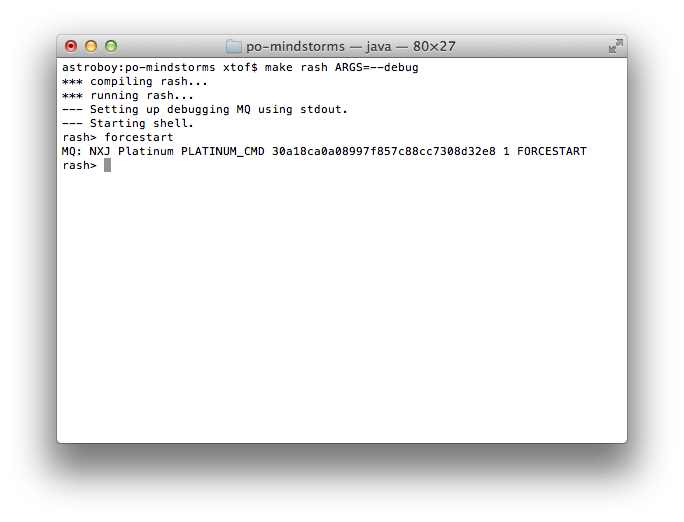
\includegraphics[width=110mm]{resources/rash_forcestart.png}
  \caption{Het versturen van het FORCESTART commando met rash.}
  \label{fig:rash_forcestart}
\end{figure}

De opstelling met \emph{rash} bood ons nog een bijkomende opportuniteit. Zo kunnen we \emph{rash} ook gebruiken om een log van een sessie opnieuw af te spelen. Dit maakt het mogelijk om een reeks commando's van andere robots te simuleren en zo een uitgebreide communicatie tussen andere robots en onze eigen robot te testen zonder effectief andere robots nodig te hebben.

\begin{figure}[htbp]
  \centering
  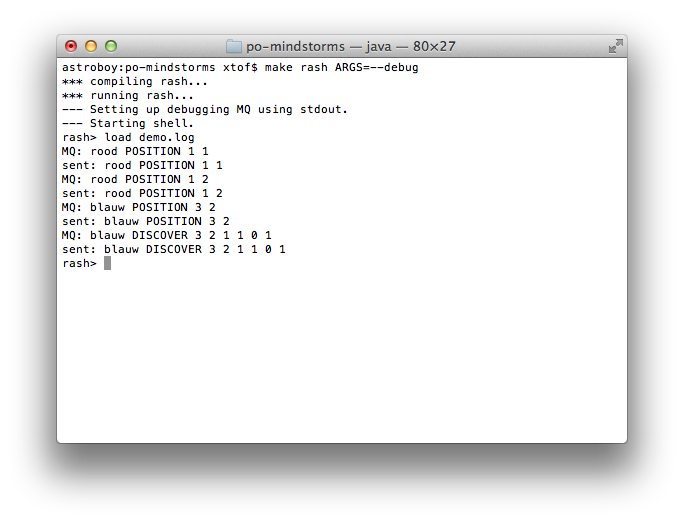
\includegraphics[width=110mm]{resources/rash_load.png}
  \caption{Met behulp van rash kan een log van commando's verstuurd worden.}
  \label{fig:rash_load}
\end{figure}

De keuze om van \emph{rash} een aparte applicatie te maken was evident: het beheren van de robot op dit niveau is niet verenigbaar met het eenvoudig volgen van informatie omtrent de robot, zoals dit in het \emph{Dashboard} mogelijk is. De gevoeligheid van de functionaliteit is veel hoger. Anderzijds is het moeten toepassen van deze acties eerder uitzonderlijk. Toch is het design van \emph{rash} zo uitgewerkt dat een integratie met bijvoorbeeld het \emph{Dashboard} mogelijk is. De effectieve logica is ondergebracht in een \emph{RobotAdminClient}. Deze is ingebed in de eigenlijke gebruikersinterface, de \emph{RobotAdminShell}. Mits het toevoegen van een schrijfbaar veld in het \emph{Dashboard} en het opvangen van de inhoud van dit veld in de \emph{Gateway}, kan deze laatste de \emph{RobotAdminClient} zonder aanpassingen gebruiken om ook langs dit kanaal ook dezelfde functionaliteit te implementeren.

\chapter{Klasse Diagrammen}

Dit deel wordt later toegevoegd.

\chapter{Planning}

\label{appendix:planning}

\begin{longtable}{|l|l|l|l|l|l|l|l|l|}
\caption{Overzicht tijdsbesteding} \\
\hline \\[-2ex]
  \multicolumn{1}{l}{week } & 
  \multicolumn{1}{l}{Michiel} &
  \multicolumn{1}{l}{Florian} &
  \multicolumn{1}{l}{Ruben} &
  \multicolumn{1}{l}{Thomas}&
  \multicolumn{1}{l}{Christophe}&
  \multicolumn{1}{l}{Totaal}&
  \multicolumn{1}{l}{AVG}&
  \multicolumn{1}{l}{Lopend AVG}
  \\[0.5ex] \hline \\[-1.8ex]
\endfirsthead
\hline
avg & 20,0 & 18,0 & 18,1 & 17,9 & 21,3 &  & 19,06 &  \\ 
\hline
sum & 260 & 234 & 235 & 233 & 277 & 1239 &  &  \\ 
\hline
1 & 12 & 9 & 13 & 14 & 16,5 & 64,5 & 12,90 & 12,90 \\ 
\hline
2 & 16,5 & 14 & 14 & 15 & 17,5 & 77 & 15,40 & 14,15 \\ 
\hline
3 & 32,5 & 15 & 21 & 17 & 29 & 114,5 & 22,90 & 17,07 \\ 
\hline
4 & 49 & 24 & 33 & 28 & 32 & 166 & 33,20 & 21,10 \\ 
\hline
5 & 8 & 9 & 11 & 18 & 14 & 60 & 12,00 & 19,28 \\ 
\hline
6 & 26 & 23 & 24 & 36 & 36 & 145 & 29,00 & 20,90 \\ 
\hline
7 & 14 & 8 & 5 & 5 & 20 & 52 & 10,40 & 19,40 \\ 
\hline
8 & 3 & 0 & 0 & 0 & 13 & 16 & 3,20 & 17,38 \\ 
\hline
9 & 0 & 0 & 0 & 0 & 11 & 11 & 2,20 & 15,69 \\ 
\hline
10 & 11 & 24 & 18 & 22 & 2 & 77 & 15,40 & 15,66 \\ 
\hline
11 & 19 & 31 & 19 & 28 & 22 & 119 & 23,80 & 16,40 \\ 
\hline
12 & 50 & 55 & 53 & 38 & 41 & 237 & 47,40 & 18,98 \\ 
\hline
13 & 19 & 22 & 24 & 12 & 23 & 100 & 20,00 & 19,06 \\ 
\hline
\end{longtable}\normalsize

% Table generated by Excel2LaTeX from sheet 'Log'
% Table generated by Excel2LaTeX from sheet 'Sheet1'
\begin{landscape}
\begin{longtable}{llp{7cm}p{10cm}l}
\caption{Michiel tijdsbesteding} \\

\hline \hline \\[-2ex]
  \multicolumn{1}{l}{Dag} & \multicolumn{1}{l}{Datum} &
  \multicolumn{1}{p{7cm}}{omschrijving team} &
  \multicolumn{1}{p{10cm}}{omschrijving Michiel} &
  \multicolumn{1}{l}{Uren}  \\[0.5ex] \hline \\[-1.8ex]
\endfirsthead

\multicolumn{5}{l}{{\tablename} \thetable{} -- Continued} \\[0.5ex]
\hline \hline \\[-2ex]
  \multicolumn{1}{l}{Dag} & \multicolumn{1}{l}{Datum} &
  \multicolumn{1}{p{7cm}}{omschrijving team} &
  \multicolumn{1}{p{10cm}}{omschrijving Michiel} &
  \multicolumn{1}{l}{Uren}  \\[0.5ex] \hline \\[-1.8ex]
\endhead

\multicolumn{5}{l}{{Continued on Next Page\ldots}} \\
\endfoot

\\[-1.8ex] \hline \hline
\endlastfoot

\hline
 &  &  &  & 260 \\ 
\hline
Mon & 13-feb.-2012 & P\&O sessie,discussie aanpak, research pacman ed,  & commissie & 5 \\ 
\hline
Wed & 15-feb.-2012 &  &  & 5 \\ 
\hline
Fri & 17-feb.-2012 &  &  & 2 \\ 
\hline
Mon & 20-feb.-2012 & P\&O sessie & Testen IR,commissie & 5 \\ 
\hline
Tue & 21-feb.-2012 &  &  & 2 \\ 
\hline
Wed & 22-feb.-2012 & Testen IR & Testen IR & 7,5 \\ 
\hline
Fri & 24-feb.-2012 & Driving/map voor bouw robot &  &  \\ 
\hline
Sat & 25-feb.-2012 & Simulator+behaviour &  & 2 \\ 
\hline
Mon & 27-feb.-2012 & P\&O sessie &  & 8 \\ 
\hline
Tue & 28-feb.-2012 & verslag &  & 8,5 \\ 
\hline
Wed & 29-feb.-2012 &  &  & 7 \\ 
\hline
Thu & 1-mrt.-2012 &  & onderzoek naar mogelijke verbeteringen op gebied van rondrijden & 7 \\ 
\hline
Fri & 2-mrt.-2012 &  &  & 2 \\ 
\hline
Sat & 3-mrt.-2012 & code bekeken voor verslag &  &  \\ 
\hline
Sun & 4-mrt.-2012 & verslag &  &  \\ 
\hline
Mon & 5-mrt.-2012 & P\&O sessie & commissie, code integration mini-simulator and real simulator & 5 \\ 
\hline
Tue & 6-mrt.-2012 & verslag, debugging & lichtsensor herimplementatie & 8 \\ 
\hline
Wed & 7-mrt.-2012 &  & verslag, ghost protocol & 9 \\ 
\hline
Thu & 8-mrt.-2012 &  & Testen ghost protocol, implementatie RobotBluetoothAgent, schrijven scanner implementatie, aanpassen code voor lejos, schrijven ontbrekende code in lejos & 9 \\ 
\hline
Fri & 9-mrt.-2012 & Memory Management & Optimalisatie robot, bespreking memory management, implementatie barcodes in protocol, implementatie grid importing & 5 \\ 
\hline
Sun & 11-mrt.-2012 &  & refactored unit tests, fixed all build errors, work on grid importing, barcode bugfixing, MQ bugfixing, Dashboard agent implementation & 13 \\ 
\hline
Mon & 12-mrt.-2012 & P\&O Sessie & Barcode bugfixing, grid mapping bugfixing, pacman protocl implementatie, reverse mapping implementatie, dashboardagent implementatie & 7 \\ 
\hline
Sat & 17-mrt.-2012 &  &  & 1 \\ 
\hline
Mon & 19-mrt.-2012 & P\&O Sessie, overlopen resultaten code review en taakverdeling & Vergadering + planning, scheidsrechtercommisie, initial model refactoring & 5 \\ 
\hline
Tue & 20-mrt.-2012 &  & completed model refactoring, merged minisimulator robot implementation with the actual robot implementation, cleanup of robot project & 4 \\ 
\hline
Wed & 21-mrt.-2012 & Inleveren verslag 2 & Added light consistency test, fixed barcode bug, adding barcodes to swinggridview & 3 \\ 
\hline
Thu & 22-mrt.-2012 &  & Added barcodes to the minisimulator & 1 \\ 
\hline
Sat & 24-mrt.-2012 &  & implementatie gridmerging & 6 \\ 
\hline
Sun & 25-mrt.-2012 &  & implementatie gridmerging & 7 \\ 
\hline
Mon & 26-mrt.-2012 & P\&O Sessie / Demo 2 &  & 5 \\ 
\hline
Sat & 31-mrt.-2012 &  & Unit testen voor grid package & 6 \\ 
\hline
Sun & 1-apr.-2012 &  & Transformatietesten grid & 3 \\ 
\hline
Mon & 2-apr.-2012 & Paasvakantie & Sector interface & 3 \\ 
\hline
Mon & 16-apr.-2012 & P\&O Sessie &  & 5 \\ 
\hline
Sun & 22-apr.-2012 &  & Mergen branches + fixen various tests, Implementatie LinkedSector + testen & 6 \\ 
\hline
Mon & 23-apr.-2012 & P\&O Sessie & Interface grid + implementatie, compilation errors in test fixen & 5 \\ 
\hline
Tue & 24-apr.-2012 &  & Implementatie Linkedgrid & 2 \\ 
\hline
Wed & 25-apr.-2012 &  & Testen Linkedgrid & 4 \\ 
\hline
Sun & 29-apr.-2012 &  & Implemented Aggregatedgrid + sector, transformedgrid + sector, MultiGhostGrid. Partially tested transformedgrid & 8 \\ 
\hline
Mon & 30-apr.-2012 & P\&O Sessie & Fixed all transformedgrid and transformedsector issues + tested. Implemented aggregatedsector test, work on aggregatedgrid test & 8 \\ 
\hline
Tue & 1/mei/12 &  & Grid optimalisatie & 8 \\ 
\hline
Wed & 2/mei/12 & Inleveren verslag 3 & Grid optimalisatie & 8 \\ 
\hline
Thu & 3/mei/12 &  & Grid optimalisatie & 6 \\ 
\hline
Fri & 4/mei/12 &  & Grid optimalisatie & 8 \\ 
\hline
Sun & 6/mei/12 &  & Grid optimalisatie & 12 \\ 
\hline
Mon & 7/mei/12 & Finale Demo & GRID transitief mergen + sector collapse & 15 \\ 
\hline
Wed & 9/mei/12 & Eindverslag &  & 3\\ 
\hline
Mon & 14/mei/12 & Finale Presentatie &  & 1 \\ 
\hline
\end{longtable}
\normalsize


\begin{longtable}{llp{7cm}p{10cm}l}
\caption{Florian tijdsbesteding} \\

\hline \hline \\[-2ex]
  \multicolumn{1}{l}{Dag} & \multicolumn{1}{l}{Datum} &
  \multicolumn{1}{p{7cm}}{omschrijving team} &
  \multicolumn{1}{p{10cm}}{omschrijving Florian} &
  \multicolumn{1}{l}{Uren}  \\[0.5ex] \hline \\[-1.8ex]
\endfirsthead

\multicolumn{5}{l}{{\tablename} \thetable{} -- Continued} \\[0.5ex]
\hline \hline \\[-2ex]
  \multicolumn{1}{l}{Dag} & \multicolumn{1}{l}{Datum} &
  \multicolumn{1}{p{7cm}}{omschrijving team} &
  \multicolumn{1}{p{10cm}}{omschrijving Florian} &
  \multicolumn{1}{l}{Uren}  \\[0.5ex] \hline \\[-1.8ex]
\endhead

\multicolumn{5}{l}{{Continued on Next Page\ldots}} \\
\endfoot

\\[-1.8ex] \hline \hline
\endlastfoot

\hline
 &  &  &  & 234 \\ 
\hline
Mon & 13-feb.-2012 & P\&O sessie,discussie aanpak, research pacman ed,  & simulator refactoring en nieuwe features & 4 \\ 
\hline
Wed & 15-feb.-2012 &  & Sector Opdeling & 5 \\ 
\hline
Mon & 20-feb.-2012 & P\&O sessie &  & 5 \\ 
\hline
Tue & 21-feb.-2012 &  & IR & 3 \\ 
\hline
Wed & 22-feb.-2012 & Testen IR & Testen IR & 6 \\ 
\hline
Fri & 24-feb.-2012 & Driving/map voor bouw robot &  &  \\ 
\hline
Sat & 25-feb.-2012 & Simulator+behaviour &  &  \\ 
\hline
Mon & 27-feb.-2012 & P\&O sessie &  & 5 \\ 
\hline
Tue & 28-feb.-2012 & verslag & verslag & 5 \\ 
\hline
Wed & 29-feb.-2012 &  & verslag & 5 \\ 
\hline
Thu & 1-mrt.-2012 &  & onderzoek naar mogelijke verbeteringen op gebied van rondrijden &  \\ 
\hline
Sat & 3-mrt.-2012 & code bekeken voor verslag &  &  \\ 
\hline
Sun & 4-mrt.-2012 & verslag &  &  \\ 
\hline
Mon & 5-mrt.-2012 & P\&O sessie & verslag & 5 \\ 
\hline
Tue & 6-mrt.-2012 & verslag, debugging & lichtsensor herimplementatie & 5 \\ 
\hline
Wed & 7-mrt.-2012 &  & verslag, ghost protocol & 7 \\ 
\hline
Thu & 8-mrt.-2012 &  & pair programming michiel & 5 \\ 
\hline
Fri & 9-mrt.-2012 & Memory Management &  & 2 \\ 
\hline
Mon & 12-mrt.-2012 & P\&O Sessie &  & 5 \\ 
\hline
Wed & 14-mrt.-2012 & Review code tree  & Bitwiseoperations & 4 \\ 
\hline
Mon & 19-mrt.-2012 & P\&O Sessie, overlopen resultaten code review en taakverdeling & verslag  & 5 \\ 
\hline
Wed & 21-mrt.-2012 & Inleveren verslag 2 &  & 2 \\ 
\hline
Sat & 24-mrt.-2012 &  & verslag rood+colors +dashboardagent+collision & 9 \\ 
\hline
Sun & 25-mrt.-2012 &  & verslag +collision & 7 \\ 
\hline
Mon & 26-mrt.-2012 & P\&O Sessie / Demo 2 &  & 8 \\ 
\hline
Mon & 16-apr.-2012 & P\&O Sessie &  & 5 \\ 
\hline
Tue & 17-apr.-2012 &  & unit testen & 4 \\ 
\hline
Wed & 18-apr.-2012 &  & unit testen & 5 \\ 
\hline
Thu & 19-apr.-2012 &  & unit testen & 4 \\ 
\hline
Sat & 21-apr.-2012 &  & unit & 6 \\ 
\hline
Mon & 23-apr.-2012 & P\&O Sessie & unit & 5 \\ 
\hline
Tue & 24-apr.-2012 &  & unit & 4 \\ 
\hline
Wed & 25-apr.-2012 &  & unit & 4 \\ 
\hline
Thu & 26-apr.-2012 &  & unit & 3 \\ 
\hline
Fri & 27-apr.-2012 &  & unit & 4 \\ 
\hline
Sat & 28-apr.-2012 &  & unit & 7 \\ 
\hline
Sun & 29-apr.-2012 &  & unit & 4 \\ 
\hline
Mon & 30-apr.-2012 & P\&O Sessie & verslag & 10 \\ 
\hline
Tue & 1/mei/12 &  & grid fixes & 8 \\ 
\hline
Wed & 2/mei/12 & Inleveren verslag 3 & grid testing & 8 \\ 
\hline
Thu & 3/mei/12 &  & grid testing & 6 \\ 
\hline
Fri & 4/mei/12 &  & grid testing & 6 \\ 
\hline
Sat & 5/mei/12 &  & grid testing & 5 \\ 
\hline
Sun & 6/mei/12 &  & fixes, unit testen, etc & 12 \\ 
\hline
Mon & 7/mei/12 & Finale Demo & Memory, grid, code shrinking etc & 15 \\ 
\hline
Wed & 9/mei/12 & Eindverslag &  & 6 \\ 
\hline
Mon & 14/mei/12 & Finale Presentatie &  & 1 \\ 
\hline
\end{longtable}
\normalsize

\begin{longtable}{llp{7cm}p{10cm}l}
\caption{Ruben tijdsbesteding} \\

\hline \hline \\[-2ex]
  \multicolumn{1}{l}{Dag} & \multicolumn{1}{l}{Datum} &
  \multicolumn{1}{p{7cm}}{omschrijving team} &
  \multicolumn{1}{p{10cm}}{omschrijving Ruben} &
  \multicolumn{1}{l}{Uren}  \\[0.5ex] \hline \\[-1.8ex]
\endfirsthead

\multicolumn{5}{l}{{\tablename} \thetable{} -- Continued} \\[0.5ex]
\hline \hline \\[-2ex]
  \multicolumn{1}{l}{Dag} & \multicolumn{1}{l}{Datum} &
  \multicolumn{1}{p{7cm}}{omschrijving team} &
  \multicolumn{1}{p{10cm}}{omschrijving Ruben} &
  \multicolumn{1}{l}{Uren}  \\[0.5ex] \hline \\[-1.8ex]
\endhead

\multicolumn{5}{l}{{Continued on Next Page\ldots}} \\
\endfoot

\\[-1.8ex] \hline \hline
\endlastfoot

\hline
 &  &  &  & 235 \\ 
\hline
Mon & 13-feb.-2012 & P\&O sessie,discussie aanpak, research pacman ed,  & simulator refactoring en nieuwe features, Projectleider & 6 \\ 
\hline
Tue & 14-feb.-2012 &  &  & 2 \\ 
\hline
Wed & 15-feb.-2012 &  &  & 5 \\ 
\hline
Mon & 20-feb.-2012 & P\&O sessie & Projectleider & 5 \\ 
\hline
Tue & 21-feb.-2012 &  & IRSeeker & 4 \\ 
\hline
Wed & 22-feb.-2012 & Testen IR & Testen IR & 5 \\ 
\hline
Mon & 27-feb.-2012 & P\&O sessie & Projectleider & 6 \\ 
\hline
Tue & 28-feb.-2012 & verslag &  & 7 \\ 
\hline
Wed & 29-feb.-2012 &  &  & 3 \\ 
\hline
Thu & 1-mrt.-2012 &  & onderzoek naar mogelijke verbeteringen op gebied van rondrijden & 5 \\ 
\hline
Mon & 5-mrt.-2012 & P\&O sessie & Projectleider verslag & 5 \\ 
\hline
Tue & 6-mrt.-2012 & verslag, debugging & barcodes, verslag & 6 \\ 
\hline
Wed & 7-mrt.-2012 &  & verslag nalezen & 7 \\ 
\hline
Thu & 8-mrt.-2012 &  & MazeProtocol & 4 \\ 
\hline
Fri & 9-mrt.-2012 & Memory Management & MazeProtocol, IR in simulator, bugfixes & 3 \\ 
\hline
Sun & 11-mrt.-2012 &  &  & 8 \\ 
\hline
Mon & 12-mrt.-2012 & P\&O Sessie & Testen robot, Framerate verhogen op robot, pacman herkennen & 6 \\ 
\hline
Wed & 14-mrt.-2012 & Review code tree  &  & 5 \\ 
\hline
Mon & 19-mrt.-2012 & P\&O Sessie, overlopen resultaten code review en taakverdeling & verslag & 5 \\ 
\hline
Tue & 20-mrt.-2012 &  & verslag  refactoring & 3 \\ 
\hline
Wed & 21-mrt.-2012 & Inleveren verslag 2 & refactoring & 6 \\ 
\hline
Sat & 24-mrt.-2012 &  & barcodegedrag voor robot & 5 \\ 
\hline
Sun & 25-mrt.-2012 &  & Robot, bluetooth  memorytests & 5 \\ 
\hline
Mon & 26-mrt.-2012 & P\&O Sessie / Demo 2 &  & 5 \\ 
\hline
Mon & 16-apr.-2012 & P\&O Sessie & unit testen map & 5 \\ 
\hline
Sat & 21-apr.-2012 &  & unit testen simulator & 8 \\ 
\hline
Sun & 22-apr.-2012 &  & unit testen sensoren & 5 \\ 
\hline
Mon & 23-apr.-2012 & P\&O Sessie & unit testen sensoren & 6 \\ 
\hline
Tue & 24-apr.-2012 &  &  & 2 \\ 
\hline
Sat & 28-apr.-2012 &  &  & 6 \\ 
\hline
Sun & 29-apr.-2012 &  &  & 5 \\ 
\hline
Mon & 30-apr.-2012 & P\&O Sessie &  & 9 \\ 
\hline
Tue & 1/mei/12 &  &  & 9 \\ 
\hline
Wed & 2/mei/12 & Inleveren verslag 3 &  & 5 \\ 
\hline
Thu & 3/mei/12 &  &  & 5 \\ 
\hline
Fri & 4/mei/12 &  &  & 5 \\ 
\hline
Sat & 5/mei/12 &  &  & 8 \\ 
\hline
Sun & 6/mei/12 &  & Robot: barcodes en lijnen & 12 \\ 
\hline
Mon & 7/mei/12 & Finale Demo & Pacman, Memory issues & 15 \\ 
\hline
Tue & 8/mei/12 &  & verslag & 5 \\ 
\hline
Wed & 9/mei/12 & Eindverslag & verslag & 3 \\ 
\hline
Mon & 14/mei/12 & Finale Presentatie &  & 1 \\ 
\hline
\end{longtable}
\normalsize

\begin{longtable}{llp{7cm}p{10cm}l}
\caption{Thomas tijdsbesteding} \\

\hline \hline \\[-2ex]
  \multicolumn{1}{l}{Dag} & \multicolumn{1}{l}{Datum} &
  \multicolumn{1}{p{7cm}}{omschrijving team} &
  \multicolumn{1}{p{10cm}}{omschrijving Thomas} &
  \multicolumn{1}{l}{Uren}  \\[0.5ex] \hline \\[-1.8ex]
\endfirsthead

\multicolumn{5}{l}{{\tablename} \thetable{} -- Continued} \\[0.5ex]
\hline \hline \\[-2ex]
  \multicolumn{1}{l}{Dag} & \multicolumn{1}{l}{Datum} &
  \multicolumn{1}{p{7cm}}{omschrijving team} &
  \multicolumn{1}{p{10cm}}{omschrijving Thomas} &
  \multicolumn{1}{l}{Uren}  \\[0.5ex] \hline \\[-1.8ex]
\endhead

\multicolumn{5}{l}{{Continued on Next Page\ldots}} \\
\endfoot

\\[-1.8ex] \hline \hline
\endlastfoot
\hline
 &  &  &  & 233 \\ 
\hline
Mon & 13-feb.-2012 & P\&O sessie,discussie aanpak, research pacman ed,  & simulator refactoring en nieuwe features & 5 \\ 
\hline
Tue & 14-feb.-2012 &  &  & 3 \\ 
\hline
Wed & 15-feb.-2012 &  &  & 2 \\ 
\hline
Sat & 18-feb.-2012 &  & Sector Opdeling & 1 \\ 
\hline
Sun & 19-feb.-2012 &  & Sector Opdeling & 3 \\ 
\hline
Mon & 20-feb.-2012 & P\&O sessie & Testen IR/opkuisen code & 6 \\ 
\hline
Tue & 21-feb.-2012 &  & Research/nauwkeurigheid robot & 4 \\ 
\hline
Wed & 22-feb.-2012 & Testen IR &  & 2 \\ 
\hline
Fri & 24-feb.-2012 & Driving/map voor bouw robot &  & 1 \\ 
\hline
Sat & 25-feb.-2012 & Simulator+behaviour &  & 2 \\ 
\hline
Mon & 27-feb.-2012 & P\&O sessie & Sector & 6 \\ 
\hline
Tue & 28-feb.-2012 & verslag &  & 4 \\ 
\hline
Wed & 29-feb.-2012 &  &  & 1 \\ 
\hline
Thu & 1-mrt.-2012 &  & onderzoek naar mogelijke verbeteringen op gebied van rondrijden & 2 \\ 
\hline
Sat & 3-mrt.-2012 & code bekeken voor verslag & code bekeken voor verslag & 2 \\ 
\hline
Sun & 4-mrt.-2012 & verslag & verslag & 2 \\ 
\hline
Mon & 5-mrt.-2012 & P\&O sessie & verslag & 6 \\ 
\hline
Tue & 6-mrt.-2012 & verslag, debugging & barcodes, verslag & 5 \\ 
\hline
Wed & 7-mrt.-2012 &  & verslag, protocol,... & 8 \\ 
\hline
Thu & 8-mrt.-2012 &  &  & 3 \\ 
\hline
Fri & 9-mrt.-2012 & Memory Management & Implementatie, sensors in simulator, IR & 3 \\ 
\hline
Sun & 11-mrt.-2012 &  &  & 3 \\ 
\hline
Mon & 12-mrt.-2012 & P\&O Sessie & Testen robot, bugfixes,... & 5 \\ 
\hline
Tue & 13-mrt.-2012 &  & code review: action, bluetooth, driver,... & 3 \\ 
\hline
Wed & 14-mrt.-2012 & Review code tree  & code review: map, modelprocessors, sensors & 2 \\ 
\hline
Thu & 15-mrt.-2012 &  & code review: vizualization + start simulator & 4 \\ 
\hline
Fri & 16-mrt.-2012 &  & code review: simulator & 2 \\ 
\hline
Sat & 17-mrt.-2012 &  & code review: simulator & 2 \\ 
\hline
Mon & 19-mrt.-2012 & P\&O Sessie, overlopen resultaten code review en taakverdeling & verslag & 5 \\ 
\hline
Tue & 20-mrt.-2012 &  & verslag & 4 \\ 
\hline
Wed & 21-mrt.-2012 & Inleveren verslag 2 & verslag & 3 \\ 
\hline
Thu & 22-mrt.-2012 &  & User interface & 3 \\ 
\hline
Fri & 23-mrt.-2012 &  & User interface & 3 \\ 
\hline
Sat & 24-mrt.-2012 &  &  & 12 \\ 
\hline
Sun & 25-mrt.-2012 &  & Testing, bug fixing & 6 \\ 
\hline
Mon & 26-mrt.-2012 & P\&O Sessie / Demo 2 & New Barcode representation, merged classes into this single object. & 5 \\ 
\hline
Mon & 16-apr.-2012 & P\&O Sessie & Barcode & 5 \\ 
\hline
Tue & 17-apr.-2012 &  & Barcode & 3 \\ 
\hline
Wed & 18-apr.-2012 &  &  & 3 \\ 
\hline
Thu & 19-apr.-2012 &  &  & 4 \\ 
\hline
Fri & 20-apr.-2012 &  &  & 2 \\ 
\hline
Sat & 21-apr.-2012 &  &  & 2 \\ 
\hline
Sun & 22-apr.-2012 &  &  & 3 \\ 
\hline
Mon & 23-apr.-2012 & P\&O Sessie & Unit testen, Start working on our own command system. & 5 \\ 
\hline
Tue & 24-apr.-2012 &  & Commands and MD5 & 2 \\ 
\hline
Wed & 25-apr.-2012 &  & Commands and MD5, unit testing & 3 \\ 
\hline
Thu & 26-apr.-2012 &  & Unit Testing & 4 \\ 
\hline
Fri & 27-apr.-2012 &  & AdminTool & 3 \\ 
\hline
Sat & 28-apr.-2012 &  & AdminTool/unit testing & 6 \\ 
\hline
Sun & 29-apr.-2012 &  & Code cleanup & 5 \\ 
\hline
Mon & 30-apr.-2012 & P\&O Sessie & Protocol, Reporter, Unit Testen, Verslag & 8 \\ 
\hline
Tue & 1/mei/12 &  & Verslag & 11 \\ 
\hline
Wed & 2/mei/12 & Inleveren verslag 3 & Verslag &  \\ 
\hline
Fri & 4/mei/12 &  & Protocol, Reporter, Unit Testen & 4 \\ 
\hline
Sat & 5/mei/12 &  & Reporter, Unit Testen, Bug fixing & 6 \\ 
\hline
Sun & 6/mei/12 &  & Protocol, Reporter, Unit Testen & 9 \\ 
\hline
Mon & 7/mei/12 & Finale Demo & Protocol, bug fixes, testen & 7 \\ 
\hline
Tue & 8/mei/12 &  & Verslag & 2 \\ 
\hline
Wed & 9/mei/12 & Eindverslag & Verslag/github terug werkend krijgen & 2 \\ 
\hline
Mon & 14/mei/12 & Finale Presentatie &  & 1 \\ 
\hline
\end{longtable}\normalsize


\begin{longtable}{llp{7cm}p{10cm}l}
\caption{Christophe tijdsbesteding} \\

\hline \hline \\[-2ex]
  \multicolumn{1}{l}{Dag} & \multicolumn{1}{l}{Datum} &
  \multicolumn{1}{p{7cm}}{omschrijving team} &
  \multicolumn{1}{p{10cm}}{omschrijving Christophe} &
  \multicolumn{1}{l}{Uren}  \\[0.5ex] \hline \\[-1.8ex]
\endfirsthead

\multicolumn{5}{l}{{\tablename} \thetable{} -- Continued} \\[0.5ex]
\hline \hline \\[-2ex]
  \multicolumn{1}{l}{Dag} & \multicolumn{1}{l}{Datum} &
  \multicolumn{1}{p{7cm}}{omschrijving team} &
  \multicolumn{1}{p{10cm}}{omschrijving Christophe} &
  \multicolumn{1}{l}{Uren}  \\[0.5ex] \hline \\[-1.8ex]
\endhead

\multicolumn{5}{l}{{Continued on Next Page\ldots}} \\
\endfoot

\\[-1.8ex] \hline \hline
\endlastfoot
\hline
 &  &  &  & 277 \\ 
\hline
Mon & 13-feb.-2012 & P\&O sessie,discussie aanpak, research pacman ed,  &  & 3 \\ 
\hline
Tue & 14-feb.-2012 &  & RabbitMQ research & 3,5 \\ 
\hline
Wed & 15-feb.-2012 &  & AntiObjects & 5 \\ 
\hline
Thu & 16-feb.-2012 &  & AntiObjects & 3,5 \\ 
\hline
Fri & 17-feb.-2012 &  & AntiObjects, RabbitMQ & 0,5 \\ 
\hline
Sat & 18-feb.-2012 &  &  & 1 \\ 
\hline
Mon & 20-feb.-2012 & P\&O sessie & AntiObjects & 4,5 \\ 
\hline
Tue & 21-feb.-2012 &  & AntiObjects,verkenningsstrategie uitwerken & 3 \\ 
\hline
Wed & 22-feb.-2012 & Testen IR & verkenningsstrategie uitwerken & 5 \\ 
\hline
Thu & 23-feb.-2012 &  & DFS discovery & 5 \\ 
\hline
Mon & 27-feb.-2012 & P\&O sessie & CD discovery & 6 \\ 
\hline
Tue & 28-feb.-2012 & verslag & discovery/hunt & 5,5 \\ 
\hline
Wed & 29-feb.-2012 &  & integratie disc/hunt/comm & 3 \\ 
\hline
Fri & 2-mrt.-2012 &  & mini-simulator & 3,5 \\ 
\hline
Sat & 3-mrt.-2012 & code bekeken voor verslag & mini-simulator & 6 \\ 
\hline
Sun & 4-mrt.-2012 & verslag & mini-simulator & 5 \\ 
\hline
Mon & 5-mrt.-2012 & P\&O sessie & agents,logging,,grids,... & 6,5 \\ 
\hline
Tue & 6-mrt.-2012 & verslag, debugging & dashboard, verslag & 6 \\ 
\hline
Wed & 7-mrt.-2012 &  & AggregatedGrid, verslag & 4 \\ 
\hline
Thu & 8-mrt.-2012 &  & AggregatedGrid & 2 \\ 
\hline
Fri & 9-mrt.-2012 & Memory Management & AggregatedGrid & 6 \\ 
\hline
Sat & 10-mrt.-2012 &  & ServiceAgent & 1 \\ 
\hline
Sun & 11-mrt.-2012 &  & ServiceAgent, UI Server, Dashboard & 6,5 \\ 
\hline
Mon & 12-mrt.-2012 & P\&O Sessie & MiniSimulator,ServiceAgent, UI Server, Dashboard, memory usage improvements & 10 \\ 
\hline
Tue & 13-mrt.-2012 &  & review code tree & 1 \\ 
\hline
Wed & 14-mrt.-2012 & Review code tree  &  & 3 \\ 
\hline
Mon & 19-mrt.-2012 & P\&O Sessie, overlopen resultaten code review en taakverdeling &  & 6 \\ 
\hline
Tue & 20-mrt.-2012 &  & verslag (performantie,review.merge) & 4 \\ 
\hline
Wed & 21-mrt.-2012 & Inleveren verslag 2 & verslag (merge reviews) & 2 \\ 
\hline
Thu & 22-mrt.-2012 &  & dashboard: multi-robot, local-file source / Agent -> Gateway + UpdatesJSAppender & 6 \\ 
\hline
Fri & 23-mrt.-2012 &  & SimulationRunner, Gateway(Client) & 7 \\ 
\hline
Sat & 24-mrt.-2012 &  & SimulatedGatewayClient & 4 \\ 
\hline
Sun & 25-mrt.-2012 &  & Local Dashboard  co & 7 \\ 
\hline
Mon & 26-mrt.-2012 & P\&O Sessie / Demo 2 & Dashboard, DashboardReporter, GhostProtocol,  & 10 \\ 
\hline
Tue & 27-mrt.-2012 &  & model documentatie + refactoring strategie + unit tests & 3 \\ 
\hline
Wed & 28-mrt.-2012 &  & unit test voorbeelden & 4 \\ 
\hline
Fri & 30-mrt.-2012 &  & unit tests & 3 \\ 
\hline
Thu & 5-apr.-2012 & Paasvakantie & unit tests & 6 \\ 
\hline
Fri & 6-apr.-2012 & Paasvakantie & unit tests & 3 \\ 
\hline
Sat & 7-apr.-2012 & Paasvakantie & unit tests & 3 \\ 
\hline
Sun & 8-apr.-2012 & Paasvakantie & unit tests & 1 \\ 
\hline
Tue & 10-apr.-2012 & Paasvakantie & unit tests & 2 \\ 
\hline
Wed & 11-apr.-2012 & Paasvakantie & unit tests & 1 \\ 
\hline
Thu & 12-apr.-2012 & Paasvakantie & unit tests & 4 \\ 
\hline
Fri & 13-apr.-2012 & Paasvakantie & unit tests & 4 \\ 
\hline
Mon & 16-apr.-2012 & P\&O Sessie &  & 2 \\ 
\hline
Mon & 23-apr.-2012 & P\&O Sessie &  & 3 \\ 
\hline
Tue & 24-apr.-2012 &  & fixed off-by-one bug in CircularQueue & 1 \\ 
\hline
Wed & 25-apr.-2012 &  & ModelParts  -Processors & 4 \\ 
\hline
Thu & 26-apr.-2012 &  & ModelParts  -Processors & 3 \\ 
\hline
Fri & 27-apr.-2012 &  & ModelParts  -Processors & 8 \\ 
\hline
Sun & 29-apr.-2012 &  & clean up + rash & 3 \\ 
\hline
Mon & 30-apr.-2012 & P\&O Sessie &  & 8 \\ 
\hline
Tue & 1/mei/12 &  & GridModelPart + Diffusion & 5 \\ 
\hline
Wed & 2/mei/12 & Inleveren verslag 3 & verslag mergen + fixen & 6 \\ 
\hline
Thu & 3/mei/12 &  & top-level applicaties samenstellen & 3 \\ 
\hline
Fri & 4/mei/12 &  & fullRobotTest aan de praat krijgen & 3 \\ 
\hline
Sat & 5/mei/12 &  & poging geheel af te ronden & 6 \\ 
\hline
Sun & 6/mei/12 &  & loose ends opkuisen & 10 \\ 
\hline
Mon & 7/mei/12 & Finale Demo & more loose ends opkuisen & 7 \\ 
\hline
Tue & 8/mei/12 &  & verslag + mergen + fixen & 6 \\ 
\hline
Wed & 9/mei/12 & Eindverslag & test coverage finalize & 5  \\ 
\hline
Thu & 10/mei/12 &  & presentatie & 1 \\ 
\hline
Fri & 11/mei/12 &  & presentatie & 1 \\ 
\hline
Sat & 12/mei/12 &  & presentatie & 1 \\ 
\hline
Sun & 13/mei/12 &  & presentatie & 1 \\ 
\hline
Mon & 14/mei/12 & Finale Presentatie &  & 1 \\ 
\hline


\end{longtable}
\normalsize

\end{landscape}

%Verwijzen naar de docs planning, gedeeld met assistenten.
%Finale demo zal een kopie bevatten.
%\begin{figure}[htbp]
%\centering
%\begin{tikzpicture}
%	\begin{ganttchart}[ 
%	  y unit title=0.6cm,
	  % y unit chart=0.5cm,
	  % vgrid,
	  % bar height=.5,
	  % group right shift=0,
	  % group top shift=.6,
	  % group height=.3]{22}
% \gantttitle{Oktober}{10} 	   	\gantttitle{November}{8} 	    \gantttitle{December}{4} \\
% \gantttitlelist{3,10,17,24,31}{2}	\gantttitlelist{7,14,21,28}{2}  \gantttitlelist{5,12}{2} \\

\bibliographystyle{plain}
\bibliography{refs}

\end{document}
